% ----------------------------------------------------------------------
%
%                            TFMTesis.tex
%
%----------------------------------------------------------------------
%
% Este fichero contiene el "documento maestro" del documento. Lo único
% que hace es configurar el entorno LaTeX e incluir los ficheros .tex
% que contienen cada sección.
%
%----------------------------------------------------------------------
%
% Los ficheros necesarios para este documento son:
%
%       TeXiS/* : ficheros de la plantilla TeXiS.
%       Cascaras/* : ficheros con las partes del documento que no
%          son capítulos ni apéndices (portada, agradecimientos, etc.)
%       Capitulos/*.tex : capítulos de la tesis
%       Apendices/*.tex: apéndices de la tesis
%       constantes.tex: constantes LaTeX
%       config.tex : configuración de la "compilación" del documento
%       guionado.tex : palabras con guiones
%
% Para la bibliografía, además, se necesitan:
%
%       *.bib : ficheros con la información de las referencias
%
% ---------------------------------------------------------------------

\documentclass[11pt,a4paper,twoside]{book}

%
% Definimos  el   comando  \compilaCapitulo,  que   luego  se  utiliza
% (opcionalmente) en config.tex. Quedaría  mejor si también se definiera
% en  ese fichero,  pero por  el modo  en el  que funciona  eso  no es
% posible. Puedes consultar la documentación de ese fichero para tener
% más  información. Definimos también  \compilaApendice, que  tiene el
% mismo  cometido, pero  que se  utiliza para  compilar  únicamente un
% apéndice.
%
%
% Si  queremos   compilar  solo   una  parte  del   documento  podemos
% especificar mediante  \includeonly{...} qué ficheros  son los únicos
% que queremos  que se incluyan.  Esto  es útil por  ejemplo para sólo
% compilar un capítulo.
%
% El problema es que todos aquellos  ficheros que NO estén en la lista
% NO   se  incluirán...  y   eso  también   afecta  a   ficheros  de
% la plantilla...
%
% Total,  que definimos  una constante  con los  ficheros  que siempre
% vamos a querer compilar  (aquellos relacionados con configuración) y
% luego definimos \compilaCapitulo.
\newcommand{\ficherosBasicosTeXiS}{%
TeXiS/TeXiS_pream,TeXiS/TeXiS_cab,TeXiS/TeXiS_bib,TeXiS/TeXiS_cover%
}
\newcommand{\ficherosBasicosTexto}{%
constantes,guionado,Cascaras/bibliografia,config%
}
\newcommand{\compilaCapitulo}[1]{%
\includeonly{\ficherosBasicosTeXiS,\ficherosBasicosTexto,Capitulos/#1}%
}

\newcommand{\compilaApendice}[1]{%
\includeonly{\ficherosBasicosTeXiS,\ficherosBasicosTexto,Apendices/#1}%
}

%- - - - - - - - - - - - - - - - - - - - - - - - - - - - - - - - - - -
%            Preámbulo del documento. Configuraciones varias
%- - - - - - - - - - - - - - - - - - - - - - - - - - - - - - - - - - -

% Define  el  tipo  de  compilación que  estamos  haciendo.   Contiene
% definiciones  de  constantes que  cambian  el  comportamiento de  la
% compilación. Debe incluirse antes del paquete TeXiS/TeXiS.sty
%---------------------------------------------------------------------
%
%                          config.tex
%
%---------------------------------------------------------------------
%
% Contiene la  definición de constantes  que determinan el modo  en el
% que se compilará el documento.
%
%---------------------------------------------------------------------
%
% En concreto, podemos  indicar si queremos "modo release",  en el que
% no  aparecerán  los  comentarios  (creados  mediante  \com{Texto}  o
% \comp{Texto}) ni los "por  hacer" (creados mediante \todo{Texto}), y
% sí aparecerán los índices. El modo "debug" (o mejor dicho en modo no
% "release" muestra los índices  (construirlos lleva tiempo y son poco
% útiles  salvo  para   la  versión  final),  pero  sí   el  resto  de
% anotaciones.
%
% Si se compila con LaTeX (no  con pdflatex) en modo Debug, también se
% muestran en una esquina de cada página las entradas (en el índice de
% palabras) que referencian  a dicha página (consulta TeXiS_pream.tex,
% en la parte referente a show).
%
% El soporte para  el índice de palabras en  TeXiS es embrionario, por
% lo  que no  asumas que  esto funcionará  correctamente.  Consulta la
% documentación al respecto en TeXiS_pream.tex.
%
%
% También  aquí configuramos  si queremos  o  no que  se incluyan  los
% acrónimos  en el  documento final  en la  versión release.  Para eso
% define (o no) la constante \acronimosEnRelease.
%
% Utilizando \compilaCapitulo{nombre}  podemos también especificar qué
% capítulo(s) queremos que se compilen. Si no se pone nada, se compila
% el documento  completo.  Si se pone, por  ejemplo, 01Introduccion se
% compilará únicamente el fichero Capitulos/01Introduccion.tex
%
% Para compilar varios  capítulos, se separan sus nombres  con comas y
% no se ponen espacios de separación.
%
% En realidad  la macro \compilaCapitulo  está definida en  el fichero
% principal tesis.tex.
%
%---------------------------------------------------------------------


% Comentar la línea si no se compila en modo release.
% TeXiS hará el resto.
% ¡¡¡Si cambias esto, haz un make clean antes de recompilar!!!
\def\release{1}


% Descomentar la linea si se quieren incluir los
% acrónimos en modo release (en modo debug
% no se incluirán nunca).
% ¡¡¡Si cambias esto, haz un make clean antes de recompilar!!!
%\def\acronimosEnRelease{1}


% Descomentar la línea para establecer el capítulo que queremos
% compilar

% \compilaCapitulo{01Introduccion}
% \compilaCapitulo{02EstructuraYGeneracion}
% \compilaCapitulo{03Edicion}
% \compilaCapitulo{04Imagenes}
% \compilaCapitulo{05Bibliografia}
% \compilaCapitulo{06Makefile}

% \compilaApendice{01AsiSeHizo}

% Variable local para emacs, para  que encuentre el fichero maestro de
% compilación y funcionen mejor algunas teclas rápidas de AucTeX
%%%
%%% Local Variables:
%%% mode: latex
%%% TeX-master: "./Tesis.tex"
%%% End:


% Paquete de la plantilla
\usepackage{TeXiS/TeXiS}

% Incluimos el fichero con comandos de constantes
%---------------------------------------------------------------------
%
%                          constantes.tex
%
%---------------------------------------------------------------------
%
% Fichero que  declara nuevos comandos LaTeX  sencillos realizados por
% comodidad en la escritura de determinadas palabras
%
%---------------------------------------------------------------------

%%%%%%%%%%%%%%%%%%%%%%%%%%%%%%%%%%%%%%%%%%%%%%%%%%%%%%%%%%%%%%%%%%%%%%
% Comando: 
%
%       \titulo
%
% Resultado: 
%
% Escribe el título del documento.
%%%%%%%%%%%%%%%%%%%%%%%%%%%%%%%%%%%%%%%%%%%%%%%%%%%%%%%%%%%%%%%%%%%%%%
\def\titulo{\textsc{TeXiS}: Una plantilla de \LaTeX\
  para Tesis y otros documentos}

%%%%%%%%%%%%%%%%%%%%%%%%%%%%%%%%%%%%%%%%%%%%%%%%%%%%%%%%%%%%%%%%%%%%%%
% Comando: 
%
%       \autor
%
% Resultado: 
%
% Escribe el autor del documento.
%%%%%%%%%%%%%%%%%%%%%%%%%%%%%%%%%%%%%%%%%%%%%%%%%%%%%%%%%%%%%%%%%%%%%%
\def\autor{Marco Antonio y Pedro Pablo G\'omez Mart\'in}

% Variable local para emacs, para  que encuentre el fichero maestro de
% compilación y funcionen mejor algunas teclas rápidas de AucTeX

%%%
%%% Local Variables:
%%% mode: latex
%%% TeX-master: "tesis.tex"
%%% End:


% Sacamos en el log de la compilación el copyright
%\typeout{Copyright Marco Antonio and Pedro Pablo Gomez Martin}

%
% "Metadatos" para el PDF
%
\ifpdf\hypersetup{%
    pdftitle = {\titulo},
    pdfsubject = {Plantilla de Tesis},
    pdfkeywords = {Plantilla, LaTeX, tesis, trabajo de
      investigación, trabajo de Master},
    pdfauthor = {\textcopyright\ \autor},
    pdfcreator = {\LaTeX\ con el paquete \flqq hyperref\frqq},
    pdfproducer = {pdfeTeX-0.\the\pdftexversion\pdftexrevision},
    }
    \pdfinfo{/CreationDate (\today)}
\fi


%- - - - - - - - - - - - - - - - - - - - - - - - - - - - - - - - - - -
%                        Documento
%- - - - - - - - - - - - - - - - - - - - - - - - - - - - - - - - - - -
\begin{document}

% Incluimos el  fichero de definición de guionado  de algunas palabras
% que LaTeX no ha dividido como debería
%----------------------------------------------------------------
%
%                          guionado.tex
%
%----------------------------------------------------------------
%
% Fichero con algunas divisiones de palabras que LaTeX no
% hace correctamente si no se le da alguna ayuda.
%
%----------------------------------------------------------------

\hyphenation{
% a
abs-trac-to
abs-trac-tos
abs-trac-ta
abs-trac-tas
ac-tua-do-res
a-gra-de-ci-mien-tos
ana-li-za-dor
an-te-rio-res
an-te-rior-men-te
apa-rien-cia
a-pro-pia-do
a-pro-pia-dos
a-pro-pia-da
a-pro-pia-das
a-pro-ve-cha-mien-to
a-que-llo
a-que-llos
a-que-lla
a-que-llas
a-sig-na-tu-ra
a-sig-na-tu-ras
a-so-cia-da
a-so-cia-das
a-so-cia-do
a-so-cia-dos
au-to-ma-ti-za-do
% b
batch
bi-blio-gra-fía
bi-blio-grá-fi-cas
bien
bo-rra-dor
boo-l-ean-expr
% c
ca-be-ce-ra
call-me-thod-ins-truc-tion
cas-te-lla-no
cir-cuns-tan-cia
cir-cuns-tan-cias
co-he-ren-te
co-he-ren-tes
co-he-ren-cia
co-li-bri
co-men-ta-rio
co-mer-cia-les
co-no-ci-mien-to
cons-cien-te
con-si-de-ra-ba
con-si-de-ra-mos
con-si-de-rar-se
cons-tan-te
cons-trucción
cons-tru-ye
cons-tru-ir-se
con-tro-le
co-rrec-ta-men-te
co-rres-pon-den
co-rres-pon-dien-te
co-rres-pon-dien-tes
co-ti-dia-na
co-ti-dia-no
crean
cris-ta-li-zan
cu-rri-cu-la
cu-rri-cu-lum
cu-rri-cu-lar
cu-rri-cu-la-res
% d
de-di-ca-do
de-di-ca-dos
de-di-ca-da
de-di-ca-das
de-rro-te-ro
de-rro-te-ros
de-sa-rro-llo
de-sa-rro-llos
de-sa-rro-lla-do
de-sa-rro-lla-dos
de-sa-rro-lla-da
de-sa-rro-lla-das
de-sa-rro-lla-dor
de-sa-rro-llar
des-cri-bi-re-mos
des-crip-ción
des-crip-cio-nes
des-cri-to
des-pués
de-ta-lla-do
de-ta-lla-dos
de-ta-lla-da
de-ta-lla-das
di-a-gra-ma
di-a-gra-mas
di-se-ños
dis-po-ner
dis-po-ni-bi-li-dad
do-cu-men-ta-da
do-cu-men-to
do-cu-men-tos
% e
edi-ta-do
e-du-ca-ti-vo
e-du-ca-ti-vos
e-du-ca-ti-va
e-du-ca-ti-vas
e-la-bo-ra-do
e-la-bo-ra-dos
e-la-bo-ra-da
e-la-bo-ra-das
es-co-llo
es-co-llos
es-tu-dia-do
es-tu-dia-dos
es-tu-dia-da
es-tu-dia-das
es-tu-dian-te
e-va-lua-cio-nes
e-va-lua-do-res
exis-ten-tes
exhaus-ti-va
ex-pe-rien-cia
ex-pe-rien-cias
% f
for-ma-li-za-do
% g
ge-ne-ra-ción
ge-ne-ra-dor
ge-ne-ra-do-res
ge-ne-ran
% h
he-rra-mien-ta
he-rra-mien-tas
% i
i-dio-ma
i-dio-mas
im-pres-cin-di-ble
im-pres-cin-di-bles
in-de-xa-do
in-de-xa-dos
in-de-xa-da
in-de-xa-das
in-di-vi-dual
in-fe-ren-cia
in-fe-ren-cias
in-for-ma-ti-ca
in-gre-dien-te
in-gre-dien-tes
in-me-dia-ta-men-te
ins-ta-la-do
ins-tan-cias
% j
% k
% l
len-gua-je
li-be-ra-to-rio
li-be-ra-to-rios
li-be-ra-to-ria
li-be-ra-to-rias
li-mi-ta-do
li-te-ra-rio
li-te-ra-rios
li-te-ra-ria
li-te-ra-rias
lo-tes
% m
ma-ne-ra
ma-nual
mas-que-ra-de
ma-yor
me-mo-ria
mi-nis-te-rio
mi-nis-te-rios
mo-de-lo
mo-de-los
mo-de-la-do
mo-du-la-ri-dad
mo-vi-mien-to
% n
na-tu-ral
ni-vel
nues-tro
% o
obs-tan-te
o-rien-ta-do
o-rien-ta-dos
o-rien-ta-da
o-rien-ta-das
% p
pa-ra-le-lo
pa-ra-le-la
par-ti-cu-lar
par-ti-cu-lar-men-te
pe-da-gó-gi-ca
pe-da-gó-gi-cas
pe-da-gó-gi-co
pe-da-gó-gi-cos
pe-rio-di-ci-dad
per-so-na-je
plan-te-a-mien-to
plan-te-a-mien-tos
po-si-ción
pre-fe-ren-cia
pre-fe-ren-cias
pres-cin-di-ble
pres-cin-di-bles
pri-me-ra
pro-ble-ma
pro-ble-mas
pró-xi-mo
pu-bli-ca-cio-nes
pu-bli-ca-do
% q
% r
rá-pi-da
rá-pi-do
ra-zo-na-mien-to
ra-zo-na-mien-tos
re-a-li-zan-do
re-fe-ren-cia
re-fe-ren-cias
re-fe-ren-cia-da
re-fe-ren-cian
re-le-van-tes
re-pre-sen-ta-do
re-pre-sen-ta-dos
re-pre-sen-ta-da
re-pre-sen-ta-das
re-pre-sen-tar-lo
re-qui-si-to
re-qui-si-tos
res-pon-der
res-pon-sa-ble
% s
se-pa-ra-do
si-guien-do
si-guien-te
si-guien-tes
si-guie-ron
si-mi-lar
si-mi-la-res
si-tua-ción
% t
tem-pe-ra-ments
te-ner
trans-fe-ren-cia
trans-fe-ren-cias
% u
u-sua-rio
Unreal-Ed
% v
va-lor
va-lo-res
va-rian-te
ver-da-de-ro
ver-da-de-ros
ver-da-de-ra
ver-da-de-ras
ver-da-de-ra-men-te
ve-ri-fi-ca
% w
% x
% y
% z
}
% Variable local para emacs, para que encuentre el fichero
% maestro de compilación
%%%
%%% Local Variables:
%%% mode: latex
%%% TeX-master: "./Tesis.tex"
%%% End:


% Marcamos  el inicio  del  documento para  la  numeración de  páginas
% (usando números romanos para esta primera fase).
\frontmatter
\pagestyle{empty}

%---------------------------------------------------------------------
%
%                          configCover.tex
%
%---------------------------------------------------------------------
%
% cover.tex
% Copyright 2009 Marco Antonio Gomez-Martin, Pedro Pablo Gomez-Martin
%
% This file belongs to the TeXiS manual, a LaTeX template for writting
% Thesis and other documents. The complete last TeXiS package can
% be obtained from http://gaia.fdi.ucm.es/projects/texis/
%
% Although the TeXiS template itself is distributed under the 
% conditions of the LaTeX Project Public License
% (http://www.latex-project.org/lppl.txt), the manual content
% uses the CC-BY-SA license that stays that you are free:
%
%    - to share & to copy, distribute and transmit the work
%    - to remix and to adapt the work
%
% under the following conditions:
%
%    - Attribution: you must attribute the work in the manner
%      specified by the author or licensor (but not in any way that
%      suggests that they endorse you or your use of the work).
%    - Share Alike: if you alter, transform, or build upon this
%      work, you may distribute the resulting work only under the
%      same, similar or a compatible license.
%
% The complete license is available in
% http://creativecommons.org/licenses/by-sa/3.0/legalcode
%
%---------------------------------------------------------------------
%
% Fichero que contiene la configuración de la portada y de la 
% primera hoja del documento.
%
%---------------------------------------------------------------------


% Pueden configurarse todos los elementos del contenido de la portada
% utilizando comandos.

%%%%%%%%%%%%%%%%%%%%%%%%%%%%%%%%%%%%%%%%%%%%%%%%%%%%%%%%%%%%%%%%%%%%%%
% Título del documento:
% \tituloPortada{titulo}
% Nota:
% Si no se define se utiliza el del \titulo. Este comando permite
% cambiar el título de forma que se especifiquen dónde se quieren
% los retornos de carro cuando se utilizan fuentes grandes.
%%%%%%%%%%%%%%%%%%%%%%%%%%%%%%%%%%%%%%%%%%%%%%%%%%%%%%%%%%%%%%%%%%%%%%
\tituloPortada{%
Editor de Pictogramas
}

%%%%%%%%%%%%%%%%%%%%%%%%%%%%%%%%%%%%%%%%%%%%%%%%%%%%%%%%%%%%%%%%%%%%%%
% Autor del documento:
% \autorPortada{Nombre}
% Se utiliza en la portada y en el valor por defecto del
% primer subtítulo de la segunda portada.
%%%%%%%%%%%%%%%%%%%%%%%%%%%%%%%%%%%%%%%%%%%%%%%%%%%%%%%%%%%%%%%%%%%%%%
\autorPortada{Alfonso Tercero López\\Jorge García Cerros}

%%%%%%%%%%%%%%%%%%%%%%%%%%%%%%%%%%%%%%%%%%%%%%%%%%%%%%%%%%%%%%%%%%%%%%
% Fecha de publicación:
% \fechaPublicacion{Fecha}
% Puede ser vacío. Aparece en la última línea de ambas portadas
%%%%%%%%%%%%%%%%%%%%%%%%%%%%%%%%%%%%%%%%%%%%%%%%%%%%%%%%%%%%%%%%%%%%%%
\fechaPublicacion{\today}

%%%%%%%%%%%%%%%%%%%%%%%%%%%%%%%%%%%%%%%%%%%%%%%%%%%%%%%%%%%%%%%%%%%%%%
% Imagen de la portada (y escala)
% \imagenPortada{Fichero}
% \escalaImagenPortada{Numero}
% Si no se especifica, se utiliza la imagen TODO.pdf
%%%%%%%%%%%%%%%%%%%%%%%%%%%%%%%%%%%%%%%%%%%%%%%%%%%%%%%%%%%%%%%%%%%%%%
\imagenPortada{Imagenes/Vectorial/escudoUCM}
\escalaImagenPortada{.2}

%%%%%%%%%%%%%%%%%%%%%%%%%%%%%%%%%%%%%%%%%%%%%%%%%%%%%%%%%%%%%%%%%%%%%%
% Tipo de documento.
% \tipoDocumento{Tipo}
% Para el texto justo debajo del escudo.
% Si no se indica, se utiliza "TESIS DOCTORAL".
%%%%%%%%%%%%%%%%%%%%%%%%%%%%%%%%%%%%%%%%%%%%%%%%%%%%%%%%%%%%%%%%%%%%%%
\tipoDocumento{Trabajo de Fin de Grado}

%%%%%%%%%%%%%%%%%%%%%%%%%%%%%%%%%%%%%%%%%%%%%%%%%%%%%%%%%%%%%%%%%%%%%%
% Institución/departamento asociado al documento.
% \institucion{Nombre}
% Puede tener varias líneas. Se utiliza en las dos portadas.
% Si no se indica aparecerá vacío.
%%%%%%%%%%%%%%%%%%%%%%%%%%%%%%%%%%%%%%%%%%%%%%%%%%%%%%%%%%%%%%%%%%%%%%
\institucion{%
Grado en Ingeniería Informática\\[0.2em]
Facultad de Informática\\[0.2em]
Universidad Complutense de Madrid
}

%%%%%%%%%%%%%%%%%%%%%%%%%%%%%%%%%%%%%%%%%%%%%%%%%%%%%%%%%%%%%%%%%%%%%%
% Director del trabajo.
% \directorPortada{Nombre}
% Se utiliza para el valor por defecto del segundo subtítulo, donde
% se indica quién es el director del trabajo.
% Si se fuerza un subtítulo distinto, no hace falta definirlo.
%%%%%%%%%%%%%%%%%%%%%%%%%%%%%%%%%%%%%%%%%%%%%%%%%%%%%%%%%%%%%%%%%%%%%%
\directorPortada{Raquel Hervás Ballesteros\\Gonzalo Méndez Pozo}

%%%%%%%%%%%%%%%%%%%%%%%%%%%%%%%%%%%%%%%%%%%%%%%%%%%%%%%%%%%%%%%%%%%%%%
% Texto del primer subtítulo de la segunda portada.
% \textoPrimerSubtituloPortada{Texto}
% Para configurar el primer "texto libre" de la segunda portada.
% Si no se especifica se indica "Memoria que presenta para optar al
% título de Doctor en Informática" seguido del \autorPortada.
%%%%%%%%%%%%%%%%%%%%%%%%%%%%%%%%%%%%%%%%%%%%%%%%%%%%%%%%%%%%%%%%%%%%%%
\textoPrimerSubtituloPortada{%
\textbf{Trabajo de Fin de Grado en Ingeniería Informática}  \\ [0.3em]
\textbf{Departamento de XXXX} \\ [0.3em]
}

%%%%%%%%%%%%%%%%%%%%%%%%%%%%%%%%%%%%%%%%%%%%%%%%%%%%%%%%%%%%%%%%%%%%%%
% Texto del segundo subtítulo de la segunda portada.
% \textoSegundoSubtituloPortada{Texto}
% Para configurar el segundo "texto libre" de la segunda portada.
% Si no se especifica se indica "Dirigida por el Doctor" seguido
% del \directorPortada.
%%%%%%%%%%%%%%%%%%%%%%%%%%%%%%%%%%%%%%%%%%%%%%%%%%%%%%%%%%%%%%%%%%%%%%
\textoSegundoSubtituloPortada{%
\textbf{Convocatoria: }\textit{Junio \the\year} \\ [0.2em]
\textbf{Calificación: }\textit{Probablemente un 9}
}

%%%%%%%%%%%%%%%%%%%%%%%%%%%%%%%%%%%%%%%%%%%%%%%%%%%%%%%%%%%%%%%%%%%%%%
% \explicacionDobleCara
% Si se utiliza, se aclara que el documento está preparado para la
% impresión a doble cara.
%%%%%%%%%%%%%%%%%%%%%%%%%%%%%%%%%%%%%%%%%%%%%%%%%%%%%%%%%%%%%%%%%%%%%%
\explicacionDobleCara

%%%%%%%%%%%%%%%%%%%%%%%%%%%%%%%%%%%%%%%%%%%%%%%%%%%%%%%%%%%%%%%%%%%%%%
% \isbn
% Si se utiliza, aparecerá el ISBN detrás de la segunda portada.
%%%%%%%%%%%%%%%%%%%%%%%%%%%%%%%%%%%%%%%%%%%%%%%%%%%%%%%%%%%%%%%%%%%%%%
%\isbn{978-84-692-7109-4}


%%%%%%%%%%%%%%%%%%%%%%%%%%%%%%%%%%%%%%%%%%%%%%%%%%%%%%%%%%%%%%%%%%%%%%
% \copyrightInfo
% Si se utiliza, aparecerá información de los derechos de copyright
% detrás de la segunda portada.
%%%%%%%%%%%%%%%%%%%%%%%%%%%%%%%%%%%%%%%%%%%%%%%%%%%%%%%%%%%%%%%%%%%%%%
\copyrightInfo{\autor}


%%
%% Creamos las portadas
%%
\makeCover

% Variable local para emacs, para que encuentre el fichero
% maestro de compilación
%%%
%%% Local Variables:
%%% mode: latex
%%% TeX-master: "../Tesis.tex"
%%% End:

\chapter*{Autorización de difusión}

   
El abajo firmante, matriculado en el Máster en Ingeniería en Informática de la Facultad de Informática, autoriza a la Universidad Complutense de Madrid (UCM) a difundir y utilizar con fines académicos, no comerciales y mencionando expresamente a su autor el presente Trabajo Fin de Máster: ``TITULO DEL TRABAJO'', realizado durante el curso académico CURSO bajo la dirección de DIRECTORES en el Departamento de XXXXXXXXXXXXXXXXXXXXXXXX, y a la Biblioteca de la UCM a depositarlo en el Archivo Institucional E-Prints Complutense con el objeto de incrementar la difusión, uso e impacto del trabajo en Internet y garantizar su preservación y acceso a largo plazo.

\vspace{5cm}

% +--------------------------------------------------------------------+
% | On the line below, replace "Enter Your Name" with your name
% | Use the same form of your name as it appears on your title page.
% | Use mixed case, for example, Lori Goetsch.
% +--------------------------------------------------------------------+
\begin{center}
	\large Nombre Del Alumno\\
	
	\vspace{0.5cm}
	
	% +--------------------------------------------------------------------+
	% | On the line below, replace Fecha
	% |
	% +--------------------------------------------------------------------+
	
	\today\\
	
\end{center}

% +--------------------------------------------------------------------+
% | Dedication Page (Optional)
% +--------------------------------------------------------------------+

\chapter*{Dedicatoria}


A los amigos que hacemos por el camino
% +--------------------------------------------------------------------+
% | Acknowledgements Page (Optional)                                   |
% +--------------------------------------------------------------------+

\chapter*{Agradecimientos}


Queremos agradecer a nuestros tutores del proyecto Raquel y Gonzalo, por todo el apoyo y dedicación que habéis puesto en el proyecto. No olvidaremos esas reuniones llenas de buenas ideas, dedicación y palabras de ánimo. No habríamos llegado tan lejos sin vuestro apoyo. Gracias por todo.

También agradecer a Kalpi, por su implicación en la evaluación y hacernos ver que el trabajo había valido la pena.

Agradecer a todos los que compartieron y realizaron la encuesta, por su paciencia y empeño de crear una aplicación mejor. 



\chapter*{Resumen}

Resumen en español del trabajo


\section*{Palabras clave}
   
\noindent Pictogramas, Aplicación Web, Accesibilidad, Tablero de comunicación, Material pictográfico, Discapacidad cognitiva. 

   



\begin{otherlanguage}{english}
\chapter*{Abstract}

Abstract in English.


\section*{Keywords}

\noindent 10 keywords max., separated by commas.




% Si el trabajo se escribe en inglés, comentar esta línea y descomentar
% otra igual que hay justo antes de \end{document}
\end{otherlanguage}

\ifx\generatoc\undefined
\else
%---------------------------------------------------------------------
%
%                          TeXiS_toc.tex
%
%---------------------------------------------------------------------
%
% TeXiS_toc.tex
% Copyright 2009 Marco Antonio Gomez-Martin, Pedro Pablo Gomez-Martin
%
% This file belongs to TeXiS, a LaTeX template for writting
% Thesis and other documents. The complete last TeXiS package can
% be obtained from http://gaia.fdi.ucm.es/projects/texis/
%
% This work may be distributed and/or modified under the
% conditions of the LaTeX Project Public License, either version 1.3
% of this license or (at your option) any later version.
% The latest version of this license is in
%   http://www.latex-project.org/lppl.txt
% and version 1.3 or later is part of all distributions of LaTeX
% version 2005/12/01 or later.
%
% This work has the LPPL maintenance status `maintained'.
% 
% The Current Maintainers of this work are Marco Antonio Gomez-Martin
% and Pedro Pablo Gomez-Martin
%
%---------------------------------------------------------------------
%
% Contiene  los  comandos  para  generar los  índices  del  documento,
% entendiendo por índices las tablas de contenidos.
%
% Genera  el  índice normal  ("tabla  de  contenidos"),  el índice  de
% figuras y el de tablas. También  crea "marcadores" en el caso de que
% se esté compilando con pdflatex para que aparezcan en el PDF.
%
%---------------------------------------------------------------------


% Primero un poquito de configuración...


% Pedimos que inserte todos los epígrafes hasta el nivel \subsection en
% la tabla de contenidos.
\setcounter{tocdepth}{2} 

% Le  pedimos  que nos  numere  todos  los  epígrafes hasta  el  nivel
% \subsubsection en el cuerpo del documento.
\setcounter{secnumdepth}{3} 


% Creamos los diferentes índices.

% Lo primero un  poco de trabajo en los marcadores  del PDF. No quiero
% que  salga una  entrada  por cada  índice  a nivel  0...  si no  que
% aparezca un marcador "Índices", que  tenga dentro los otros tipos de
% índices.  Total, que creamos el marcador "Índices".
% Antes de  la creación  de los índices,  se añaden los  marcadores de
% nivel 1.

\ifpdf
   \pdfbookmark{Índices}{indices}
\fi

% Tabla de contenidos.
%
% La  inclusión  de '\tableofcontents'  significa  que  en la  primera
% pasada  de  LaTeX  se  crea   un  fichero  con  extensión  .toc  con
% información sobre la tabla de contenidos (es conceptualmente similar
% al  .bbl de  BibTeX, creo).  En la  segunda ejecución  de  LaTeX ese
% documento se utiliza para  generar la verdadera página de contenidos
% usando la  información sobre los  capítulos y demás guardadas  en el
% .toc
\ifpdf
   \pdfbookmark[1]{Tabla de Contenidos}{tabla de contenidos}
\fi

\cabeceraEspecial{\'Indice}

\tableofcontents

\newpage 

% Índice de figuras
%
% La idea es semejante que para  el .toc del índice, pero ahora se usa
% extensión .lof (List Of Figures) con la información de las figuras.

\ifpdf
   \pdfbookmark[1]{Índice de figuras}{indice de figuras}
\fi

\cabeceraEspecial{\'Indice de figuras}

\listoffigures

\newpage

% Índice de tablas
% Como antes, pero ahora .lot (List Of Tables)

\ifpdf
   \pdfbookmark[1]{Índice de tablas}{indice de tablas}
\fi

\cabeceraEspecial{\'Indice de tablas}

\listoftables

\newpage

% Variable local para emacs, para  que encuentre el fichero maestro de
% compilación y funcionen mejor algunas teclas rápidas de AucTeX

%%%
%%% Local Variables:
%%% mode: latex
%%% TeX-master: "../Tesis.tex"
%%% End:

\fi

% Marcamos el  comienzo de  los capítulos (para  la numeración  de las
% páginas) y ponemos la cabecera normal
\mainmatter

\pagestyle{fancy}
\restauraCabecera

%%%%%%%%%%%%%%%%%%%%%%%%%%%%%%%%%%%%%%%%%%%%%%%%%%%%%%%%%%%%%%%%%%%%%%%%%%%
% Si el TFM se escribe en ingles, comentar las siguientes líneas 
% porque no hace falta incluir nuevamente la Introducción en inglés
\begin{otherlanguage}{english}
\chapter{Introduction}
\label{cap:introduction}

\chapterquote{Intelligence is the ability to adapt to change.}{Stephen Hawking}

%\begin{resumen} En este capítulo se explicará la motivación de este trabajo (Sección %\ref{cap1:sec:Motivacion}), los objetivos que se quieren lograr (Sección %\ref{cap1:sec:Objetivos}) y la estructura de esta memoria (Sección \ref{cap1:sec:Estructura}). 
%\end{resumen}

\section{Motivation}
\label{cap1:sec:Motivation}

Human beings have always had an inherent need to communicate. People with speech and language difficulties should not be excluded from this right, as is the case for people with autism spectrum disorders, cerebral paralysis, multiple sclerosis or Parkinson's disease, among others. 

Human beings have always had an inherent need to communicate. People with speech and language difficulties should not be excluded from this right, as is the case for people with autism spectrum disorders, cerebral paralysis, multiple sclerosis or Parkinson's disease, among others. 

In order to facilitate communication for these groups, alternative communication systems to oral language are used., such as pictographic systems, are used as an alternative to oral language.

The most common way of using them is by communication boards. These boards are surfaces with a selection of pictograms, which are images or symbols that represent an idea or concept and allow the user with communication difficulties to form messages. An example of a board is the one shown in Figure \ref{fig:physicalboard} with which the user can point to a pictogram with the finger to indicate an object or action. Apart from boards, pictograms can be used in many other ways, such as calendars, diaries, lists of rules, etc.


% TODO: \usepackage{graphicx} required
\begin{figure}[h!]
	\centering
	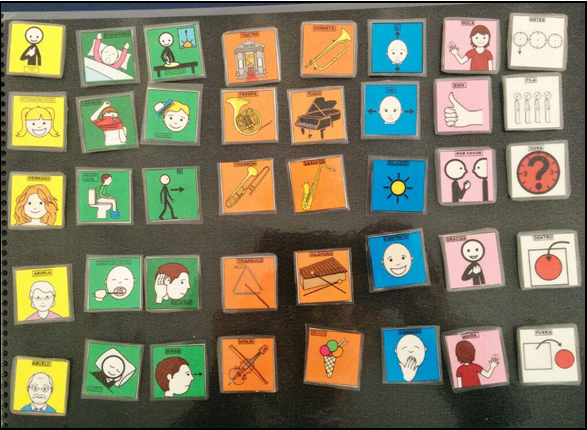
\includegraphics[width=0.7\linewidth]{Imagenes/Bitmap/tablerofisico}
	\caption{Pictographic board on which the user indicates what to communicate.}
	\label{fig:physicalboard}
\end{figure}


Communication boards are often created by teachers, parents or tutors to be used by a person with language difficulties. Traditionally they were made by cutting out and pasting pictograms on cardboard, but over time technological solutions have been implemented to facilitate this task. 

There are a multitude of applications that allow the creation of material based on pictograms, but they are generally limited to a specific format and offer little freedom to the user to create material. In addition, each of these applications has different options or facilities, such as translating a sentence into pictograms, a board where pictograms can be placed wherever you want, adding figures to the board, etc. But there is no single application that combines all these options. 
The purpose of this work is to create a web application that allows creating pictographic material quickly and easily, offering the greatest possible freedom to the user, and integrating the options most used and demanded by users in a single tool. 

\section{Objectives}
\label{cap1:sec:Objectives}



The aim of the work is to develop a web application that allows the creation of pictographic material by bringing together the functionalities most used and demanded by users. The application must have a board that allows to move with precision pictograms and other complementary elements.

For this purpose, the different existing applications will be investigated as well as the functionalities most demanded by users. Research will also be carried out into different web technologies.

Another objective is to create a simple and intuitive user interface that can be used in as many devices as possible. In order to verify the objectives of the work, an evaluation will be carried out to check the user-friendliness of the application. 


\section{Document structure}
\label{cap1:sec:mem}

The structure followed to organize this memory consists of the following chapters.
\begin{itemize}
	\item In chapter one, written in English and Spanish, it will set out the context in which the work has been carried out, also the motivation and objectives for doing so.
	
	\item Chapter two will explain briefly what a pictogram is and the different communication systems based on pictograms. In addition, the different tools related to pictograms will be discussed with an emphasis on editing communication boards.
	
	\item Chapter three will present the technologies used for the development of the application.
	
	\item Chapter four will specify the requirements and explain the created prototypes.
	
	\item Chapter five will detail the architecture and implementation of the application.
	
	\item Chapter six will show the design, results and analysis of the evaluation with users. 
	
	\item Chapter seven, written in English and Spanish, presents the final conclusions and specifies future work.
	
	\item Chapter eight will detail the tasks carried out by the two project participants.
\end{itemize}	





\end{otherlanguage}
\addtocounter{chapter}{-1} 
%%%%%%%%%%%%%%%%%%%%%%%%%%%%%%%%%%%%%%%%%%%%%%%%%%%%%%%%%%%%%%%%%%%%%%%%%%%

\chapter{Introducción}
\label{cap:introduccion}

\chapterquote{La inteligencia es la habilidad de adaptarse a los cambios}{Stephen Hawking}

\begin{resumen} En este capítulo se explicará la Motivación \ref{cap1:sec:Motivacion}, los objetivos que se quieren lograr inicialmente\ref{cap1:sec:Objetivos} y la estructura de esta memoria de TFG \ref{cap1:sec:Estructura}. 
\end{resumen}
\section{Motivación}
\label{cap1:sec:Motivacion}

Los humanos siempre hemos tenido la necesidad inherente de comunicarnos y quien no es capaz de hacerlo, generalmente acaba excluido. Y esa es la palabra clave, comunicación. Su origen proviene del latín, “\textit{communicare}”, difundir y este de “\textit{communis}” común. Gracias a ello, hemos podido llegar hasta donde estamos actualmente, una era donde todos pueden tener una voz. Por eso es más importante que nunca, no olvidarse de los que tienen dificultades. Para que puedan alzar su voz y difundir su palabra.

Sin embargo, en las últimas décadas ha habido un avance sin precedentes en el estudio e investigación sobre las discapacidades comunicativas. Éstos avances vinieron acompañados de herramientas y sistemas para facilitar la comunicación muchos de los cuales siguen vigentes a día de hoy. Uno de los principales perfiles que utilizan estos sistemas, son las  personas con trastorno del espectro autista (TEA)

Sin entrar en gran detalle, podemos encontrar que la gente con \textit{TEA} tienen dificultades en la comunicación verbal pues a menudo la comunicación no es recíproca o no se realiza en el contexto social adecuado. Respecto a la comunicación no verbal, también sufren dificultades al entender el significado de gestos faciales o expresión corporal de otras personas. Todo esto causa a menudo malentendidos, pues generalmente no se comprende el contexto y dificulta la comunicación. 

Para facilitar la comunicación se utilizan otros medios alternativos como los sistemas pictográficos, que permiten comunicarse mediante imágenes. Estos sitemas pictográficos, al estar compuestos por cientos de pictogramas habitualmente, están agrupados en \textbf{tableros pictográficos}. Estos tableros son superficies donde se colocan pictogramas para formar mensajes. Un ejemplo de tablero es el que vemos en la Figura \ref{fig:tablerofisico}. Hasta hace poco, dichos tableros eran creados a mano recortando y pegando los pictogramas pero con el tiempo se han desarrollado herramientas enfocadas a trabajar con tableros y pictogramas.

Para la elaboración de nuestra aplicación web tendremos en cuenta las aplicaciones de Pictar y PicTableros ya que ambos implementan herramientas que nos serán útiles de cara a la implementación. 

Durante este tiempo, además de estas herramientas, han surgido muchas más, cada una con sus características y funcionalidades únicas. Pero al final queda la sensación que nunca se podía hacer todo en un mismo lugar, y lo que le falta a una lo tiene otra herramienta, etc. Por ejemplo en las aplicaciones mencionadas previamente podemos ver que falta algún tipo de cuadrícula en el tablero para que a la hora de insertar los pictogramas estos queden perfectamente colocados y el tablero tenga una mejor apariencia visual.

En este contexto, la finalidad es crear una herramienta que unifique las mejores características de cada aplicación, además de permitir crear y editar tableros en un mismo lugar con la mayor facilidad posible. Afortunadamente, ya existe una base con la que nos podemos apoyar, gracias a proyectos de años anteriores como hemos mencionado, con ideas que se quedaron como trabajo futuro junto a las ideas propias. 


% TODO: \usepackage{graphicx} required
\begin{figure}[h!]
	\centering
	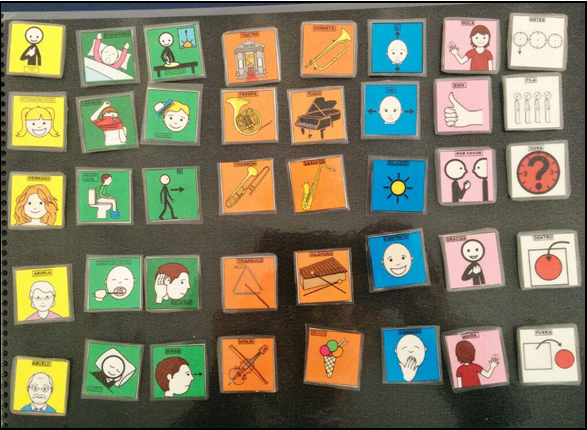
\includegraphics[width=0.7\linewidth]{Imagenes/Bitmap/tablerofisico}
	\caption{Tablero pictográfico en el que el usuario señala lo que quiere comunicar.}
	\label{fig:tablerofisico}
\end{figure}






\section{Objetivos}
\label{cap1:sec:Objetivos}

Teniendo en cuenta todos los temas que hemos tratado en la introducción queremos desarrollar una aplicación web multiplataforma que permite la edición de tableros y que incorpore una cuadrícula para ayudar a ajustar los pictogramas cuando se inserten. En la aplicación también se incorporarán herramientas de búsquedas de pictogramas por palabras y traducción de texto a pictograma.

Otro objetivo que nos hemos propuesto es que la aplicación pueda utilizarse en dos idiomas, por defecto la aplicación estará en español pero con una casilla para seleccionar el idioma se podrá cambiar a inglés. Este objetivo es sobre todo para ayudar y facilitar en el uso de esta aplicación a personas que no hablen español.

Para poder cumplir todos los objetivos mencionados se tendrá como referencia los TFG y TFM de Pictar y PicTableros. También se hará una labor de investigación en busca de nuevas tecnologías y herramientas con las que trabajar para desarrollar la aplicación. 

La forma en la que se comprobará el estado de los objetivos y su evolución será por medio de reuniones con los directores del TFG donde se analizará el trabajo realizado para ver el progreso, la forma en la que se van implementando los objetivos y la corrección de errores.



\section{Estructura de la memoria}
\label{cap1:sec:Estructura}

La estructura para memoria se encuentra dividida en [x] capítulos, a continuación se explicará brevemente su contenido. --según avancemos habrá que ir completándolo--
\begin{itemize}
	\item En los capítulos 1 y 2, se expondrá el contexto bajo el cual se ha realizado el trabajo junto a la motivación y objetivos para realizarlo.
	\item En el capítulo 3 se explicará qué es un pictograma y los distintos sistemas de comunicación con ellos. Además se analizarán las distintas herramientas relacionadas con pictogramas haciendo énfasis en la edición de tableros.
\end{itemize}	





\chapter{Estado de la Cuestión}
\label{cap:estadoDeLaCuestion}



\begin{resumen} En este capítulo se dará una idea general sobre los Sistemas aumentativos y alternativos de comunicación \ref{cap3:sec:saac}, las características de los pictogramas y los distintos sistemas pictográficos que existen \ref{cap3:sec:pictogramas}. Finalmente, se verán las distintos herramientas con las que se construyen tableros de pictogramas \ref{cap3:sec:editor-tableros}.

\end{resumen}


Los humanos siempre  han tenido la necesidad inherente de comunicarse y quien no es capaz de hacerlo generalmente acaba excluido. A día de hoy este problema sigue afectando a parte de la población como es el caso de las personas con Trastorno del Espectro Autista (\textit{TEA}).
\\

Sin entrar en gran detalle, podemos encontrar que la gente con \textit{TEA} tiene dificultades en la comunicación verbal, pues a menudo ésta no es recíproca o no se realiza en el contexto social adecuado. Respecto a la comunicación no verbal, también sufren dificultades al entender el significado de gestos faciales o expresión corporal de otras personas. Todo esto causa a menudo malentendidos, pues generalmente no se comprende el contexto y dificulta la comunicación. 


\section{Sistemas Aumentativos y Alternativos de Comunicación}
\label{cap3:sec:saac}
Los Sistemas Aumentativos y Alternativos de Comunicación (\textit{SAAC}) son las distintas formas de expresión sin tener en cuenta el lenguaje hablado que tiene como finalidad aumentar y/o compensar los problemas de comunicación de personas con discapacidad como por ejemplo trastornos del espectro autista, discapacidad intelectual, deficiencia auditiva, parálisis cerebral entre otros.

En ocasiones puede hacer falta el uso de recursos para poder comunicarse, es por ello que podemos distinguir dos tipos de \textit{SAAC}, los sistemas sin ayuda y los sistemas con ayuda.
\newpage
\begin{itemize}
	\item \textbf{Sistemas sin ayuda}: no utilizan ningún recurso externo para establecer la comunicación, únicamente usan su propio cuerpo. En los sistemas sin ayuda podemos observar dos tipos de grupos, los métodos gestuales (lengua de signos) y los métodos oralistas (lectura labiofacial). 
	\item \textbf{Sistemas con ayuda}: utilizan recursos externos para establecer la comunicación. Los más utilizados suelen ser pictogramas, imágenes o símbolos.
\end{itemize}

Las \textit{SAAC} utilizan múltiples recursos para poder comunicarse con personas con discapacidades cognitivas y entre todos ellos destacan los sistemas pictográficos. Se trata de uno de los sistemas más utilizados y esto es debido a su fácil comprensión ya que representan gráficamente lo que se desea transmitir como palabras o conceptos. 

\section{Pictogramas}
\label{cap3:sec:pictogramas}
Los pictogramas son imágenes o símbolos de rápida comprensión que expresan acciones, objetos, emociones, etc. Un conjunto de pictogramas en un cierto orden, pueden generar una oración. Todos ellos deben cumplir las siguientes características\footnote{\url{http://aularagon.catedu.es/materialesaularagon2013/arasaac/ZIPs/Modulo_1/contenidos.html}}:
\begin{enumerate}
	\item \textbf{Referencialidad}: relación del pictograma con el referente.
	\item \textbf{Ítems gráficos}: imágenes que representen de manera sencilla aquello que se toma como modelo.
	\item \textbf{Comprensión}: debe ser fácilmente entendible independientemente de la formación, idioma o discapacidad.
	\item \textbf{Legibilidad}: mantener una coherencia visual entre pictogramas.
	\item \textbf{Sencillez}: mostrar únicamente los elementos relevantes sin elementos distractores o adornos insignificantes.
\end{enumerate}


 
Existen numerosos sistemas pictográficos. A continuación hablaremos de algunos de los más relevantes:

\subsection{Sistema Pictográfico de Comunicación - SPC}

El Sistema Pictográfico de Comunicación\footnote{\url{https://www.uv.es/bellochc/logopedia/NRTLogo8.wiki?8}} (\textit{SPC}) fue creado en 1981 por Roxana Mayer Johnson, con la intención de facilitar la comunicación a quienes tienen un nivel de lenguaje expresivo simple o vocabulario limitado. Gracias a la diferenciación por colores, facilita la comprensión de la estructura sintáctica. Actualmente cuenta con más de 3000 iconos. Está organizado por seis colores según su función gramatical como podemos ver en la Figura \ref{fig:spccolores}.

\begin{itemize}
	\item \textbf{Personas} (Amarillo): representan a familiares y pronombres. Ejemplo: mamá, familia,  yo, ellos.
	\item \textbf{Verbos} (Verde): representan acciones. Ejemplo: abrir, agarrar, comer, ir.
	\item \textbf{Descriptivos} (Azul): representan descripciones, adjetivos y adverbios. Ejemplo: bonito, triste, vacío, lleno.
	\item \textbf{Nombre} (Naranja): representan objetos u otros elementos que no aparecen en otra categoría. Ejemplo: gato, almohada o casa.
	\item \textbf{Miscelánea} (Blanco): representa números, letras y colores
	\item \textbf{Social} (Rosa): vocabulario relacionado con relaciones sociales. Ejemplo: buenos días, sí, gracias, no lo sé.
	
\end{itemize}

% TODO: \usepackage{graphicx} required
\begin{figure}[h!]
	\centering
	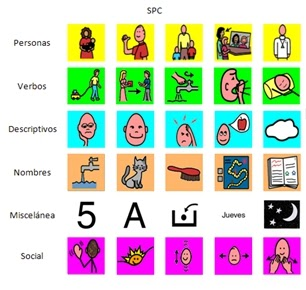
\includegraphics[width=0.7\linewidth]{Imagenes/Bitmap/SPCcolores}
	\caption{Ejemplo de categorías en SPC.}
	\label{fig:spccolores}
\end{figure}

\subsection{Blissymbolics}
Byssimbolics\footnote{\url{https://www.blissymbolics.org/index.php/about-blissymbolics}}
es un sistema de comunicación que fue usado por primera vez en 1971 para facilitar la comunicación con niños que padecían alguna discapacidad. Actualmente está compuesto por más de 5000 símbolos o  \textit{Bliss-Words} los cuales a su vez están compuestos por uno o más Caracteres-Bliss o  \textit{Bliss-Characters}. A pesar de que los 150 \textit{Bliss-Characters} que hay son sencillos de dibujar, requieren un periodo de aprendizaje para comprender su significado y así el de las \textit{Bliss-Words}. En la Figura \ref{fig:blisscharacters} vemos algunos \textit{Bliss-Characters} con su significado. \\
% TODO: \usepackage{graphicx} required

\begin{figure}[h!]
	\centering
	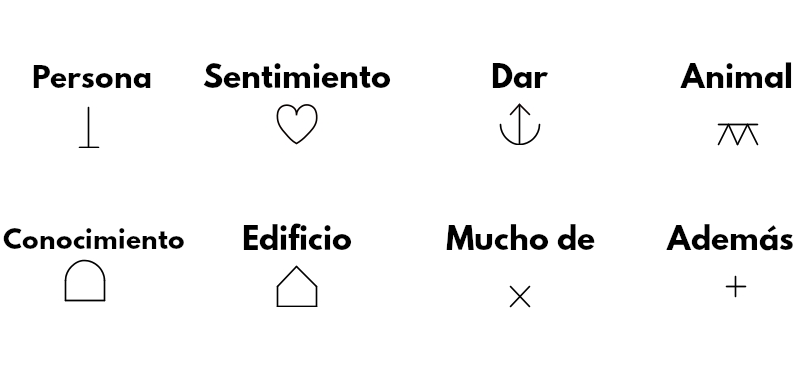
\includegraphics[width=0.8\linewidth]{Imagenes/Bitmap/BlissCharacters}
	\caption[Ejemplo de Bliss-Characters]{Ejemplo de Bliss-Characters.}
	\label{fig:blisscharacters}
\end{figure}
Una vez comprendido, en la Figura \ref{fig:blissword} vemos cómo se han combinado para generar \textit{Bliss-Words}. Destacar que el orden, el tamaño o la posición de los los Bliss-Characters, puede alterar su significado. Adicionalmente pueden estar agrupados de los mismos colores vistos en SPC.

% TODO: \usepackage{graphicx} required
\begin{figure}[h!]
	\centering
	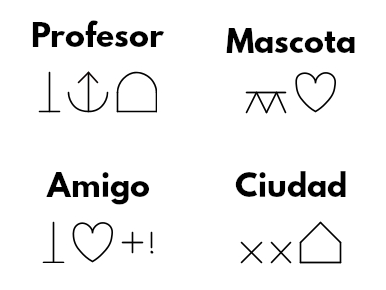
\includegraphics[width=0.4\linewidth]{Imagenes/Bitmap/BlissWord}
	\caption[Ejemplo de Bliss-Words]{Ejemplo de Bliss-Words.}
	\label{fig:blissword}
\end{figure}



\subsection{Sclera}
La principal característica de Sclera\footnote{\url{https://www.sclera.be/en/picto/overview}} frente a otros sistemas pictográficos es que sus pictogramas son menos coloridos pero cuentan con pictogramas más avanzados en cuanto a acciones representadas. Un ejemplo de ello se puede ver en la Figura \ref{fig:sclera} donde la acción de pedir atención se puede realizar de dos maneras posibles. Cuenta con un total de 11.497 pictogramas en español.

En la actualidad el desarrollo de Sclera está paralizado desde 2015.



% TODO: \usepackage{graphicx} required
\begin{figure}[h!]
	\centering
	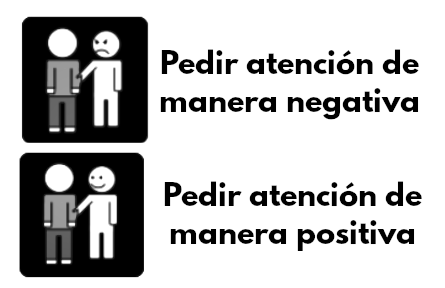
\includegraphics[scale=0.5]{Imagenes/Bitmap/Sclera}
	\caption{Ejemplo de acciones en Sclera.}
	\label{fig:sclera}
\end{figure}

\newpage
\subsection{Mulberry Symbols}
Mulbery Symbols\footnote{\url{https://mulberrysymbols.org/}} se creó con el propósito de ser un sistema pictográfico orientado a adultos ya que un gran porcentaje de dichos sistemas estaban pensados principalmente para niños y dificultaban la comunicación por falta de pictogramas. Como se observa en la Figura \ref{fig:mulberry} podemos ver ejemplos de pictogramas enfocados a adultos como cerveza o fumar.

Todos los pictogramas se pueden descargar gratuitamente desde su página web en formato ZIP cuyas imágenes se encuentran en formato SVG o en formato CSV donde están categorizados según su nombre y categoría. 
Los pictogramas de Mulbery cuentan con 118 categorías incluyendo sustantivos, pronombres, verbos sumando un total de 3.436 pictogramas. A diferencia de otros sistemas pictográficos Mulbery sigue en activo añadiendo constantemente nuevos pictogramas. 

Los pictogramas de Mulbery son utilizados por muchas aplicaciones como BoradBuilder\footnote{\url{ https://globalsymbols.com/boardbuilder/boardsets}} (aplicación web para diseñar tableros de comunicación), Cboard\footnote{\url{https://www.cboard.io/}} (aplicación web de comunicación que usa pictogramas y conversión de texto a voz) o CommuniKate\footnote{\url{http://communikate.equalitytime.co.uk/}} (página web que ofrece tableros diseñados en Powerpoint o Impress). Una de las últimas herramientas creadas que hace uso de los pictogramas de Mulbery es la diseñada por Eliada Pampoulou y Maria Constanta de la Universidad Tecnológica de Chipre la cual usa unas plantillas imprimibles en inglés\footnote{\url{https://mulberrysymbols.org/assets/COVID19/Covid-19_AAC-EN.pdf}} o griego para ayudar a la comunicación de los pacientes con la COVID-19 que tienen dificultades para comunicarse.



% TODO: \usepackage{graphicx} required
\begin{figure}[h!]
	\centering
	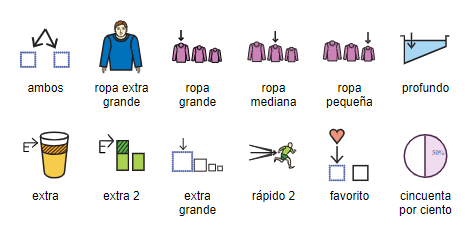
\includegraphics[scale=0.2]{Imagenes/Bitmap/Mulberry}
	\caption{Ejemplo de pictogramas de Mulberry.}
	\label{fig:mulberry}
\end{figure}

\newpage
\subsection{Minspeak}
Minspeak\footnote{\url{http://ares.cnice.mec.es/informes/18/contenidos/94.htm}}. es un sistema de comunicación alternativo creado por Bruce Baker en 1982. Difiere con los vistos anteriormente en que el significado de los iconos no viene preestablecido sino que es acordado entre usuario y logopeda. Es por ello que cada icono acordado tenga un significado distinto según la secuenciación de iconos. Por ejemplo en el caso de la Figura \ref{fig:minspeak} la asociación del icono casa junto a la cama, en ese orden podría ser interpretado como dormitorio. 

% TODO: \usepackage{graphicx} required
\begin{figure}[h!]
	\centering
	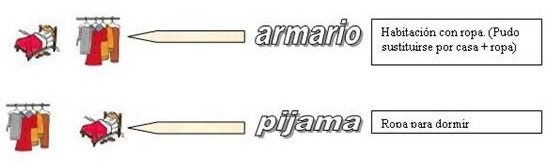
\includegraphics[width=0.7\linewidth]{Imagenes/Bitmap/Minspeak}
	\caption{Ejemplo de Minspeak.}
	\label{fig:minspeak}
\end{figure}

Como cada pictograma puede tener un significado distinto según su orden, se crearon Programas de Comunicación Minspeak (\textit{PAM}). Éstos se usan para cuando una casilla o icono haya sido seleccionada, se activen los posibles iconos con los que pueda tener algún tipo de relación. Inicialmente se creó hardware específico como aparece en la Figura \ref{fig:chatbox} con 16 celdas las cuales podía generar hasta 1024 mensajes, los teclados evolucionaron con más celdas y combinaciones, hasta pasar a teclados digitales implementados por software como PortaVoz\footnote{\url{http://www.terapia-ocupacional.com/articulos/Portavoz_JMLedesma.shtml}}.

% TODO: \usepackage{graphicx} required
\begin{figure}[h!]
	\centering
	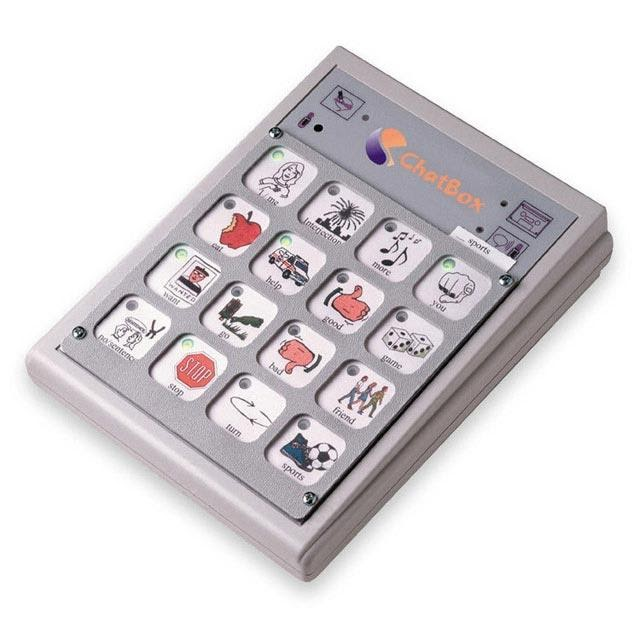
\includegraphics[width=0.4\linewidth]{Imagenes/Bitmap/ChatBox}
	\caption[ChatBox]{Panel de ChatBox}
	\label{fig:chatbox}
\end{figure}



\subsection{ARASAAC}

El portal Aragonés de Comunicación Aumentativa y Alternativa \\ \textit{ARASAAC}\footnote{\url{http://www.arasaac.org/}}
 surge en 2007 gracias a la colaboración entre el personal del CATEDU, el colegio público de educación Especial Alborada y del Centro Politécnico Superior de la Universidad de Zaragoza. Su objetivo era la creación de un sistema pictográfico de libre distribución que ayudara en el ámbito de la comunicación a todas aquellas personas que lo necesitasen.
Actualmente el portal de \textit{ARASAAC} incluye fotografias, videos y cuenta con más de 39000 pictogramas tanto a color como en blanco y negro y con traducciones a 20 idiomas. También ofrece herramientas online con las que poder generar materiales como por ejemplo generador de calendarios, generador de tableros, creador de símbolos, etc.

A diferencia de otros sistemas pictográficos, \textit{ARASAAC} permite una gran cantidad de opciones configurables como el color de fondo, marco o tiempo verbal, la Figura \ref{fig:configuarcion-arasaac} muestra todas las posibles opciones de configuración.



\begin{figure}[h!]
	\centering
	\includegraphics[width=0.7\linewidth]{Imagenes/Bitmap/Configuarción ARASAAC}
	\caption{Opciones de configuración de un pictograma.}
	\label{fig:configuarcion-arasaac}
\end{figure}



En la actualidad \textit{ARASAAC} es uno de los sistemas pictográficos más utilizados a nivel de educación especial en España. Sus pictogramas se utilizan en colegios, universidades e incluso se han creado asociaciones para facilitar su implantación. CreaTea es una asociación en la Comunidad de Madrid cuyo objetivo es habilitar lugares como clínicas, restaurantes o ayuntamientos, para ayudar a la inclusión de personas con dificultades en la comunicación y concienciar a la sociedad.

También cabe destacar que \textit{ARASAAC} ha recibido varios premios por su labor y que es una herramienta utilizada en varios países por lo que la cantidad de usuarios que colaboran es muy alta. Esto queda reflejado en la cantidad de pictogramas que se publican a la plataforma por parte de colaboradores sin ánimo de lucro y dichos pictogramas están constantemente actualizándose. Un ejemplo de ellos son los pictogramas que se han publicado debido a la pandemia como por ejemplo las Figuras \ref{fig:picto-mascarilla} y \ref{fig:picto-mascarilla-mal-colocada}.

\newpage
% TODO: \usepackage{graphicx} required
\begin{figure}[h!]
	\centering
	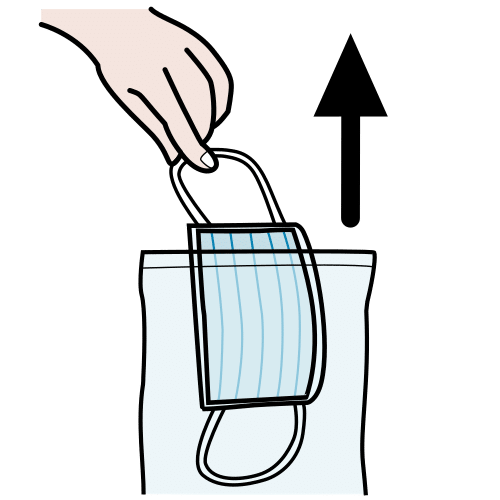
\includegraphics[width=0.2\linewidth]{Imagenes/Bitmap/Picto Mascarilla}
	\caption{Acción de sacar la mascarilla.}
	\label{fig:picto-mascarilla}
\end{figure}

\begin{figure}[h!]
	\centering
	
\includegraphics[width=0.2\linewidth]{Imagenes/Bitmap/Mascarilla mal colocada}
	\caption{Pictograma que representa mascarilla mal colocada.}
	\label{fig:picto-mascarilla-mal-colocada}
\end{figure}

En la Figura \ref{fig:arasaacpictos} podemos ver algunos ejemplos de pictogramas de \textbf{ARASAAC} en situaciones o casos más cotidianos. Destacan la manera clara y concisa en la que están representados. 

% TODO: \usepackage{graphicx} required
\begin{figure}[h!]
	\centering
	
\includegraphics[width=0.7\linewidth]{Imagenes/Bitmap/ARASAACPictos}
	\caption{Ejemplo de pictogramas más típicos de \textit{ARASAAC}.}
	\label{fig:arasaacpictos}
\end{figure}

La licencia de \textit{ARASAAC} es de tipo \textit{Creative Commons (BY-NC-SA)} por lo que se podrá utilizar el material elaborado por ellos de cara a la implementación del Trabajo Fin de Grado. Utilizaremos sus pictogramas publicados en su página web y la API que han desarrollado para acceder a pictogramas de su base de datos.

\section{Editores de Tableros basados en Pictogramas}
\label{cap3:sec:editor-tableros}

Ya hemos visto multitud de sistemas pictográficos, pero para trabajar con ellos es necesario que sean fáciles de acceder, pues es fácil encontrar cientos de pictogramas en cada sistema pictográfico. La solución a esto, son los tableros pictográficos. Los tableros son un área en la que se pueden colocar pictogramas, fotografías o palabras que la persona indicará para comunicarse. Pueden tener distintas funciones, como por ejemplo hacer un horario, normas, o elegir entre distintas opciones mediante pictogramas. A menudo estos tableros se realizan mediante piezas de papel recortadas, como podemos ver en la Figura \ref{fig:editorespictogramas}.

% TODO: \usepackage{graphicx} required
\begin{figure}[h!]
	\centering
	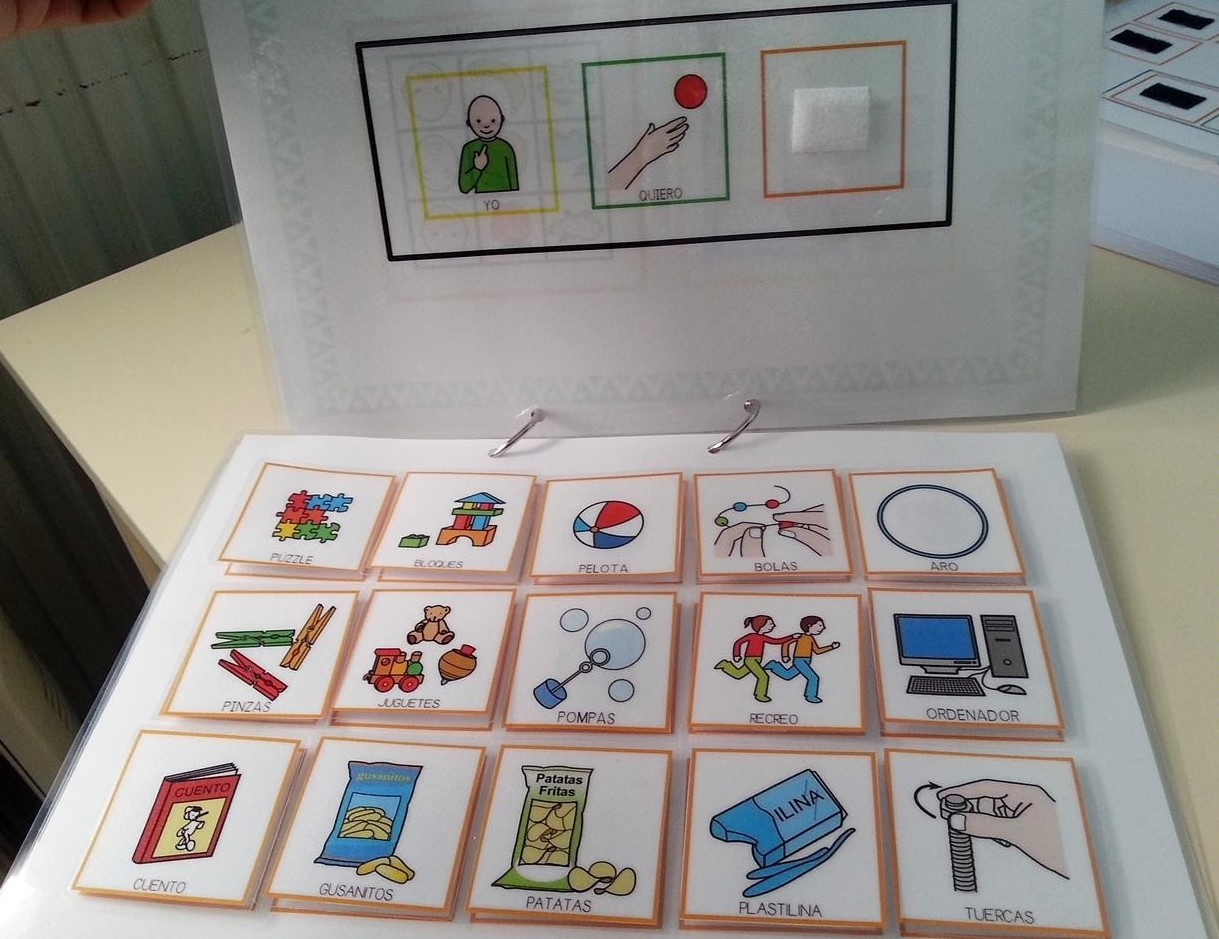
\includegraphics[width=0.7\linewidth]{Imagenes/Bitmap/EditoresPictogramas}
	\caption{Ejemplo de tablero para pictogramas en papel.}
	\label{fig:editorespictogramas}
\end{figure}

Estos tableros\footnote{\url{http://burbujadelenguaje.blogspot.com/2016/05/tablero-de-comunicacion-tea.html}}, no tienen por qué limitarse a un espacio rectangular, sino que se pueden usar de maneras más creativas dependiendo de las discapacidades de la persona que lo use. Por ejemplo los \textit{ETRAN}\footnote{\url{http://psicosociosanitario.blogspot.com/2016/05/tableros-de-comunicacion.html}}. (“Eye-Transfer”) son usados por gente con baja movilidad y que apuntan al pictograma con la mirada, otra persona está al otro lado del \textit{ETRAN} para ver qué pictograma está mirando como podemos ver en la Figura \ref{fig:tablero}. Otro ejemplo son los cuadernos de comunicación que como su nombre indica son un conjunto de hojas o tableros con símbolos básicos.

% TODO: \usepackage{graphicx} required
\begin{figure}[h!]
	\centering
	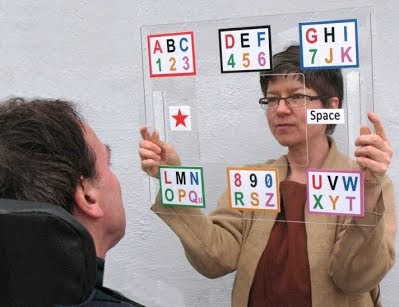
\includegraphics[width=0.7\linewidth]{Imagenes/Bitmap/Tablero}
	\caption{Uso de tablero ETRAN.}
	\label{fig:tablero}
\end{figure}

Trabajar con piezas de papel puede resultar engorroso y a menudo poco eficiente, por eso ha sufrido una evolución natural al medio digital, y con ello software de edición de tableros pictográficos. Gracias a ello, podremos ahorrar mucho trabajo, como buscar pictogramas, alinearlos, editarlos o incluso poder compartir los tableros.


Para crear y editar tableros se han creado multitud de aplicaciones, a continuación estudiaremos sus características.



\subsection{Pictoselector}
Es una herramienta gratuita para crear agendas visuales. Recopila más de 28.000 provenientes de \textbf{\textit{Sclera}}, \textbf{\textit{Mulberry}}, \textbf{\textit{ARASAAC}}, etc. Al crear un proyecto, permite cargar una plantilla o crear una desde cero. Se puede modificar el número de filas y columnas, la posición del texto y el tamaño del borde de los pictogramas.
\footnote{\url{ https://www.pictoselector.eu/es/ }}

% TODO: \usepackage{graphicx} required
\begin{figure}[h!]
	\centering
	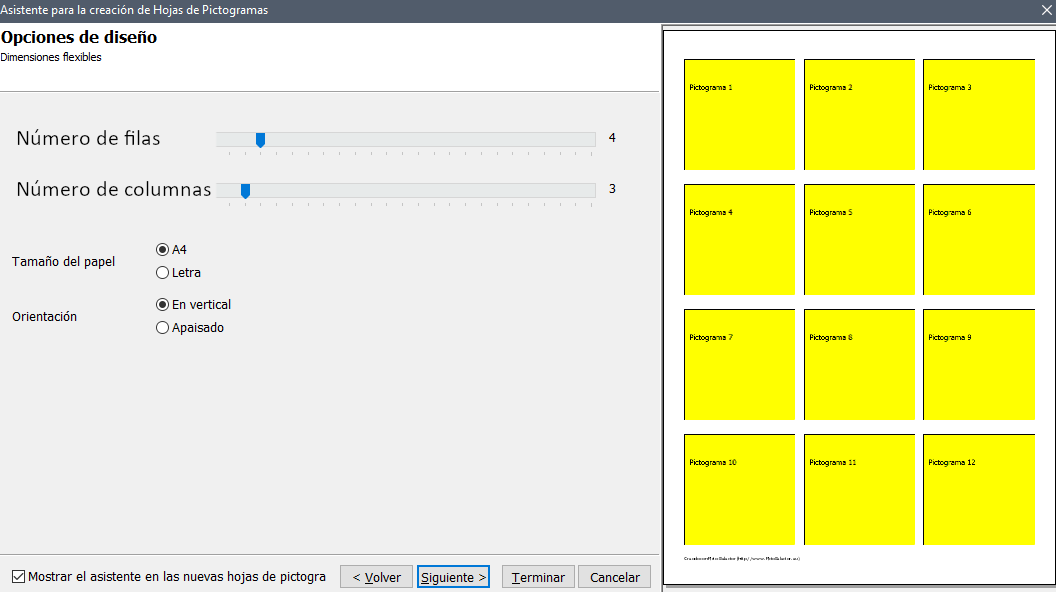
\includegraphics[width=0.7\linewidth]{Imagenes/Bitmap/Pictoselector Tablero}
	\caption{Ventana donde se edita el tamaño de la cuadrícula.}
	\label{fig:pictoselector-tablero}
\end{figure}


Una vez creado el tablero, podemos insertar en su cuadrícula distintos elementos, muchos de ellos en forma de pictograma. Para facilitar esta tarea, la cabecera de la aplicación contiene acceso directo a la inserción de pictogramas



Como podemos ver, de izquierda a derecha, existe un buscador de pictogramas que incluye la función de filtrar por juego de pictogramas. Además de poder editar ligeramente el picto ya sea coloreándolo o añadiendo un signo de pasado, presente o plural. Para el marcaje de tiempo pueden incluirse con facilidad pictogramas de reloj que marcan la hora y de duración que marcan un intervalo de tiempo. Adicionalmente se puede importar imágenes propias, códigos QR , texto o emoticonos.

% TODO: \usepackage{graphicx} required
\begin{figure}[h!]
	\centering
	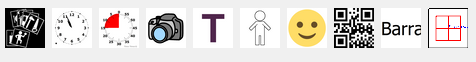
\includegraphics[width=0.7\linewidth]{Imagenes/Bitmap/Ribbon Pictoselector}
	\caption{Barra de inserción de pictogramas.}
	\label{fig:ribbon-pictoselector}
\end{figure}

% TODO: \usepackage{graphicx} required
\begin{figure}[h!]
	\centering
	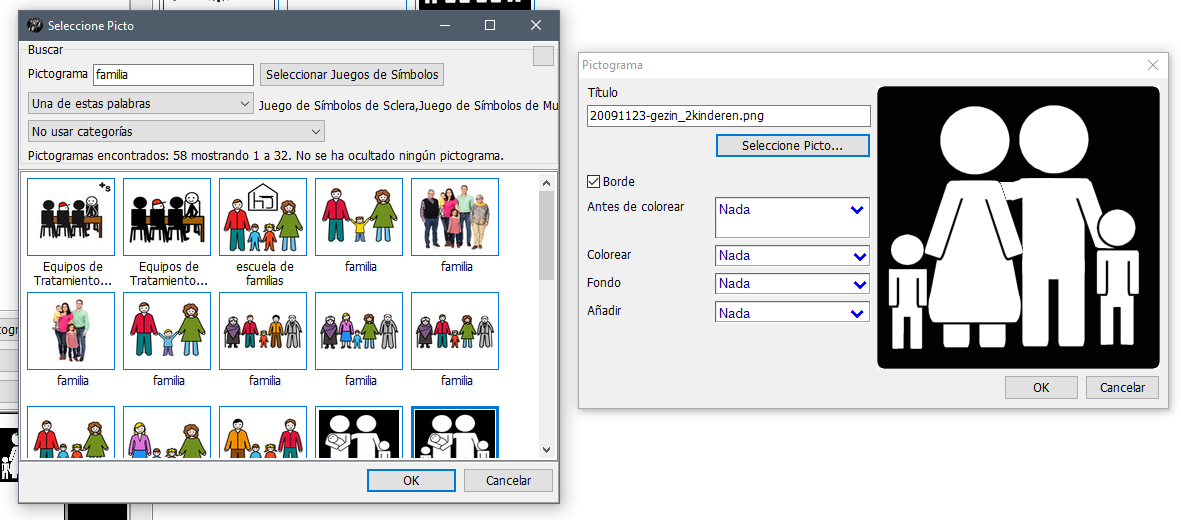
\includegraphics[width=0.7\linewidth]{Imagenes/Bitmap/Editor y buscador de pictoselector}
	\caption{Buscador y editor de Pictogramas.}
	\label{fig:editor-y-buscador-de-pictoselector}
\end{figure}




El mayor inconveniente de la aplicación, pese a ser muy completa respecto a la búsqueda y edición de pictos, es su limitación de colocación a una cuadrícula.

\subsection{Editor ARASAAC}
La página web de \textit cuenta con herramientas online las cuales podemos usar para generar materiales .
\begin{itemize}
\item \textbf{Creador de animaciones}: genera una animación con los pictogramas que queramos en formato GIF o SWF. También permite configurar el intervalo entre los pictogramas y el número de repeticiones que hará.

\item \textbf{Creador de símbolos}: permite la personalización de pictogramas donde podremos cambiar el nombre del pictograma, poner su traducción, modificar la fuente del texto, poner un marco, ampliar la imagen y cambiar el fondo.

\item \textbf{Generador de frases}: consta de un total de tres pasos a seguir, el primero de ellos consiste en seleccionar las palabras que queramos traducir a pictogramas, el segundo paso nos mostrará todos los pictogramas asociados para cada palabra introducida y deberemos seleccionar el que más nos guste y el tercer paso aparecerán todos los pictogramas colocados en una tabla la cual podremos modificar.
\footnote{\url{ http://www.arasaac.org/herramientas.php }}

% TODO: \usepackage{graphicx} required
\begin{figure}[h!]
	\centering
	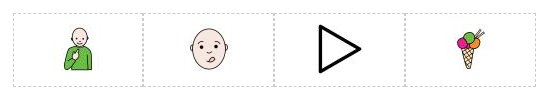
\includegraphics[width=0.7\linewidth]{Imagenes/Bitmap/Frase ARASAAC}
	\caption{Ejemplo con generador de frases.}
	\label{fig:frase-arasaac}
\end{figure}


\item \textbf{Generador de horarios}: genera un horario donde previamente tendremos que configurar una plantilla con los días, horas, el formato (horizontal o vertical), idioma, bordes del horario, texto para cada día y hora y la opción de insertar un pictograma en función de su día y hora.

\item \textbf{Generador de calendarios}: genera un calendario donde tendremos que especificar el mes, año e idioma deseado. Al igual que en el generador de horarios permite la opción de modificar el texto, colores, bordes y la posibilidad de poner un pictograma para cada día del mes.

\item \textbf{Generador de tableros}: crea un tablero con el número de filas y columnas deseado donde para cada casilla podremos insertar un pictograma. Al igual que en otras herramientas permite la modificación de colores, bordes y  texto del tablero.

\item \textbf{Creador de juegos}: genera una plantilla en formato .rtf para poder jugar al bingo, oca, dominós y dominós encadenados con los pictogramas que deseemos.
\end{itemize}

% TODO: \usepackage{graphicx} required
\begin{figure}[h!]
	\centering
	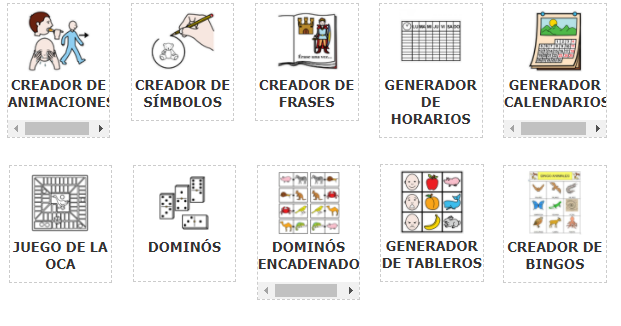
\includegraphics[width=0.4\linewidth]{Imagenes/Bitmap/Tableros ARASAAC}
	\caption[Tableros web ARASAAC]{Herramientas online que ofrece ARASAAC.}
	\label{fig:tableros-arasaac}
\end{figure}

\newpage
\subsection{Piktoplus}
Se trata de una aplicación para dispositivos Android. Su particularidad es que permite la creación de un avatar tridimensional personalizable\footnote{\url{http://www.aulautista.com/2013/12/05/piktoplus-un-comunicador-android-muy-especial/ }}. Dicho avatar será usado en los tableros pictográficos pues será quien protagonice las acciones. Permite registrar múltiples usuarios, cada uno con su propio avatar. Otra particularidad de Piktoplus son los sub-tableros. \footnote{\url{https://fatimamikel.wordpress.com/2014/04/17/piktoplus-2/ }}  Por ejemplo, en la Figura \ref{fig:piktoplus1}  hay un tablero con dos pictogramas, “Estoy” y “Me duele”.


% TODO: \usepackage{graphicx} required
\begin{figure}[h!]
	\centering
	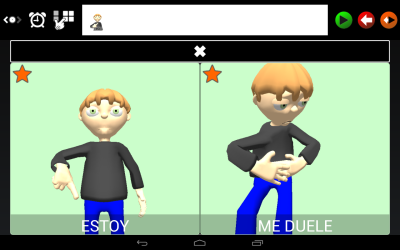
\includegraphics[width=0.5\linewidth]{Imagenes/Bitmap/Piktoplus1}
	\caption[Pictoplus tablero]{Ejemplo de tablero en Piktoplus}
	\label{fig:piktoplus1}
\end{figure}

En el caso que pusemos sobre estoy, se desplegará un sub-tablero dentro del mismo tablero con cuatro pictogramas como se representa en la Figura \ref{fig:piktoplus2}.


% TODO: \usepackage{graphicx} required
\begin{figure}[h!]
	\centering
	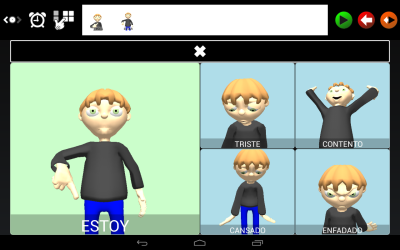
\includegraphics[width=0.5\linewidth]{Imagenes/Bitmap/Piktoplus2}
	\caption[Subtablero Piktoplus]{Subtablero en Piktoplus}
	\label{fig:piktoplus2}
\end{figure}


Respecto a la creación y edición de tableros, se trata de una cuadrícula sobre la cual se colocan los pictogramas, además permite aumentar el tamaño de los pictos. Por ejemplo “Estoy” ocupa cuatro celdas más que “Contento”. 

Actualmente esta aplicación no está disponible para descargar en tiendas de aplicaciones  habituales y su desarrollo ha cesado desde 2018. Aunque no esté disponible, plantea una idea muy interesante como la posibilidad de desplegar un sub-tablero a partir de un pictograma para mostrar pictogramas relacionados entre ellos.

\subsection{BoardMaker}
VER A FINALES DE MES PARA UNA POSIBLE ACTUALIZACIÓN DE APP

\subsection{Pictar}
Pictar\footnote{\url{ http://hypatia.fdi.ucm.es/pictar/}} es una aplicación web desarrollada por el alumno Alejandro Martín Guerrero de la Universidad Complutense de Madrid del grado de ingeniería informática como Trabajo de Fin de Máster. El propósito de Pictar es poder tener una aplicación web accesible desde cualquier dispositivo con conexión a internet para facilitar la comunicación a personas con TEA.

Pictar ofrece tres herramientas en su página web:
\begin{itemize}
	\item \textbf{Traducir frase}:permite generar una secuencia de pictogramas asociados a una frase o texto introducido por el usuario. Ofrece la posibilidad tras haber generado la secuencia de pictogramas, de poder cambiarlos por otros pictogramas del mismo significado mediante unas flechas que se encuentran tanto encima como debajo de cada pictograma. También incluye un icono que tiene como finalidad copiar la secuencia de pictogramas generados al tablero, ver la Figura \ref{fig:traducirfrase}.
	
	% TODO: \usepackage{graphicx} required
	\begin{figure}[h!]
		\centering
		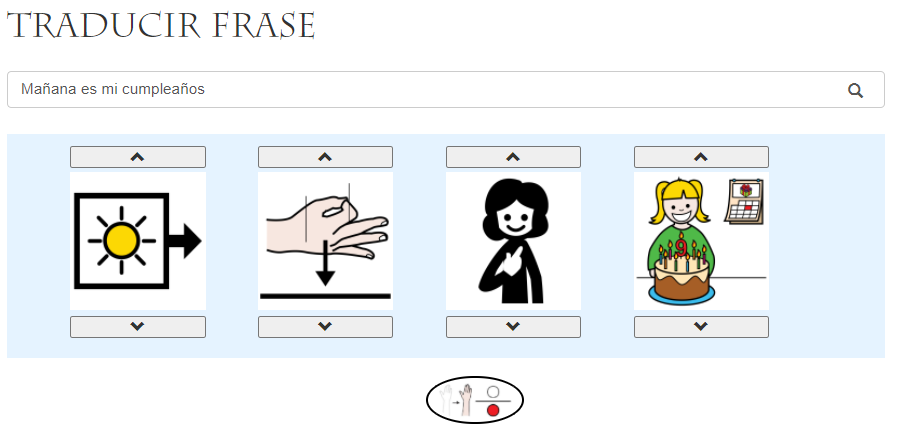
\includegraphics[width=0.7\linewidth]{Imagenes/Bitmap/TraducirFrase}
		\caption{Funcionalidad en la aplicación Pictar de traducir frase.}
		\label{fig:traducirfrase}
	\end{figure}

	\item \textbf{Buscador}: al introducir una palabra en el campo de búsqueda nos mostrará todos aquellos pictogramas con un significado igual o similar a la palabra introducida, ejemplo de ello en la Figura \ref{fig:buscador}. El buscador ofrece la posibilidad de poder arrastrar los pictogramas para insertarlos al tablero que se muestra en la Figura \ref{fig:editor}.
	
	% TODO: \usepackage{graphicx} required
	\begin{figure}[h!]
		\centering
		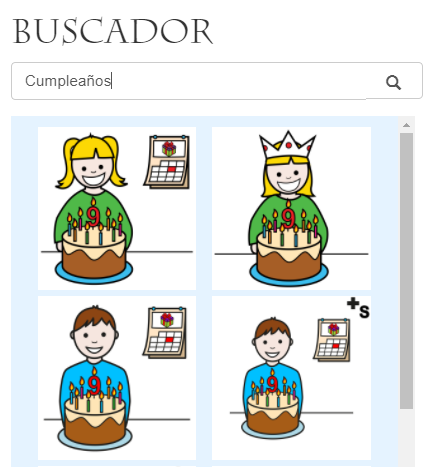
\includegraphics[width=0.5\linewidth]{Imagenes/Bitmap/buscador}
		\caption{Funcionalidad en la aplicación Pictar de buscador.}
		\label{fig:buscador}
	\end{figure}
	
	
	\item \textbf{Editor}: permite generar un tablero de pictogramas en el que deberemos seleccionar cuantos elementos va a tener en total y el número de columnas en los que se divide. Para añadir pictogramas al tablero tenemos dos opciones: la primera de ella es copiar la secuencia generada al traducir una frase a pictogramas y la segunda buscar un pictograma en el buscador para poder arrastrar el pictograma deseado al tablero. Por cada pictograma insertado en el tablero tendremos dos opciones debajo de éste situadas en las esquinas inferiores izquierda y derecha que permiten eliminar o dejar la casilla en blanco. El editor ofrece la posibilidad de añadir el nombre a cada pictograma, poner todos los pictogramas a color o blanco y negro y exportar o importar el tablero. Todas estas características se pueden observar en la Figura \ref{fig:editor}.
	
	% TODO: \usepackage{graphicx} required
	\begin{figure}[h!]
		\centering
		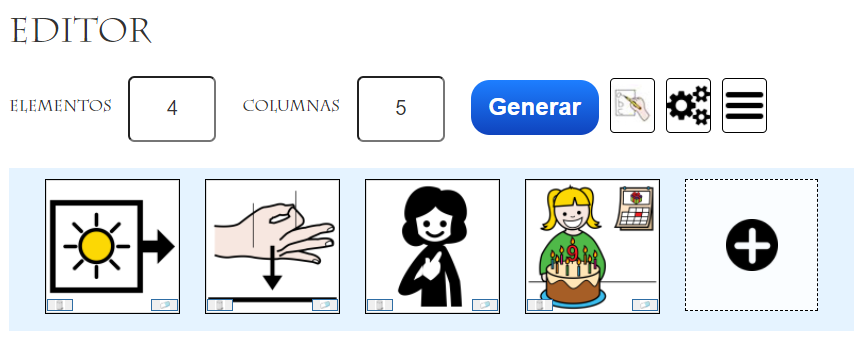
\includegraphics[width=0.7\linewidth]{Imagenes/Bitmap/editor}
		\caption{Funcionalidad en la aplicación Pictar de editor.}
		\label{fig:editor}
	\end{figure}
	
	
\end{itemize}




\newpage
\subsection{Pictableros}
\footnote{\url{ https://holstein.fdi.ucm.es/picto-tableros/  }}
Pictableros es una aplicación web de edición y creación de tableros y plantillas para pictogramas. Tiene dos partes diferenciadas:

\begin{itemize}
	\item Las plantillas sirven para que otros usuarios que quieran crear un tablero similar puedan sustituir con facilidad los pictogramas. Por ejemplo en la Figura \ref{fig:pictableros1} existe una plantilla de tablero para elegir un deporte, dicha plantilla puede ser modificada para sustituir el pictograma de balonmano por tenis. Estas plantillas pueden ser públicas o privadas.
	
	\item Los tableros públicos no pueden ser modificados, aunque  se puede crear una copia de ellos y modificarse para superponer símbolos (Bien, mal, amarillo, azul)
	

\end{itemize}

	% TODO: \usepackage{graphicx} required
	\begin{figure}[h!]
		\centering
		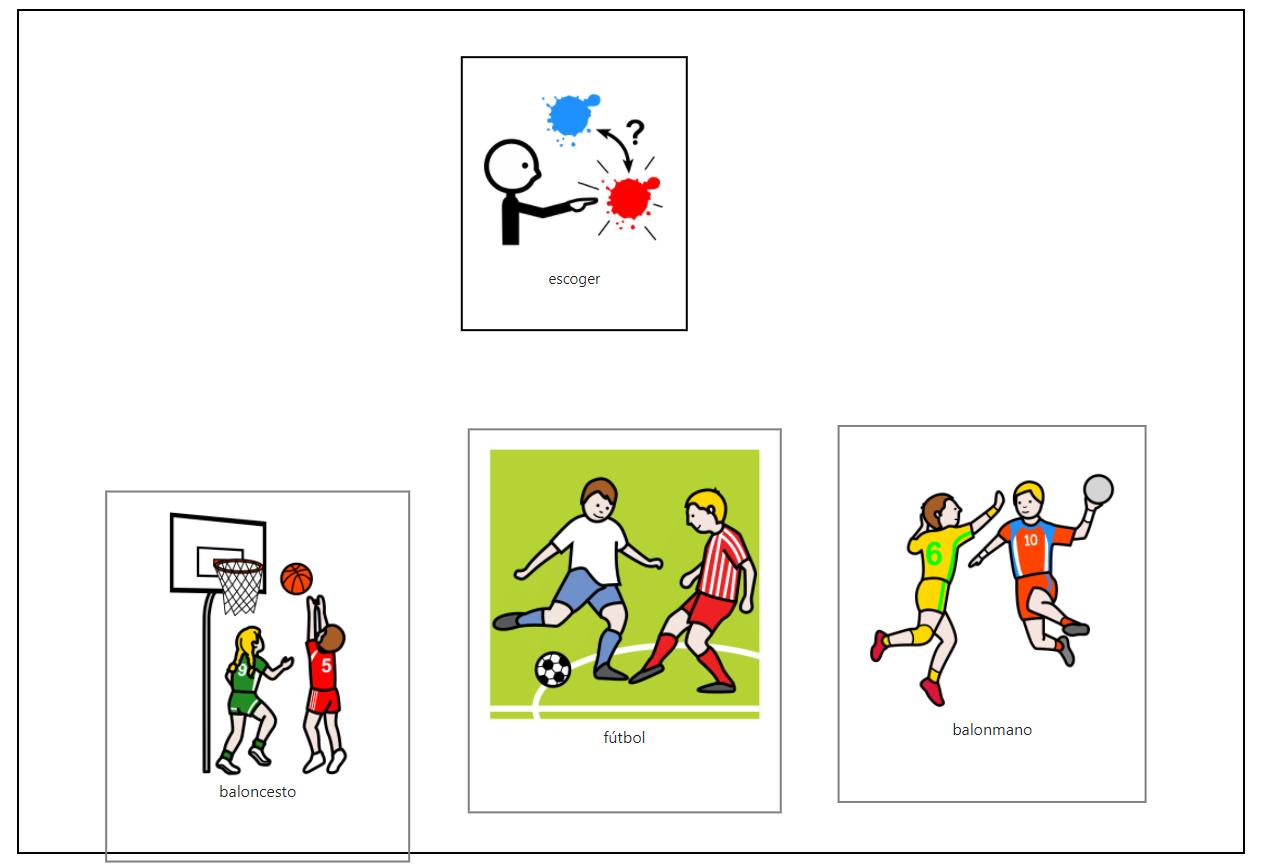
\includegraphics[width=0.7\linewidth]{Imagenes/Bitmap/pictableros1}
		\caption{Plantilla de elección de deporte.}
		\label{fig:pictableros1}
	\end{figure}
	
	
	% TODO: \usepackage{graphicx} required
	\begin{figure}[h!]
		\centering
		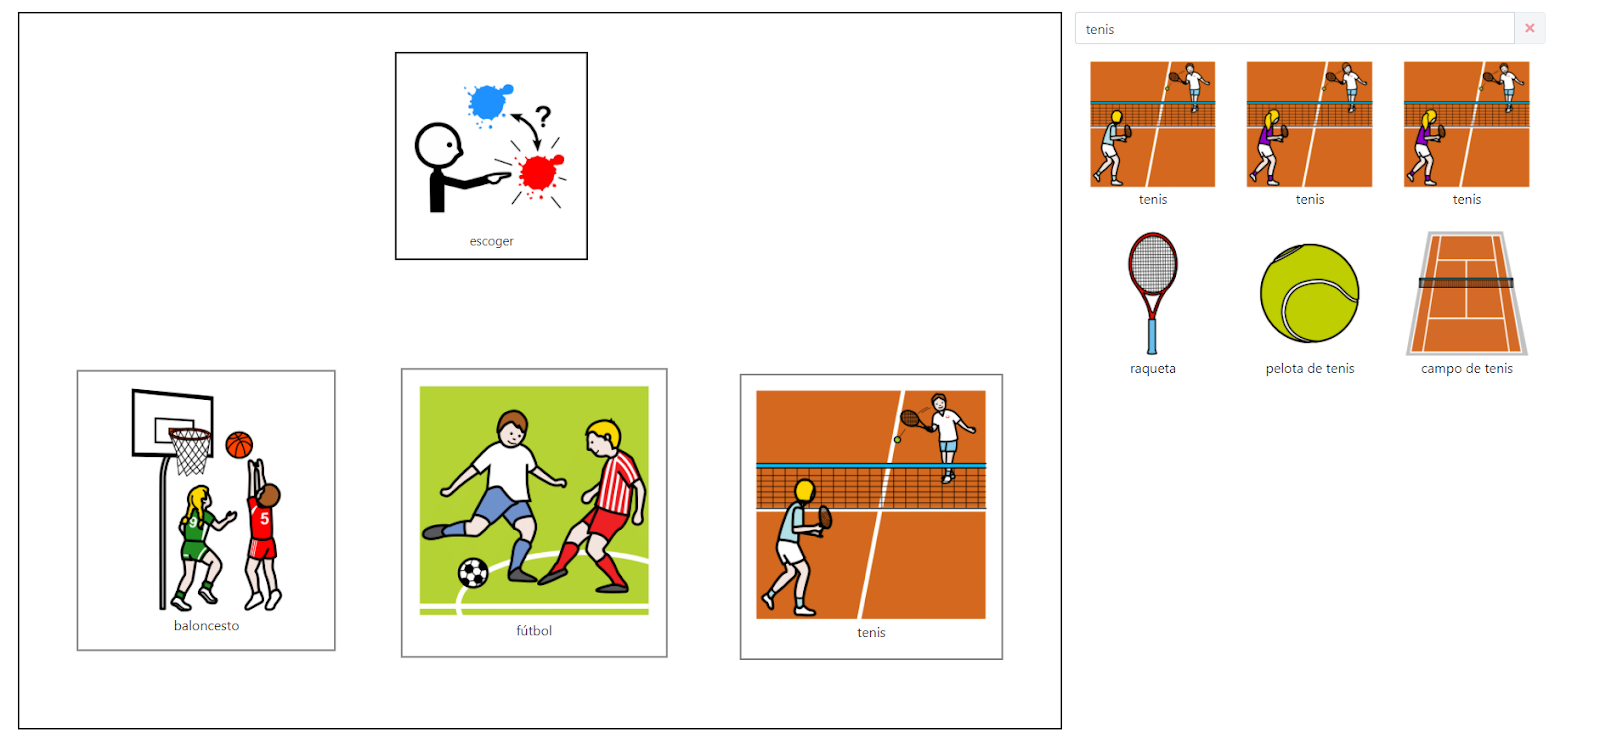
\includegraphics[width=0.7\linewidth]{Imagenes/Bitmap/pictableros2}
		\caption[Edición de plantilla en Pictableros]{Edición de plantilla de selección de deporte, sustituimos balonmano por tenis, haciendo uso del buscador de pictogrmas.}
		\label{fig:pictableros2}
	\end{figure}
	
	% TODO: \usepackage{graphicx} required
	\begin{figure}[h!]
		\centering
		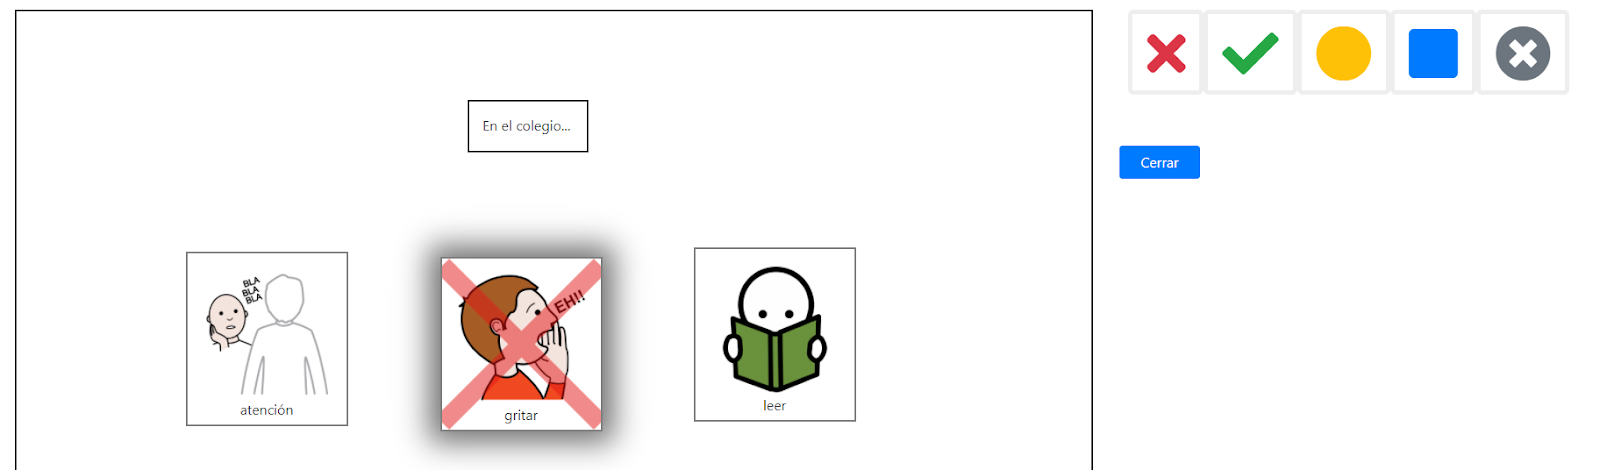
\includegraphics[width=0.7\linewidth]{Imagenes/Bitmap/pictableros3}
		\caption[Edición plantilla en Pictableros]{Edición de tableros, permite superponer un signo al pictograma.}
		\label{fig:pictableros3}
	\end{figure}
	

	


\newpage	
\subsection{Symbo Talk}

SymboTalk permite la creación de tableros de comunicación aumentativa y locución de tableros y pictogramas mediante su aplicación web o dispositivos móviles como Android e iOS.
\footnote{\url{  https://civat.es/app/symbo-talk/ }}
\footnote{\url{   http://aulaabierta.arasaac.org/symbotalk-0-inicio-2  }}
SymboTalk ofrece dos modos de usuario:

\begin{itemize}
	\item \textbf{Modo edición}: permite la creación de pictogramas, construir tableros, buscar pictogramas en un buscador. También ofrece la opción de crear un perfil y poder guardar todos los tableros que hayamos realizado.
	
	\item \textbf{Modo usuario}: pensado para que el usuario pueda comunicarse de una forma más fácil e intuitiva.
	
\end{itemize}

% TODO: \usepackage{graphicx} required
\begin{figure}[h!]
	\centering
	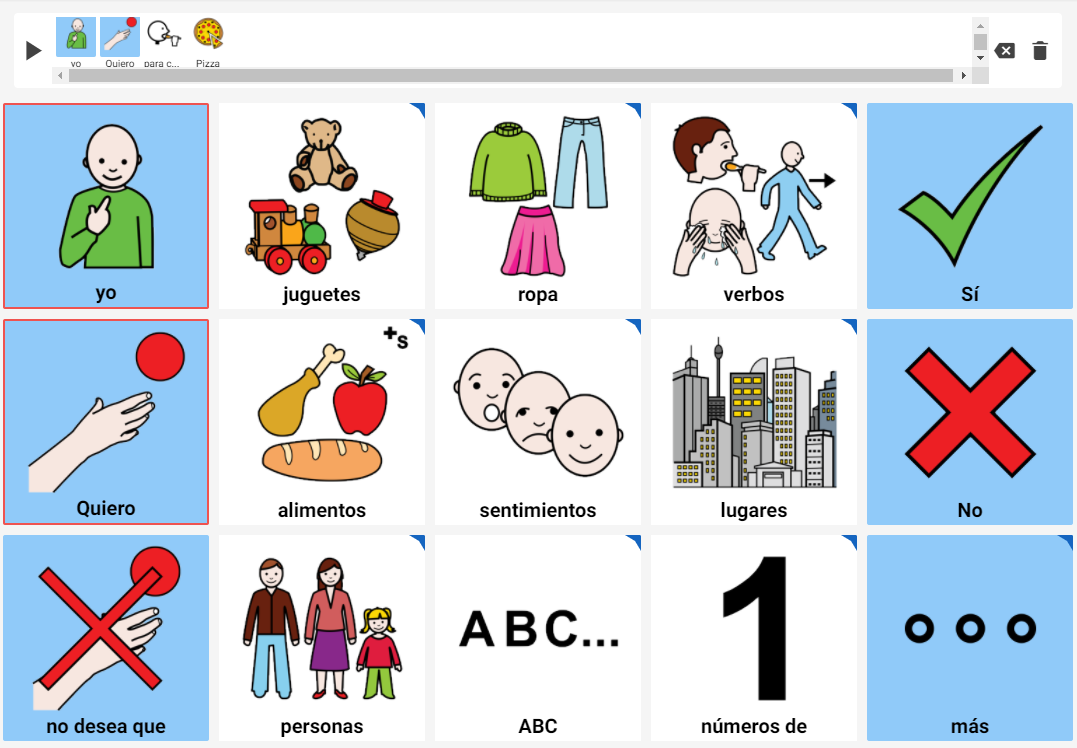
\includegraphics[width=0.7\linewidth]{Imagenes/Bitmap/SymboTalk}
	\caption{Pantalla principal de la aplicación Symbo Talk.}
	\label{fig:symbotalk}
\end{figure}

\newpage
\subsection{LetMe Talk}

LetMe Talk es una aplicación para dispositivos Android e iOS que permite generar frases a partir de pictogramas seleccionados. Tiene un total de 9.000 pictogramas de \textit{ARASAAC} y ofrece la posibilidad de añadir imágenes con un texto descriptivo con la cámara del dispositivo.

\footnote{\url{ https://www.letmetalk.info/es}}
% TODO: \usepackage{graphicx} required
\begin{figure}[h!]
	\centering
	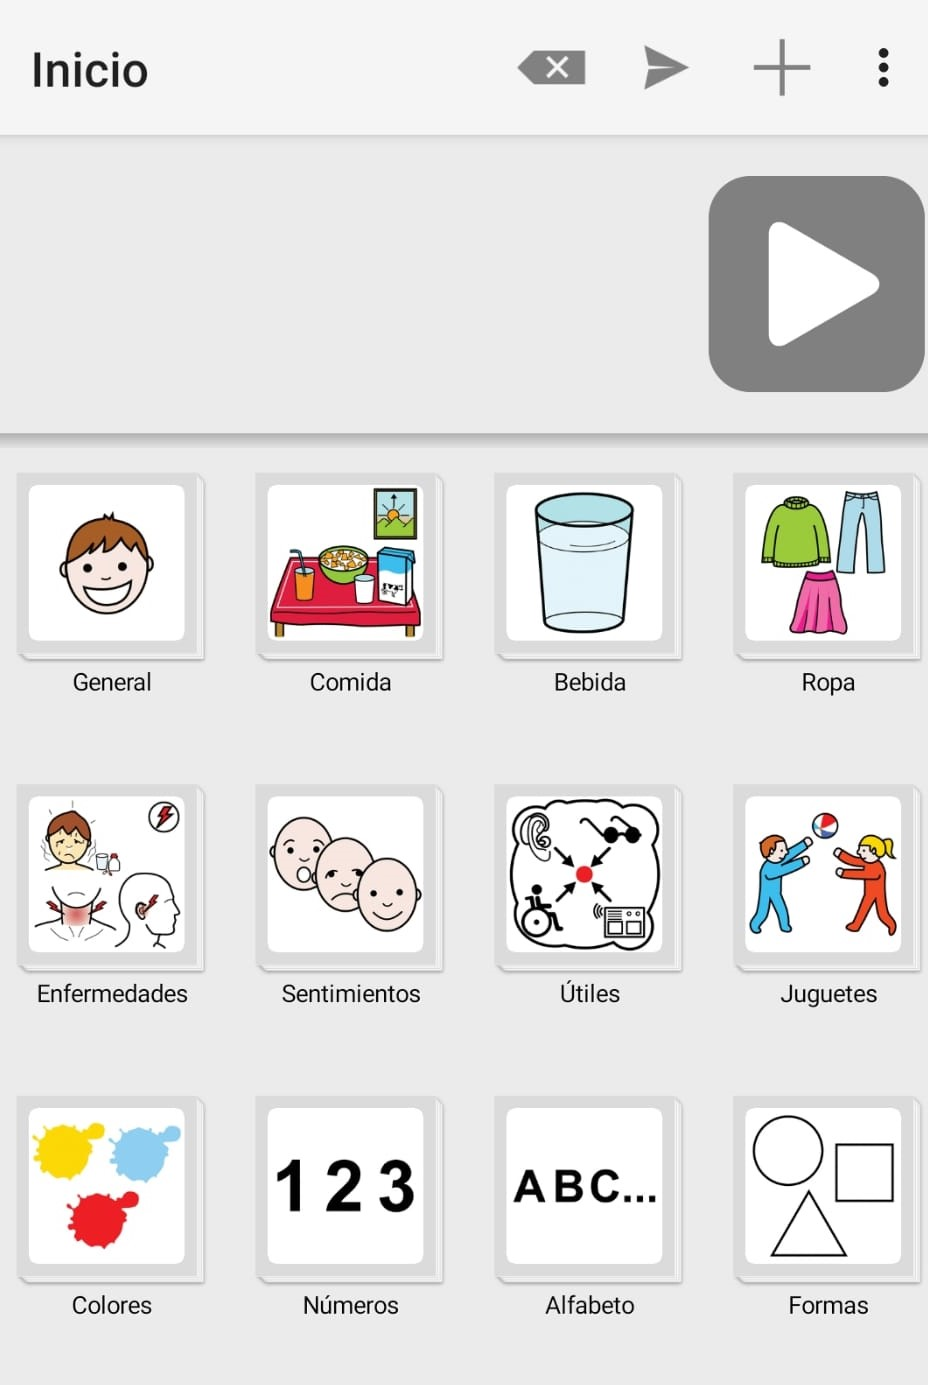
\includegraphics[width=0.7\linewidth]{Imagenes/Bitmap/LetMeTalk}
	\caption{Menú de la aplicación en Android de LetMe Talk.}
	\label{fig:letmetalk}
\end{figure}

\newpage

\section*{Análisis de los resultados}


Puestas todas las herramientas en comparación recopiladas en la Tabla \ref{tab:comparativa}, podemos extraer algunos resultados. Actualmente la mayoría de estas herramientas están disponibles y con una base de datos de pictogramas actualizada. Los más completos o que ofrecen más opciones, están disponibles para ordenadores aunque en dispositivos móviles hay mayor oferta  de aplicaciones, generalmente ofrecen pocas opciones. Además de las aplicaciones de dispositivos, las más actualizadas son las que se pueden acceder en formato web.

Aunque a pesar de todo, el factor determinante es el precio. Las aplicaciones que no son gratuitas suelen tener un precio desorbitado o que muchas familias o docentes no pueden permitirse, por ello que una aplicación sea gratuita es determinante. Respecto a los idiomas, destacan el español y el inglés como idiomas predominantes entre las aplicaciones. 

Como conclusión, creemos que la herramienta que desarrollemos debería cumplir las siguientes características. Debe ser gratuita, disponible desde navegador web, con edición de pictogramas, una base de datos de éstos actualizada y que esté disponible como mínimo en español e inglés. 

\begin{table}[]
	\centering
	\resizebox{14cm}{!} {
		\begin{tabular}{|l|l|l|l|l|l|l|}
			\hline
			
			\textbf{Programas} & \textbf{Disponible} & \textbf{Actualizado} & \textbf{Dispositivos} & \textbf{{\begin{tabular}[c]{@{}l@{}}\\ Permite editar \\ pictogramas \\ \\\end{tabular}}}  & \textbf{Precio} & \textbf{Idiomas} \\  \hline
			
			\textbf{Pictoselector} &Sí  &Sí  &PC y MAC  &Sí &Gratuito &{\begin{tabular}[c]{@{}l@{}}\\ES, EN, DU, FR, \\ PT, IT\\ \\\end{tabular}} \\ \hline
			\textbf{Editor ARASAAC} &Sí  &Sí  &{\begin{tabular}[c]{@{}l@{}}\\PC, MAC, Android, \\ iOS y Web \end{tabular}}  &Sí &Gratuito &{\begin{tabular}[c]{@{}l@{}}\\ES, EN, DU, FR, \\ PT, BZ, IT, RO, \\ PL, CN, AR, RU, \\ BG, CRO, NLD\\ \\\end{tabular}} \\ \hline
			\textbf{Piktoplus} &No  &No  &Android  &No &139€ &{\begin{tabular}[c]{@{}l@{}} \\ES \\ \\ \end{tabular}}\\ \hline
			\textbf{BoardMaker} &Sí  &Sí  &PC y MAC  &No &300€ &{\begin{tabular}[c]{@{}l@{}} \\ES, EN, PT \\ \\\end{tabular}}\\ \hline
			\textbf{Pictar} &Sí  &{\begin{tabular}[c]{@{}l@{}}\\La web no, \\los pictogramas sí\end{tabular}}  &Web  &No &Gratuito &{\begin{tabular}[c]{@{}l@{}} \\ES \\ \\ \end{tabular}}\\ \hline
			\textbf{Pictableros} &Sí  &{\begin{tabular}[c]{@{}l@{}}\\La web no, \\los pictogramas sí\end{tabular}}   &Web  &Sí &Gratuito &{\begin{tabular}[c]{@{}l@{}} \\ES \\ \\ \end{tabular}}\\ \hline
			\textbf{SymboTalk} &Sí  &No  &Web, Android e iOS  &No &Gratuito &{\begin{tabular}[c]{@{}l@{}} \\ES, EN, HEBR \\ \\ \end{tabular}}\\ \hline
			\textbf{LetMeTalk} &Sí  &No  &Android e iOS  &No &Gratuito &{\begin{tabular}[c]{@{}l@{}} \\ES, AR, DE, EN, \\ IT, FR, PL, PT, \\ RU, RO, SW, CN \\ \\\end{tabular}} \\ \hline
			
		\end{tabular}
	}
\caption{\label{tab:comparativa}Tabla comparativa entre los distintos editores de tableros basados en pictogramas}
\end{table}


\include{Capitulos/Tecnologías}
\chapter{Requisitos y diseño}
\label{cap:introduccion}


%\begin{resumen}

%Resumen: En este capítulo se explicarán los prototipos de la aplicación realizados por Alfonso y Jorge (Sección \ref{cap4:diseñoapp}). Después se analizarán ambos prototipos y se definirán los requisitos (Sección \ref{cap4:requisitosapp}) que deberían incluirse en el desarrollo PictUp!.
	
%\end{resumen}

\label{cap1:sec:Motivacion}


\section{Introducción}
De ahora en adelante se referirá a la aplicación como PictUp!. El propósito de la aplicación PictUp! es solventar problemas encontrados en otras aplicaciones similares y combinar las herramientas necesarias para facilitar la creación de materiales pictográficos. Para ello, se han estudiado las características de las distintas aplicaciones vistas en la Sección \ref{cap2:tablacomparativa}. De esta manera, se han seleccionado las funcionalidades imprescindibles para crear un tablero pictográfico y otras atendiendo a las necesidades demandadas por los usuarios. Así se ha podido confeccionar una lista de requisitos iniciales de la aplicación y el motivo de su interés. A continuación, se expondrán las caracterísiticas que debería reunir PictUp!: 


\begin{itemize}
	\item \textbf{Crear tableros con facilidad y precisión}: los pictogramas que se coloquen en el tablero deben de poder alinearse sencillamente. 
	\item \textbf{Utilizar fotografías como material}: algunos usuarios quieren complementar los tableros con imágenes propias que pueden ser más familiares a la persona que se beneficie del tablero. 
	\item \textbf{Agilizar el proceso de búsqueda de pictogramas que sean usados de manera recurrente}: al crear material de manera recurrente puede ser útil contar con los pictogramas más usados para no repetir la misma búsqueda repetidamente. 
	\item \textbf{Añadir interacción a los tableros}: la mayoría de las aplicaciones estudiadas son estáticas, es decir, no permiten una interacción adicional al usuario con el tablero. Algunas aplicaciones aprovechan dicho potencial como Piktoplus (Sección \ref{cap2:pkplus}) mediante los subtableros emergentes o Jocomunico (Sección \ref{cap2:jocomunico}) que permite reproducir la pronunciación del texto asociado a un pictograma.
	
\end{itemize}






\section{Diseño de la aplicación}
\label{cap4:diseñoapp}
Después de probar distintas tecnologías y estudiar la situación actual de los tableros pictográficos, se procedió a bocetar la idea de la aplicación y el formato de la interfaz. Al ser dos integrantes en el proyecto, se realizaron dos bocetos diferentes, a partir de los cuales se concretaron los primeros requisitos y asentaron las bases del proyecto.


\subsection{Prototipo realizado por Alfonso}
\label{cap4:sec:alfonso}
Teniendo en cuenta los requisitos de los usuarios, las aplicaciones existentes y el trabajo futuro de trabajos similares, empezamos a bocetar una primera idea del proyecto.


En la Figura \ref{fig:loginalfonso} podemos ver el boceto de la pantalla de  inicio, la cual estaría compuesta por cuatro secciones bien diferenciadas. \textit{Creación de tablero libre} serviría para crear un tablero donde se pueden colocar pictogramas, texto o figuras. \textit{Creación de actividad} añadiría interacción a los tableros mediante la sucesión de los mismos. Más tarde profundizaremos en esas dos secciones.

% TODO: \usepackage{graphicx} required
\begin{figure}[h!]
	\centering
	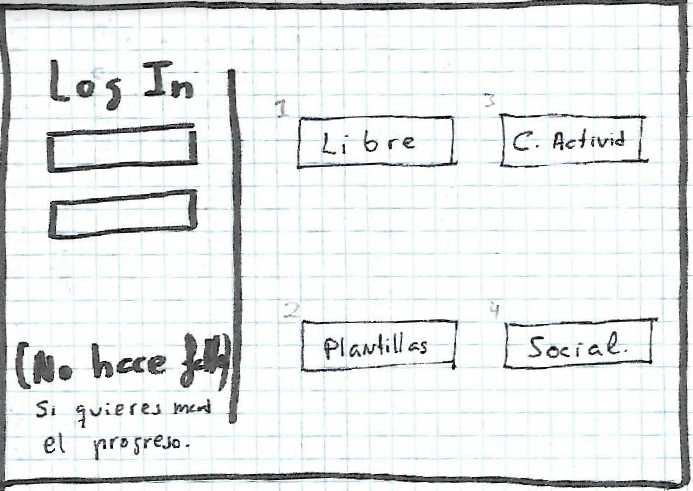
\includegraphics[width=0.7\linewidth]{Imagenes/Bitmap/logInAlfonso}
	\caption{Boceto de pantalla inicial}
	\label{fig:loginalfonso}
\end{figure}

Las \textit{Plantillas} permitirían crear un tablero mediante el uso de una plantilla que cuenta con espacios donde colocar pictogramas. Las plantillas facilitan la creación del material que sigue una misma estructura, pero con contenido diferente. Un ejemplo de ello es la creación de un horario, donde pueden haber decenas de huecos a rellenar y se estructuran generalmente de la misma manera. Al tener una plantilla, el usuario se puede despreocupar de que los elementos queden bien centrados o añadir los días de la semana. En la Figura \ref{fig:inicioalfonso} podemos ver un ejemplo de algunas ideas de plantillas disponibles. 
La sección de \textit{Social} tendría la función de compartir tableros, actividades y plantillas con la comunidad de usuarios. Por último, existe un inicio de sesión opcional para mantener el progreso entre dispositivos.

% TODO: \usepackage{graphicx} required
\begin{figure}[h!]
	\centering
	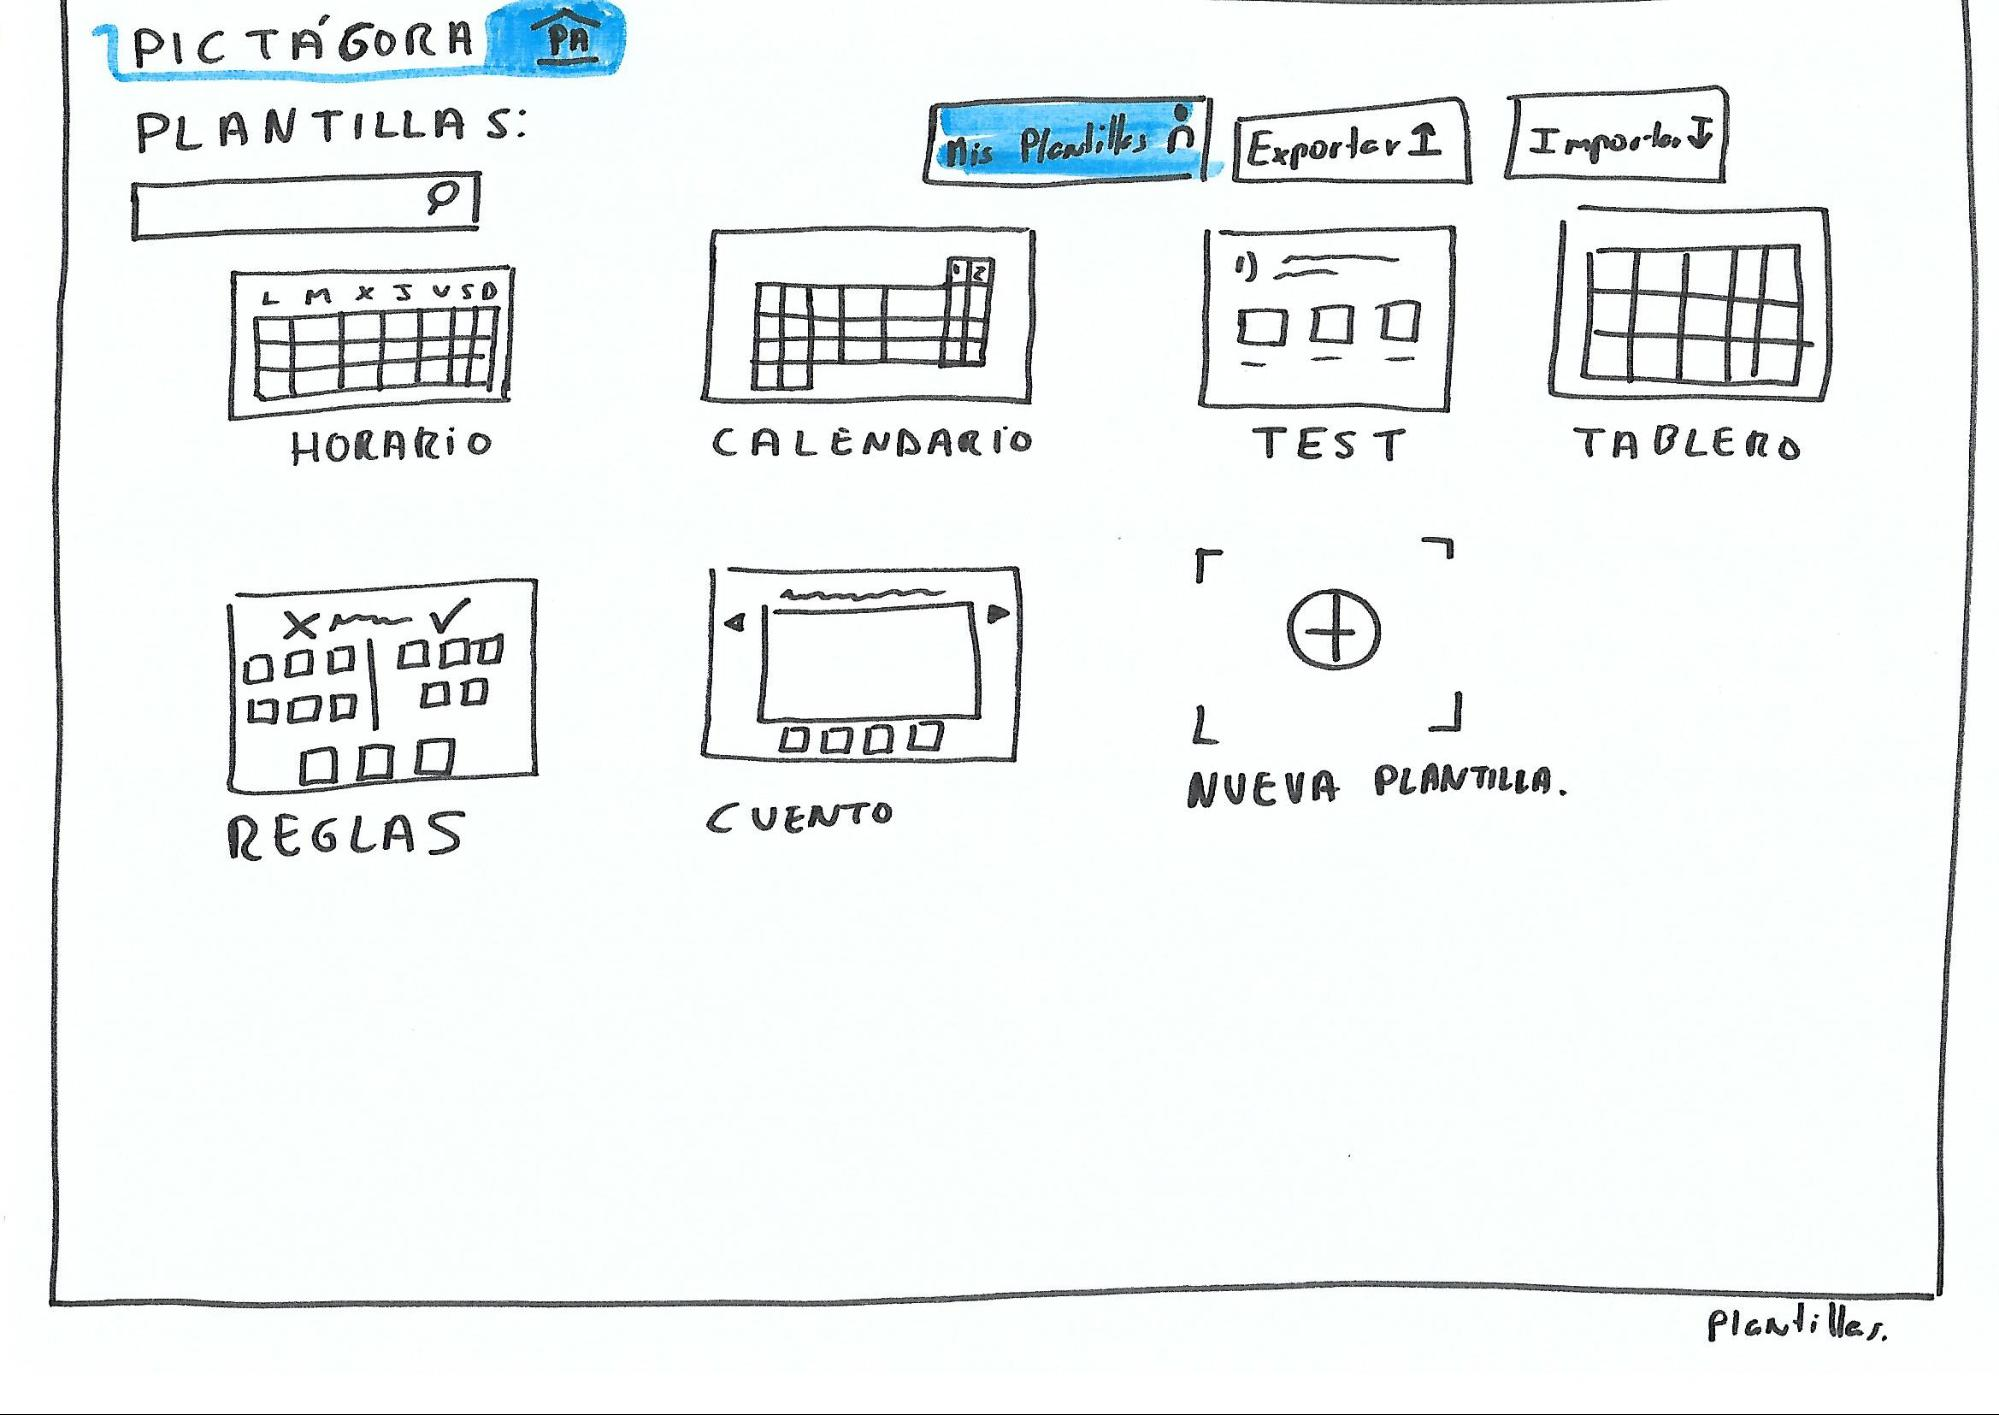
\includegraphics[width=0.7\linewidth]{Imagenes/Bitmap/inicioAlfonso}
	\caption{Boceto pantalla de plantillas}
	\label{fig:inicioalfonso}
\end{figure}


 Si profundizamos en la \textit{Creación de un tablero libre} en la Figura \ref{fig:dibujolibrealfon}, podemos ver los componentes que se pueden colocar sobre el tablero. Éstos son los pictogramas, texto, figuras como flechas o rectángulos y la posibilidad de subir imágenes. También comenzamos a plantear la idea de almacenar colecciones de pictogramas, que almacenan distintos conjuntos de pictogramas que el usuario agrupa según su criterio. Por ejemplo, si un profesor tiene que crear varios tableros respecto a un tema, como “Animales de la granja”, puede ser útil tener una colección con los pictogramas de gallina, cabra, oveja, etc, agilizando el proceso de creación.

% TODO: \usepackage{graphicx} required
\begin{figure}[h!]
	\centering
	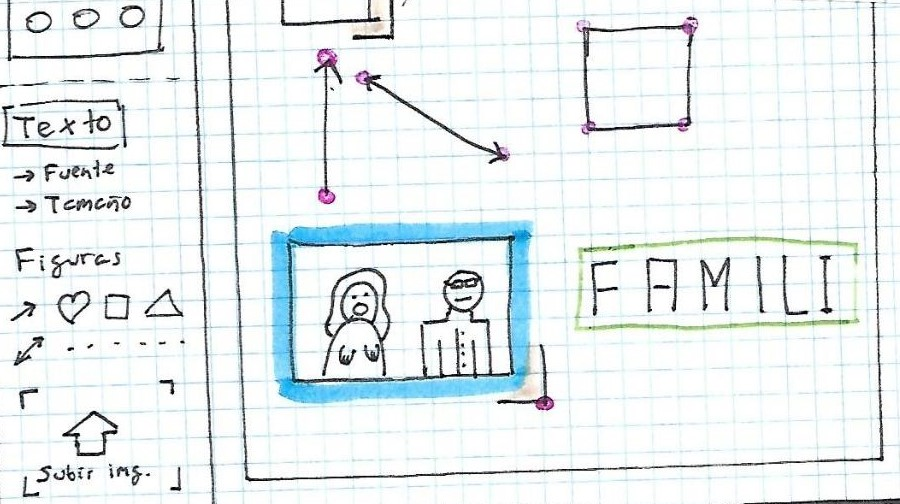
\includegraphics[width=0.7\linewidth]{Imagenes/Bitmap/DibujoLibreAlfon}
	\caption{Boceto pantalla de edición de tableros }
	\label{fig:dibujolibrealfon}
\end{figure}

El apartado de \textit{Creación de actividad} no deja de ser una extensión de creación libre pero con más  componentes que permiten interacción con el usuario para crear distintos tipos de actividad. Estos componentes, que a partir de ahora denominaremos componentes interactivos, son:

\begin{itemize}
	
	\item \textbf{Cajón de pictgramas y espacio picto}: se trata de dos componentes que van ligados entre sí. En primer lugar está el \textit{cajón de picto}, que es un espacio al margen del tablero donde aparecen un conjunto de pictogramas, como se puede ver en la Figura \ref{fig:componentecajon}. Los elementos que aparecen en el cajón pueden  ser desplazados a un \textit{espacio picto}. Este componente es un hueco inicialmente vacío donde puede ser colocado un pictograma como se puede ver también en la Figura \ref{fig:componentecajon}. Ambos componentes son configurables, lo que permite establecer los pictogramas que aparecen en el \textit{cajón de pictogramas}, y los pictogramas que acepta el \textit{espacio picto}. Ambos elementos se beneficiarían de las colecciones, pues son conjuntos de pictogramas establecidos por el usuario.
	
	% TODO: \usepackage{graphicx} required
	\begin{figure}[h!]
		\centering
		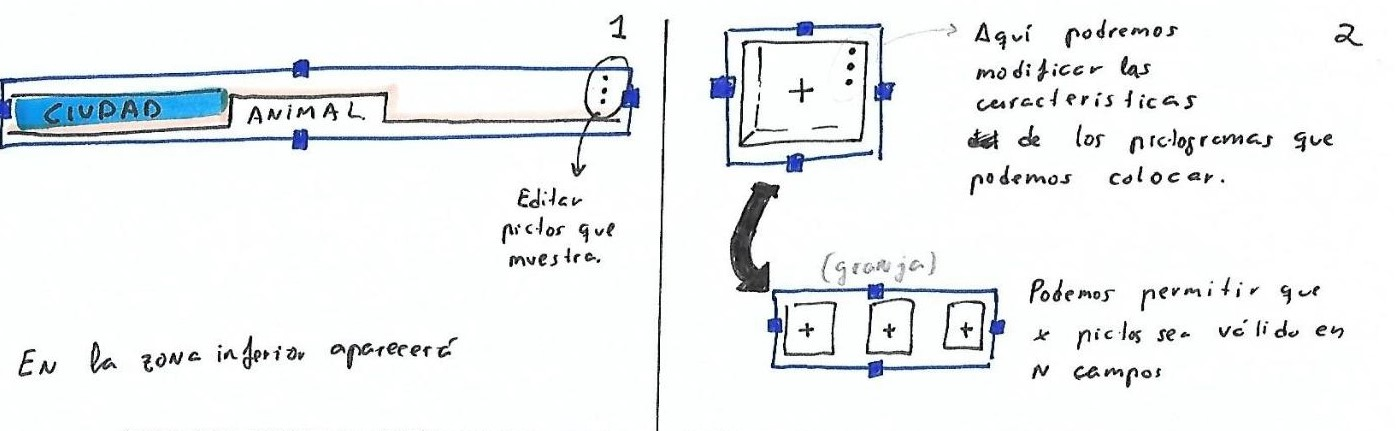
\includegraphics[width=0.7\linewidth]{Imagenes/Bitmap/componenteCajon}
		\caption{Boceto de las componentes canjón de picto y espacio picto.}
		\label{fig:componentecajon}
	\end{figure}
	
	
	Por ejemplo, un cajón de pictogramas podría tener asignado varias colecciones de pictogramas para que aparezcan mezclados. Asimismo, en el \textit{espacio picto} podría ser configurado para únicamente aceptar pictogramas de una de las colecciones o un pictograma concreto. De esta manera podría ser construido con facilidad un ejercicio donde el usuario que interactúe con el tablero pueda arrastrar distintos pictogramas del cajón de pictos a un espacio picto. En la Figura \ref{fig:cajonpictosgranja} se ve el \textit{cajón de pictos} mostrando pictogramas que representan animales de la granja y la selva, junto a unos \textit{espacio pictos} donde colocar los pictos de cada tipo.  El objetivo es dar la máxima flexibilidad al usuario que cree una actividad.
	
	
	% TODO: \usepackage{graphicx} required
	\begin{figure}[h!]
		\centering
		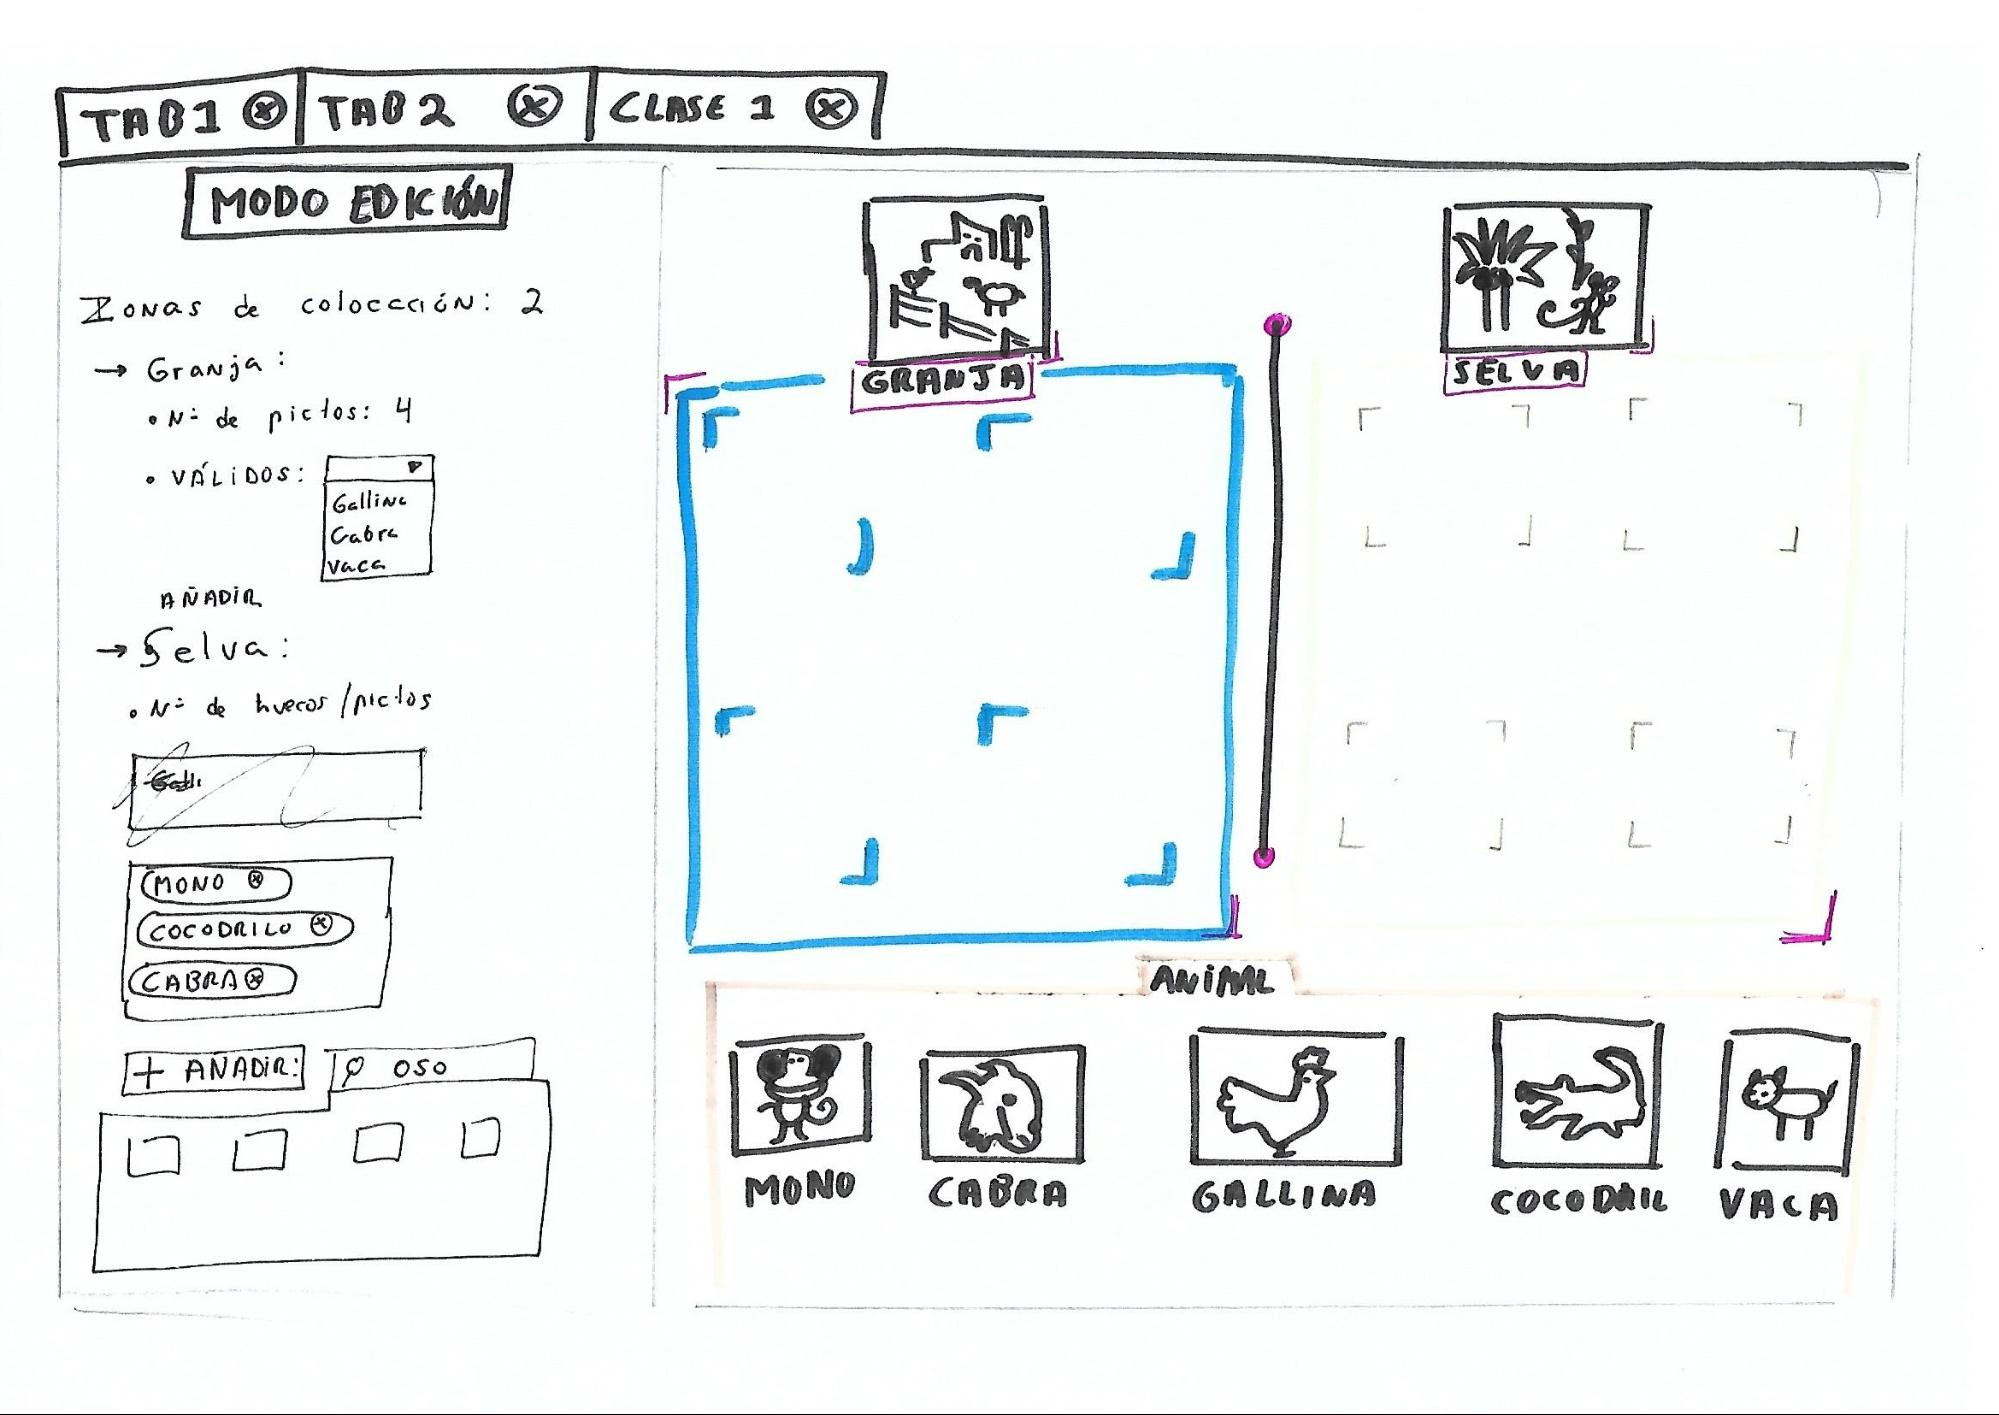
\includegraphics[width=0.9\linewidth]{Imagenes/Bitmap/cajonPictosGranja}
		\caption{Boceto de actividad con cajón de pictos y hueco picto}
		\label{fig:cajonpictosgranja}
	\end{figure}

	\item \textbf{Subtablero}: el componente subtablero permite desplegar un tablero de pictogramas. Los pictogramas que componen dicho tablero pueden venir dados por una colección de pictogramas creada por el usuario o indicarse en el propio componente. Su finalidad es la de añadir más pictogramas en el mismo espacio y agilizar la comunicación. La idea ha sido rescatada de Piktoplus (Sección \ref{cap2:pkplus}) que también permitía crear subtableros.
	
	\item \textbf{Enlace}: permite ligar dos pictogramas diferentes. Está compuesto por dos “piezas” las cuales se asignan a dos pictogramas para ser enlazados. Su finalidad es la de crear actividades como “hacer parejas”.
	
	En la Figura \ref{fig:componenteenla} podemos ver el ejemplo del pictograma hueso y perro, a los cuales se les asignan la misma pieza identificada por un símbolo de pica con fondo verde. El motivo por el que  las piezas tienen una forma y color asociado facilita al usuario que cree la actividad identificar las piezas ya  ligadas. El usuario final al pulsar sobre los pictos permitirá hacer parejas y completar la actividad.
	
	% TODO: \usepackage{graphicx} required
	\begin{figure}[h!]
		\centering
		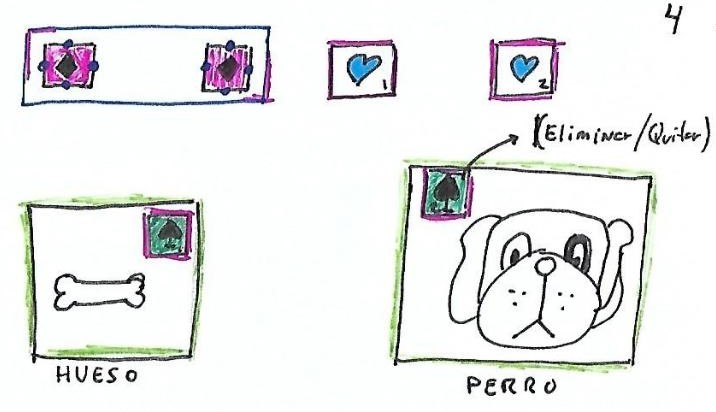
\includegraphics[width=0.7\linewidth]{Imagenes/Bitmap/componenteEnla}
		\caption{Boceto de las piezas que enlazan dos pictogramas al compartir la misma figura}
		\label{fig:componenteenla}
	\end{figure}

	
\end{itemize}

Con todos los tableros creados también es posible crear una actividad de mayor tamaño mediante la secuenciación de tableros. Se podría pasar de uno a las siguientes escenas mediante flechas, como se puede ver en la Figura \ref{fig:cuento}, que está compuesta por una fotografía y algunos pictogramas que la describen. Pero también se podrían intercalar estos tableros con otros que aporten interacción. Por ejemplo podría añadirse un test mediante el cajón de pictos para comprobar si se está comprendiendo la lectura.

% TODO: \usepackage{graphicx} required
\begin{figure}[h!]
	\centering
	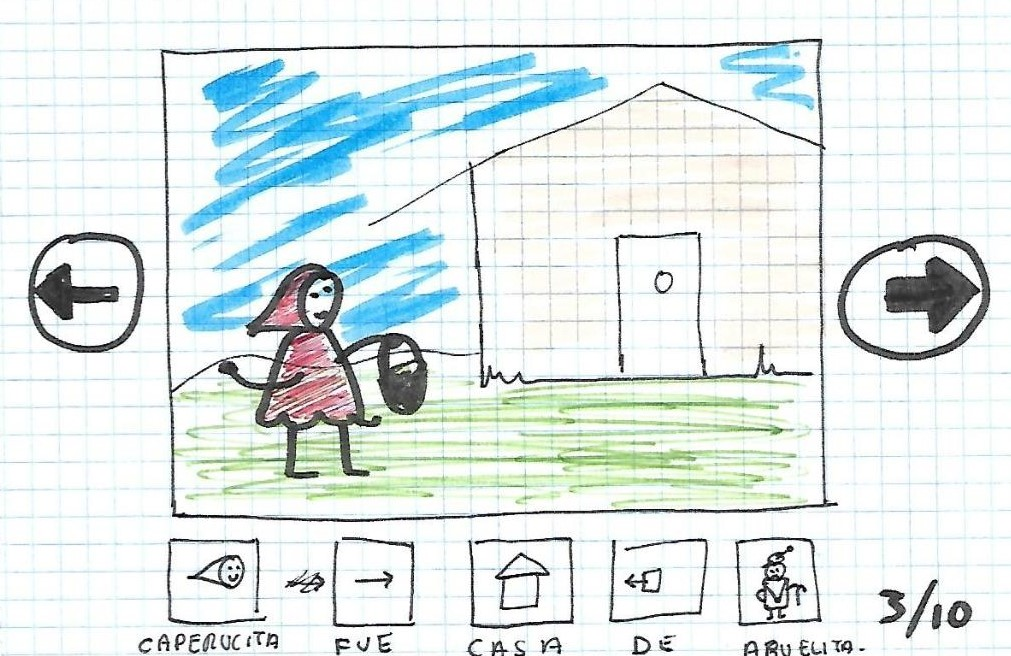
\includegraphics[width=0.7\linewidth]{Imagenes/Bitmap/Cuento}
	\caption{Boceto de una escena de un cuanto, con pictogramas en la zona inferior y botones en los laterales para pasar o retroceder la escena o tablero}
	\label{fig:cuento}
\end{figure}


En la Figura \ref{fig:presentaciontableros} podemos ver cómo se compondrían este tipo de actividades, que resulta muy familiar a la construcción de una presentación de diapositivas.  

% TODO: \usepackage{graphicx} required
\begin{figure}[h!]
	\centering
	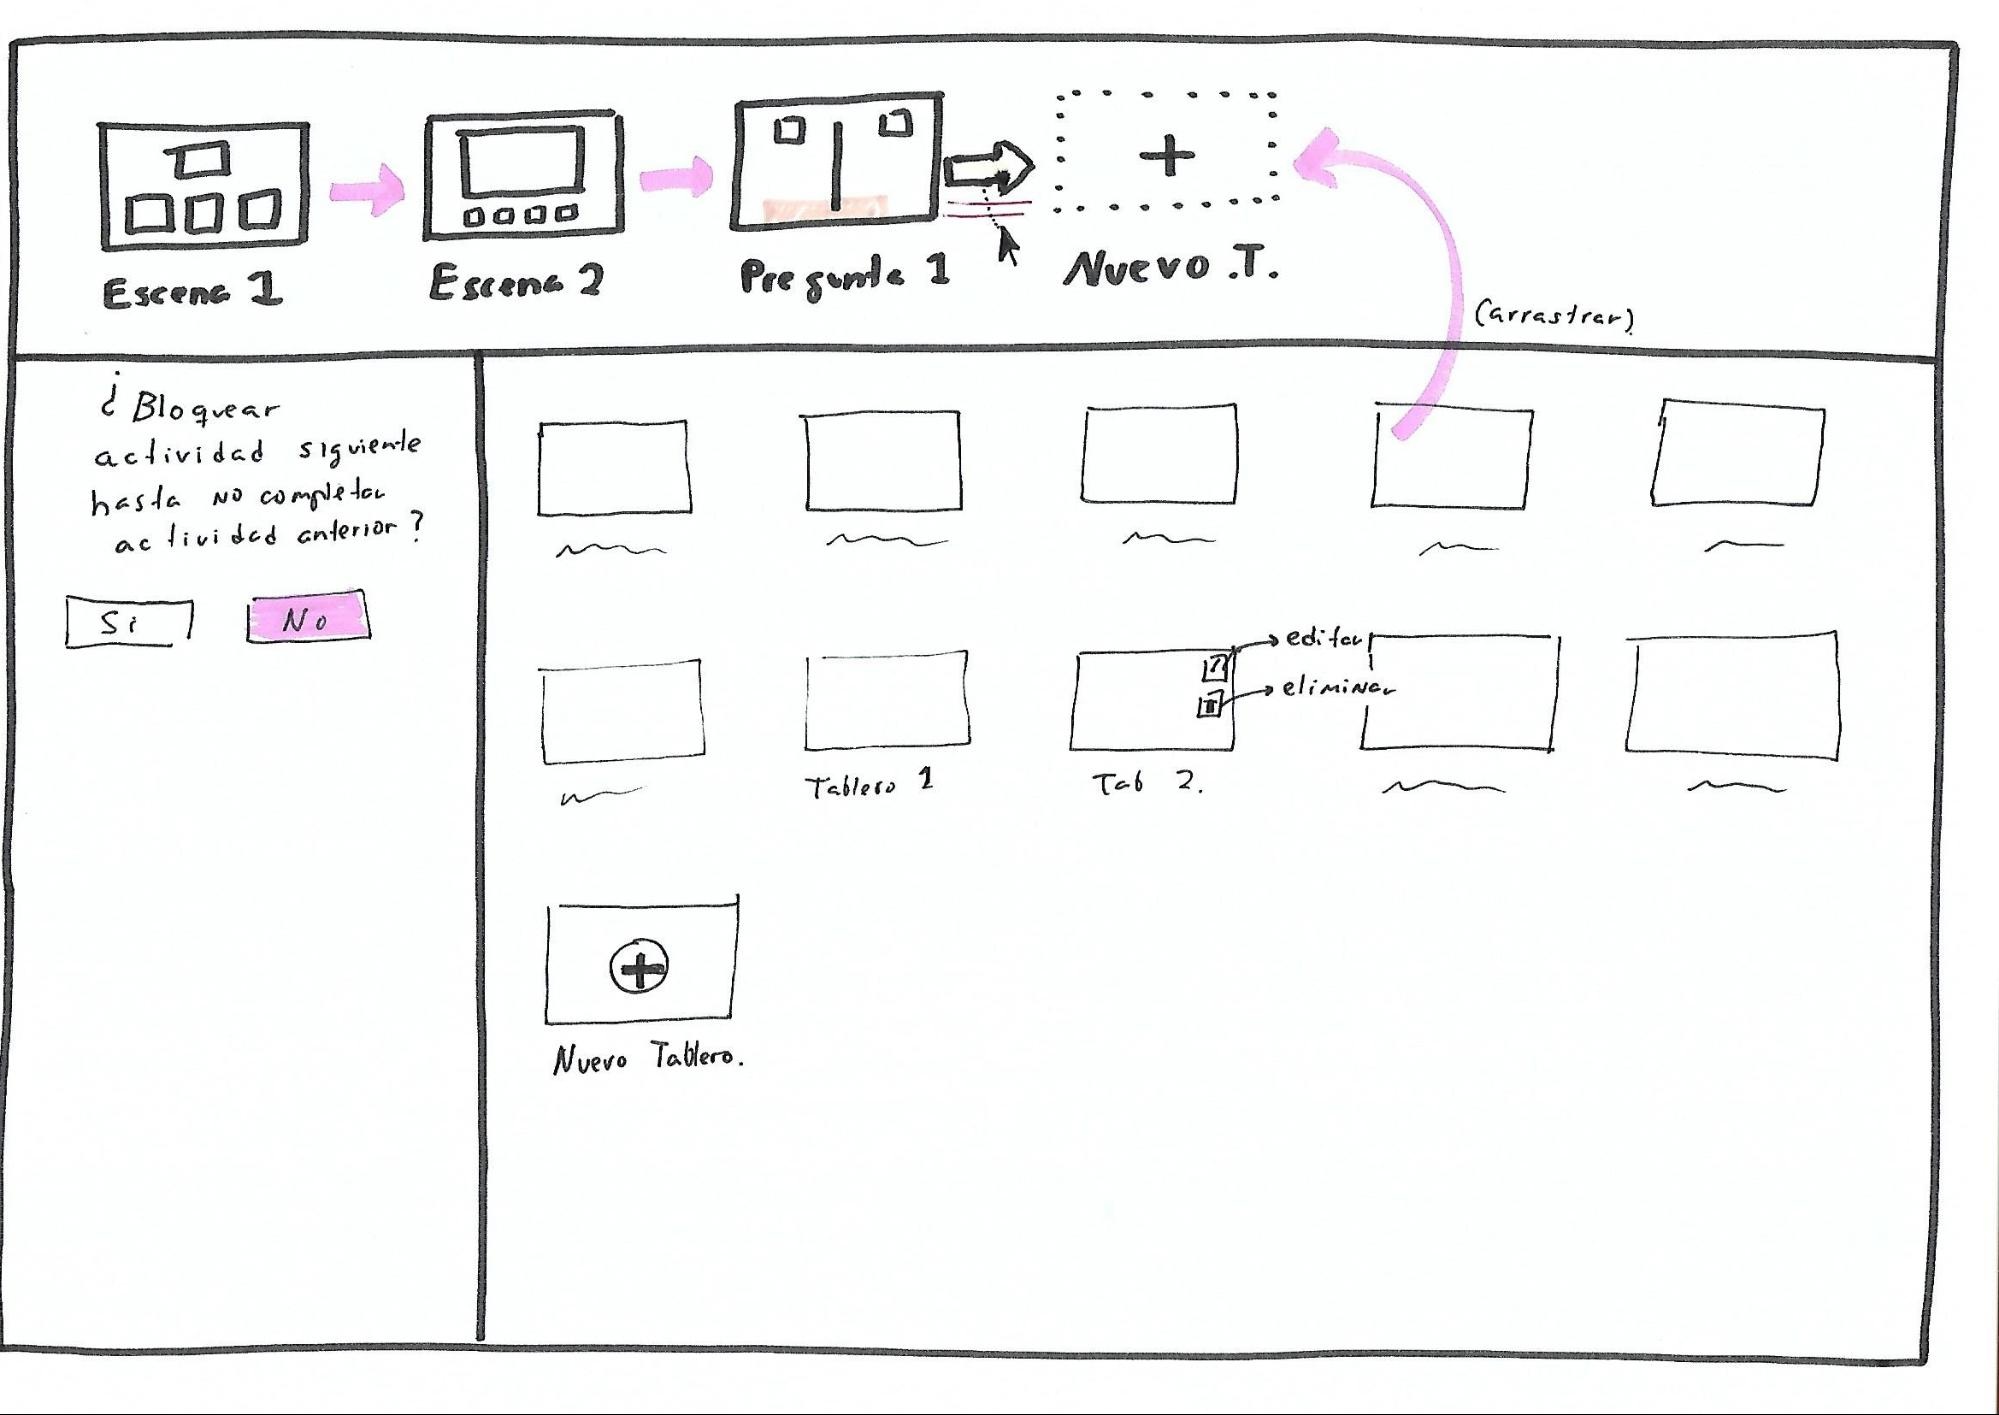
\includegraphics[width=0.7\linewidth]{Imagenes/Bitmap/presentacionTableros}
	\caption{Boceto del compositor de actividades}
	\label{fig:presentaciontableros}
\end{figure}


\subsection{Prototipo realizado por Jorge}
\label{cap4:sec:prototipo}
	
	La pantalla de inicio de la aplicación (ver la Figura \ref{fig:iniciojorge}) está compuesta por cuatro botones. Cada uno de ellos representará una pantalla con distintas funcionalidades. Tambíen podemos ver que en la parte superior de la pantalla tendríamos el nombre de la aplicación a la izquierda, que al pulsarlo volveríamos a esta pantalla, y un selector de idioma en la parte de la derecha. Esta parte sería común en las distintas pantallas de la aplicación.
	
	
% TODO: \usepackage{graphicx} required
\begin{figure}[h!]
	\centering
	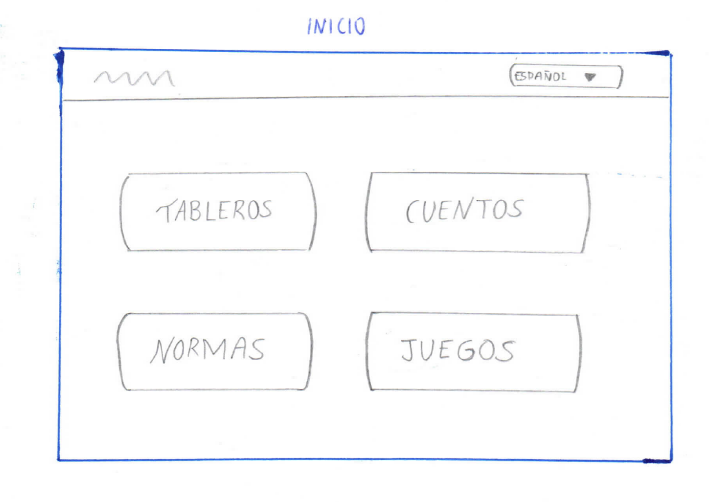
\includegraphics[width=0.7\linewidth]{Imagenes/Bitmap/inicioJorge}
	\caption{Pantalla de inicio con botones que muestran las otras pantallas de la aplicación.}
	\label{fig:iniciojorge}
\end{figure}

	
	En el apartado correspondiente a tableros representado en la Figura \ref{fig:tablerosjorge} podemos diferenciar claramente dos zonas: la parte de la izquierda correspondiente a la personalización del tablero y la parte de la derecha donde se mostraría el tablero que se está editando.
	
	
	En la parte de personalización del tablero podemos ver dos recuadros que englobarían diferentes posibilidades. Las funcionalidades que encontraríamos en el recuadro superior serían las siguientes:
	
	\begin{itemize}
		\item \textbf{Traducir frase}: dada una frase, mostraría toda la secuencia de pictogramas que tuviera ese significado. El botón de insertar que vemos insertaría toda la secuencia de pictogramas en el tablero.
		
		\item \textbf{Búsqueda simple de un pictograma}: dada una palabra concreta mostraría todos los pictogramas que tuvieran ese significado. Al igual que en el apartado anterior también tendríamos un botón de insertar el pictograma deseado al tablero.
	
	\end{itemize}

En el recuadro inferior tendríamos las siguientes opciones:

	\begin{itemize}
	
		\item \textbf{Insertar iconos}: al pulsarlo mostraría un modal con todos los iconos que se pueden añadir al tablero y al pulsar sobre uno de ellos se añadiría al tablero.
		
		\item \textbf{Insertar figuras geométricas}: al igual que con la funcionalidad anterior, al pulsarlo se abriría un modal donde se podrían seleccionar diferentes figuras geométricas para añadirlas al tablero.
		
		\item \textbf{Insertar imágenes}: esta herramienta permitiría al usuario insertar una fotografía que tuviera en su ordenador. A la hora de insertarla en el tablero tendrá las mismas propiedades que un pictograma, la imagen y un texto descriptivo.
		
		\item \textbf{Insertar un campo de texto}: permite añadir un campo en el tablero donde poner textos.
		
		\item \textbf{Editar el tamaño de letra del campo de texto}: esta funcionalidad solo estará disponible si hemos seleccionado un campo de texto en el tablero. Nos permite ajustar el tamaño del texto de un campo específico.
		
		\item \textbf{Editar la fuente del campo de texto}: al igual que con la funcionalidad anterior, deberemos seleccionar qué campo queremos editar. Permite cambiar la fuente del texto por otra.
		
	\end{itemize}
	
	
	En la zona inferior izquierda hay dos botones que permitirían guardar el estado de la página y volver a cargar el estado para posteriormente seguir trabajando con nuestro proyecto.
	
	
	En la zona de la derecha encontramos un tablero donde se insertaría todos los pictogramas, iconos, formas, imágenes y campos de texto. Todos los elementos que se inserten en el tablero podrán ser ampliados de tamaño pulsando sobre una de las esquinas del elemento.
	
	En la parte superior del tablero en sí tendríamos un botón llamado “\textit{Guardar como pdf}” que generaría un archivo con extensión pdf a partir del tablero inferior.
	
	Debajo de dicho tablero encontramos un botón que nos permitiría añadir un nuevo tablero con el que seguir trabajando.
	
	
	
	% TODO: \usepackage{graphicx} required
	\begin{figure}[h!]
		\centering
		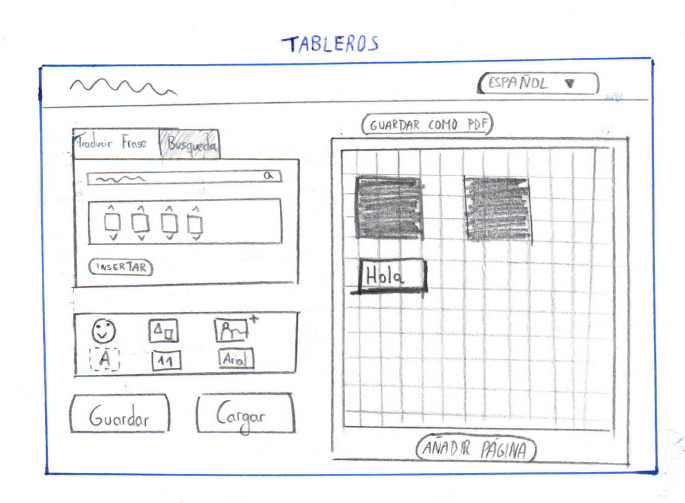
\includegraphics[width=0.7\linewidth]{Imagenes/Bitmap/tablerosJorge}
		\caption{Pantalla de configuración de tablero.}
		\label{fig:tablerosjorge}
	\end{figure}
	
	
	

	Respecto a las pantallas de normas y juegos son relativamente similares, ya que ambas en la parte de la izquierda cuentan con un apartado para la edición y a la derecha el tablero. Las únicas diferencias entre estas pantallas serían los botones que encontramos en el tablero para añadir una nueva norma o sección al cuento. Un ejemplo de la visualización de la pantalla de normas sería la Figura \ref{fig:normasjorge}. Ambas tienen un botón en la parte superior que ofrece la posibilidad de guardar como pdf lo que tenemos en el tablero.
	
	% TODO: \usepackage{graphicx} required
	\begin{figure}[h!]
		\centering
		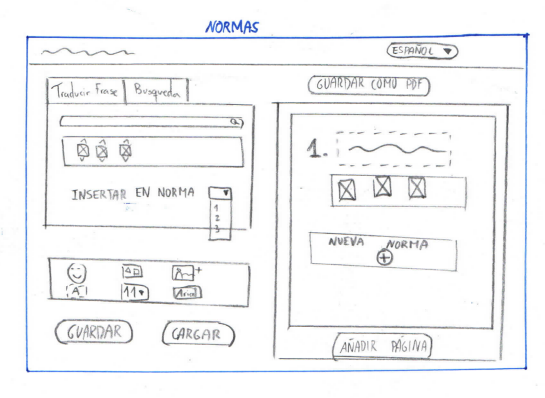
\includegraphics[width=0.7\linewidth]{Imagenes/Bitmap/normasJorge}
		\caption{Pantalla de configuración de normas.}
		\label{fig:normasjorge}
	\end{figure}


	
	Para añadir una norma o una nueva sección en nuestro tablero tendríamos que pulsar sobre el botón “\textit{Nueva norma}” o “\textit{Nueva sección}” y se añadirían dos campos. El primero de ellos estaría numerado y en él se insertaría el texto correspondiente a la norma o a la sección del cuento. El segundo sería un campo en donde poder insertar los pictogramas que queramos que hicieran alusión al campo de texto superior. Además, hay un botón para añadir un nuevo tablero y seguir trabajando.
	

	
	Por último la pantalla de juegos estaría compuesta por dos partes: la primera de ellas sería la configuración del juego y la segunda la ejecución del juego. La pantalla de configuración (ver la Figura \ref{fig:juegosjorge}), al igual que las pantallas vistas anteriormente, cuenta con una sección para la edición y otra para el tablero. En el tablero podremos ver las diferentes secciones que hayamos podido crear y un botón para crear una nueva. Al pulsar sobre este botón se añadirá sobre el tablero una casilla para insertar un pictograma, imagen, icono o figura geométrica, una flecha y un campo de texto. Esto permitirá crear una asociación entre un pictograma y su texto correspondiente para posteriormente ejecutar el juego.
	
	% TODO: \usepackage{graphicx} required
	\begin{figure}[h!]
		\centering
		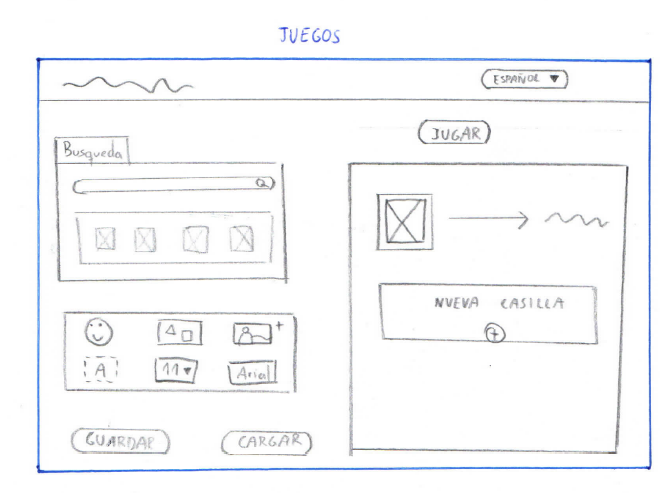
\includegraphics[width=0.7\linewidth]{Imagenes/Bitmap/juegosJorge}
		\caption{Pantalla de configuración de juego.}
		\label{fig:juegosjorge}
	\end{figure}

	Esta pantalla cuenta con dos botones para guardar el estado de la configuración del juego y otro para cargar dicho estado y reanudar el trabajo realizado.
	
	Tras haber creado varias secciones o haber cargado una configuración de juego podremos ejecutar el juego pulsando el botón “Jugar” situado en parte superior de la pantalla. Al pulsarlo nos llevará a una nueva pantalla más simple como se puede ver la Figura \ref{fig:juegojorge}, donde el usuario podrá ver todos los pictogramas que se han seleccionado en la pantalla de configuración y los textos asociados a cada uno de ellos.
	
	Todos los pictogramas seleccionados aparecerán en el recuadro superior de la pantalla. Estos pictogramas se podrán seleccionar y arrastrar a la casilla correspondiente de dicho pictograma. Si al arrastrar un pictograma y soltarlo en una casilla coincide con la norma definida por el usuario, la fecha que une la casilla del pictograma y el texto se pondrá en verde indicando que es correcta esa relación. En caso de que no corresponda el pictograma con el texto, el pictograma volverá a la parte superior donde se encuentran todos los pictogramas, indicando de esta manera que la asociación entre el pictograma y el texto no es la correcta
	 
	

	\begin{figure}[h!]
	\centering
	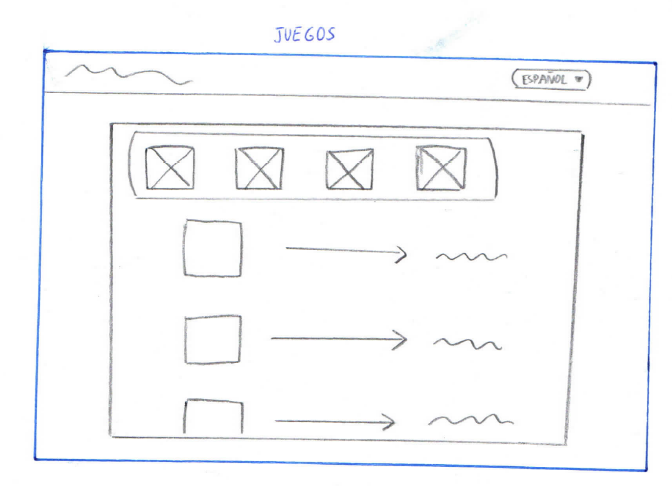
\includegraphics[width=0.7\linewidth]{Imagenes/Bitmap/juegoJorge}
	\caption{Pantalla de juego en ejecución.}
	\label{fig:juegojorge}
	\end{figure}
	

\section{Requisitos de la aplicación}
\label{cap4:requisitosapp}

Tras terminar ambos prototipos, se analizaron para contrastar ideas en común y estudiar posibles funcionalidades y elementos a implementar.

A grandes rasgos, se vio que el prototipo de Alfonso era menos rígido de cara a crear material. Esto es visible en la creación de reglas, cuento o actividades en el prototipo de Jorge, donde solo hay un único formato para cada tipo de material. Por ello se ha optado por ofrecer los componentes al usuario para que este cree el material según su criterio. Los componentes de creación de actividades vistas en el prototipo de Alfonso también ofrecían mayor libertad al crear actividades. 

Un concepto en común entre ambos prototipos es la existencia de una barra de herramientas al lado izquierdo del tablero mediante la cual se añadirían los distintos elementos al tablero. Además, se estableció que debían existir dos tipos de componentes en la aplicación: herramientas y elementos.
A continuación se detallarán las funcionalidades que deberían desempeñar estas componentes. El resto de ideas vistas en ambos prototipos sirvieron para crear una visión general de la posible aplicación, por lo que muchas de estas ideas no fueron desarrolladas.  

\subsection{Herramientas}

En este apartado se incluirán todas aquellas funcionalidades que tras el análisis fueron determinadas como necesarias para desarrollo de la aplicación. Principalmente estas funcionalidades estarán relacionadas con la edición del tablero. Las funcionalidades que se decidió desarrollar fueron:

\begin{itemize}
	\item \textbf{Búsqueda de pictogramas}: esta herramienta permitirá al usuario realizar una búsqueda a partir de una palabra y poder añadir al tablero el pictograma deseado.
	
	\item \textbf{Traducción de frase}: esta herramienta permitirá generar una secuencia de pictogramas asociados a una frase introducida por el usuario y poder añadir esa secuencia al tablero.
	
	\item \textbf{Colecciones}: la herramienta colecciones ofrecen al usuario la opción de poder tener varias agrupaciones de los pictogramas que desee, según su conveniencia. Éstas están compuestas por un nombre que lo identifique y uno o varios pictogramas que el usuario elija según su criterio.
	
	\item \textbf{Importar imágenes}: esta herramienta permite al usuario importar sus imágenes y fotografías y añadirlas al tablero. 
	
	\item \textbf{Añadir texto}: la herramienta de texto permitirá añadir una frase introducida por el usuario al tablero. 
	
	\item \textbf{Añadir icono}: esta herramienta permite añadir al tablero iconos para complementar a los pictogramas, textos o imágenes.
	
	\item \textbf{Importar y exportar}: estas herramientas ayudarán al usuario a poder guardar el estado de la página y poder editarlo posteriormente. 
	
	
\end{itemize}

\subsection{Elementos}


En esta sección analizaremos los principales componentes que se podrán usar en los tableros, como paso previo a su implementación.

Hemos considerado que un elemento es un componente que puede ser añadido al tablero. Distinguiremos dos tipos de componentes: los básicos que no añaden ninguna interacción, y los componentes interactivos. Estos pueden ser ajustados y añadir comportamientos específicos para el usuario que utilice el tablero creado.

\begin{itemize}
	
	
	\item \textbf{Picto}: el elemento picto representa un pictograma junto a su nombre asociado. Cuenta con la opción de poder modificar algunas características del pictograma, como indicar un tiempo verbal. Si el pictograma muestra a una persona, también se puede cambiar el color de pelo y tono de piel.
	
	\item \textbf{Foto}: el elemento foto permite añadir imágenes tanto a partir de una URL como las que suba el propio usuario. Esta ha sido una de las características más demandadas por los usuarios. El permitir añadir fotos abre multitud de posibilidades, como la de poner fotos de la familia, mostrar localizaciones habituales como la cocina e identificar objetos personales que no se representan tan fielmente mediante un pictograma (por ejemplo un juguete específico o la portada de su  libro favorito). Esto facilita al usuario final relacionar conceptos al mostrar figuras que le sean familiares.
	
	\item \textbf{Figuras}: las figuras sirven para ordenar, enfatizar o decorar el tablero. Por ejemplo,  una línea puede ser usada para dividir el espacio de trabajo en secciones, relacionar dos pictogramas o incluso marcar un espacio donde escribir una respuesta si se va a imprimir el tablero. Pese a la simplicidad de las figuras, sus posibilidades son muy amplias según  la creatividad de quien crea el tablero.
	
	\item \textbf{Campos de texto}: Los campos de texto podrán ser insertados en el tablero de la aplicación. Estos campos de texto podrán ser editados permitiendo cambiar el color del texto y aumentar la fuente.
		
\end{itemize}

Hay algunos elementos que tras el análisis de los prototipos decidimos que no iban a aportar lo suficiente en la aplicación o que incrementarían innecesariamente la complejidad. Estos elementos descartados fueron:

\begin{itemize}
	\item\textbf{Pantallas de normas y cuentos predefinidos}: El principal motivo es su falta de flexibilidad, es decir, que si la aplicación no permite crear un cuento o un listado de reglas con sus propias herramientas, tampoco permitirá crear otro tipo de material. Por ello nos hemos decantado por herramientas que ofrecieran más posibilidades al usuario. Otro motivo era que no todos los usuarios querrían por ejemplo que las normas aparecen de una misma manera, como si fuese un listado, por lo que es imprescindible ofrecer la mayor libertad posible al usuario.
	
		
	\item \textbf{Cajón de pictogramas}: El cajón de pictos es un apartado al margen del tablero donde aparecen un conjunto de pictogramas que el usuario debe mover a alguna posición. El hueco donde vayan los pictogramas que se encuentren en el cajón de pictogramas puede ser modificado y aceptar unos u otros. Esto puede ser utilizado como test sencillo de hacer y usar.
	
	\item \textbf{Subtablero}: El subtablero es un componente que a simple vista parece un pictograma pero, al ser pulsado, despliega un tablero que contiene otros pictogramas. Este concepto es originario de Piktoplus pero actualmente no cuenta con soporte y puede ser de utilidad para añadir más pictogramas en el mismo espacio.
	
	\item \textbf{Plantillas}: Tras comentarlo en las reuniones, no se centró mucha atención en este apartado, pues ya estaba muy explorado por la aplicación Pictableros (Sección \ref{cap2:pictableros}).
	
	\item \textbf{Log In}: El principal motivo de su descarte fue el no poder garantizar en un primer momento la total seguridad de los tableros creados.
	Otra de las características del proyecto es la inclusión de imágenes que pudiera subir el usuario, con la responsabilidad añadida de estar manejando imágenes de menores de edad. Estos fueron los motivos por los que optamos por una modalidad sin necesidad de servidor, donde los documentos generados se guardan en el ordenador.
	
	\item \textbf{Selección de idioma}: Fue una idea descartada al principio del desarrollo, en vista de que la gran mayoría de las aplicaciones existentes ofrecían soporte en multitud de idiomas. Pero no se llevó a cabo para centrarnos en otros aspectos de mayor relevancia en el contexto del trabajo.
	
\end{itemize}


\section{Reglas de diseño}
\label{cap4:sec:reglas}
Para asegurar un correcto desarrollo de las distintas funcionalidades que se encuentren en la aplicación, se tendrá en cuenta las ocho reglas de oro de Ben Shneiderman\footnote{\url{https://www.interaction-design.org/literature/article/shneiderman-s-eight-golden-rules-will-help-you-design-better-interfaces}}. A continuación serán enumeradas: 


\begin{itemize}
	
	\item \textbf{Coherencia}: se ha de utilizar los mismos tipos de patrones de diseños en toda la aplicación. Esto incluye los colores, el tipo de letra utilizado, la posición de los botones, etc. Esta regla es de vital importancia ya que facilita al usuario familiarizarse con la interfaz.
	
	\item \textbf{Usabilidad universal}: ha de tenerse en cuenta que la aplicación la pueden utilizar distintos tipos de usuario. A los usuarios más avanzados se les ha de dar la oportunidad de utilizar funciones más complejas frente a los usuarios principiantes. 
	
	\item \textbf{Retroalimentación} informativa: se ha de informar a los usuarios en todo momento de las acciones realizadas de manera visual, por ejemplo mediante cuadros de diálogo.
	
	\item \textbf{Diseñar diálogos para conducir la finalización}: las acciones que requieran de unas ciertas secuencias deberán estar bien organizadas para informar al usuario sobre el momento del proceso en el que se encuentra.  Es importante que tengan una etapa de comienzo, otra de desarrollo y por último una de finalización.
	\item \textbf{Prevenir errores}: se ha de diseñar la interfaz de la aplicación de tal manera que los usuarios cometan el menor número de errores posible. Un ejemplo recurrente es deshabilitar botones o menús. En caso de que ocurra un error se deberá informar al usuario indicando el fallo y las posibles soluciones. 
	
	\item \textbf{Permitir deshacer acciones de forma fácil}: todas las acciones que se realicen en la aplicación deben de ser reversibles. Esto permite a los usuarios realizar acciones sin temor a no poder revertir los cambios realizados.
	
	\item \textbf{Maximizar la sensación de control}:  las acciones no deberían de superar los tres clics. No hay problema si el número es superior siempre y cuando el usuario sepa en todo momento las acciones que está realizando. 
	
	\item \textbf{Reducir la carga de memoria a corto plazo}: es importante que la información que se muestre al usuario sea breve y concisa. Además también es importante agrupar todas aquellas funcionalidades similares para reducir la carga de memoria del usuario.
	
\end{itemize}



\chapter{PictUp! Arquitectura e implementación}
\label{cap:arquitectura}


%\begin{resumen} 
%La arquitectura de la aplicación (Sección \ref{cap5:arquitectura}), funcionamiento de la cuadrícula (Sección \ref{cap5:cuadricula} ), el desarrollo de las funcionalidades implementadas (Secciones de \ref{cap5:buscador} a \ref{cap5:descargar}), las funcionalidades no implementadas (Sección \ref{cap5:noimplementadas} ) y el despliegue (Sección \ref{cap5:despliegue}). Por último se explicará cómo se ha organizado el desarrollo y control de versiones de PictUp! (Sección \ref{cap5:controlversiones} ) 

%\end{resumen}

\section{Introducción}

Una vez especificados las características y requisitos a implementar, se pudo empezar a desarrollar la arquitectura de la aplicación y la implementación de dichas características. Desde un primer momento, se determinó que la aplicación tendrá una barra de herramientas donde se incluirán distintas funcionalidades como buscar pictogramas o realizar traducción de frases. Asimismo se incluirá una cuadrícula donde se podrán poner sobre ella los distintos elementos de los materiales pictográficos. El conjunto de estas funcionalidades permitirá crear tableros pictográficos. A continuación se explicará la jerarquía utilizada en la aplicación, las funcionalidades y los ítems disponibles. 

\section{Arquitectura}
\label{cap5:arquitectura}

La arquitectura de PictUp! puede distinguirse a dos niveles. A nivel interno se especificará la arquitectura de un componente de React, pues todos ellos cuentan con un diseño similar. A nivel externo, se especificará cómo las distintas componentes desarrolladas interactúan entre ellas y se verá un esquema de la jerarquía de éstas. 


\subsection{Arquitectura interna}

La aplicación está compuesta principalmente por componentes\footnote{\url{https://reactjs.org/docs/react-component.html\#gatsby-focus-wrapper}} de React, los cuales son clases que deben contar obligatoriamente con un método \texttt{render()} y de manera opcional puede contar con el objeto \texttt{state}\footnote{\url{https://reactjs.org/docs/faq-state.html\#what-does-setstate-do}}. El objeto \texttt{state} permite almacenar distintas variables. La principal característica de este objeto es que al actualizar el valor de cualquiera de sus variables definidas en su interior, el componente vuelve a renderizarse. Para actualizar el valor de cualquier variable del \texttt{state}, ha de realizarse mediante el método \texttt{setState()}. Este método se realiza de manera asíncrona, por lo que los valores de \texttt{state} generalmente van ligados a datos que serán mostrados en el método renderización. De esta manera,  \texttt{state} será de gran ayuda para actualizar la interfaz con la que interactúa el usuario. 
Los componentes pueden tener variables fuera del objeto \texttt{state} si no se va a utilizar para la renderización.  


El método \texttt{render()}\footnote{\url{https://es.reactjs.org/docs/rendering-elements.html }} se encarga de renderizar el html del componente. Dentro del render se podrán incluir los atributos que se hayan definido en el \texttt{state} u otros elementos como botones, selectores o campos de texto. 
La característica principal que ofrece este método de React es que si se modifica un atributo del \texttt{state} del componente, automáticamente se mostrará en el navegador en nuevo valor que haya tomado. Otra característica que ofrece React es poder llamar desde el render a funciones externas dentro del componente que se encargan de devolver el fragmento html deseado. Esto sirve para organizar mejor el contenido y crear render condicionales, es decir, mostrar un contenido u otro en función de los valores que tomen un atributo del \texttt{state}.
Además también se puede incluir dentro de la función render otros componentes de React, que pasará a ser el componente hija que puede recibir parámetros de entrada o salida mediante \texttt{props}. Las \texttt{props} son atributos de React que permiten enviar información entre componentes padres e hijos. Para acceder a los parámetros enviados desde el componente padre se hará utilizando \texttt{this.props}\footnote{\url{https://es.reactjs.org/docs/components-and-props.html }}.

\subsection{Arquitectura externa}

Una vez vista la estructura de un componente, se puede ver en la Figura \ref{fig:pantallaprincipal} la pantalla principal de PictUp!, la cual está compuesta por multitud de componentes. Estos son agrupados y gestionados mediante el componente Main. Como se puede ver en dicha Figura, se pueden distinguir varios apartados bien diferenciados: 

% TODO: \usepackage{graphicx} required
\begin{figure}[h!]
	\centering
	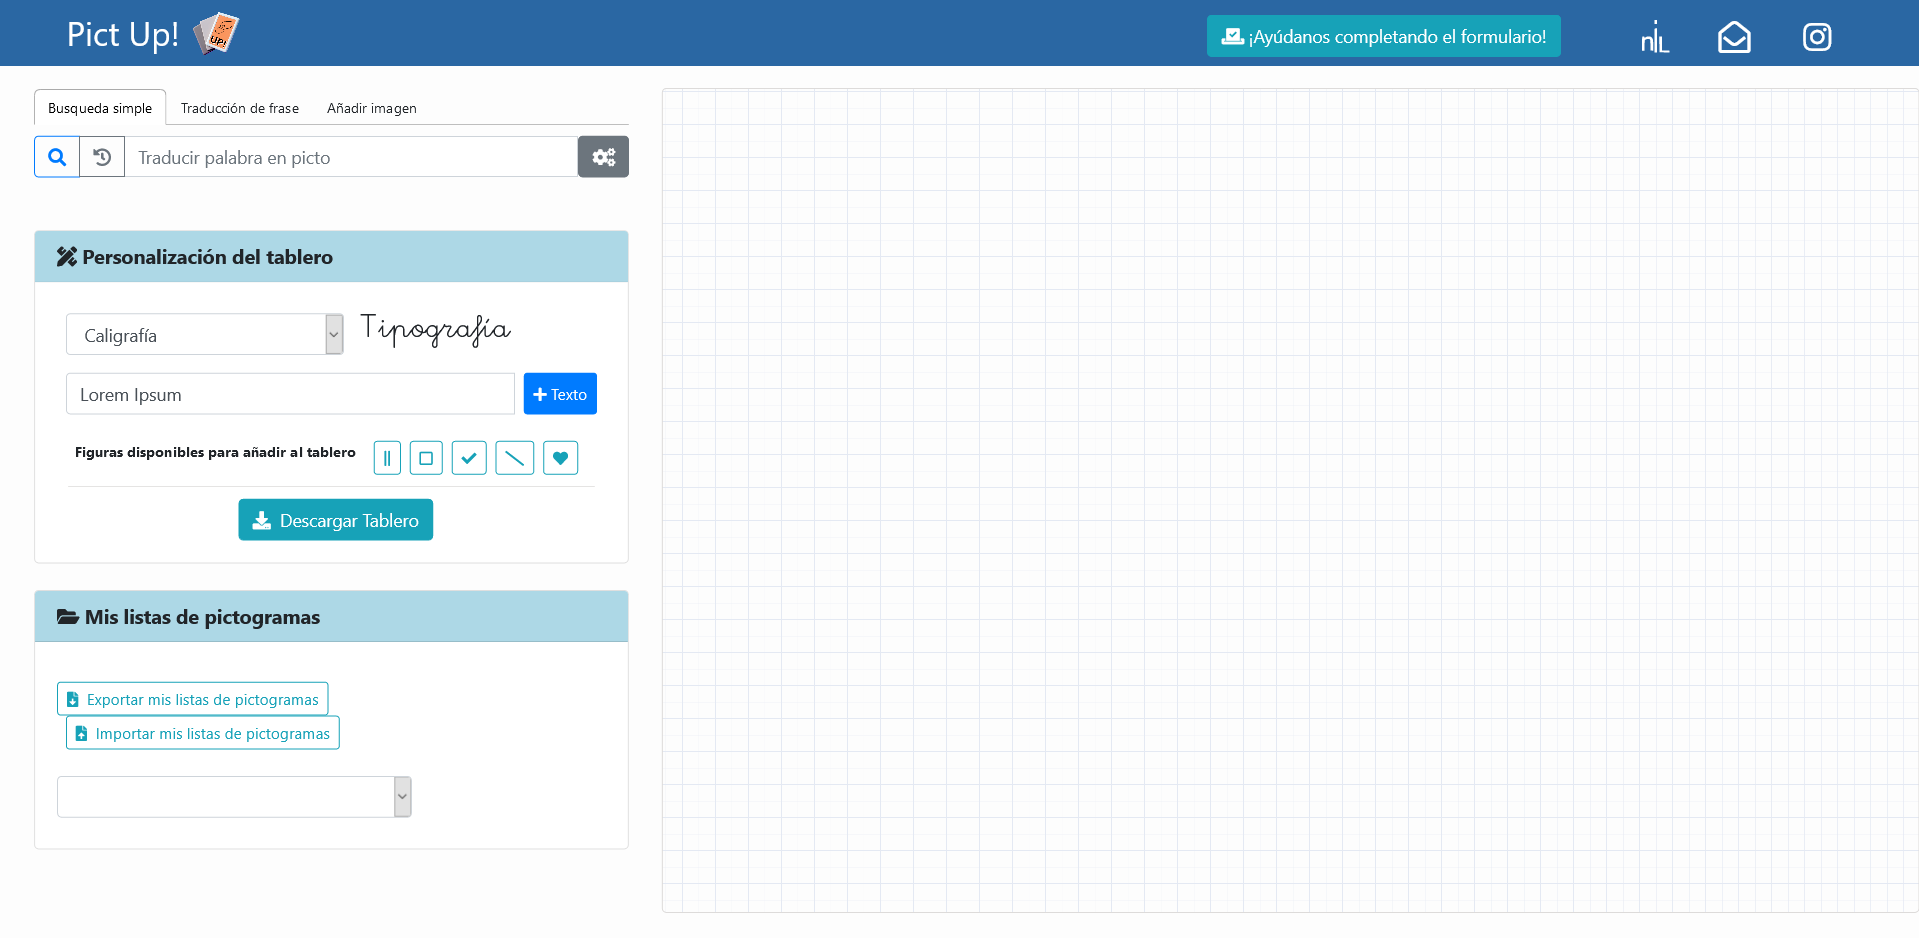
\includegraphics[width=\linewidth]{Imagenes/Bitmap/pantallaprincipal}
	\caption{Vista inicial de PictUp!
	}
	\label{fig:pantallaprincipal}
\end{figure}

\begin{itemize}
	\item \textbf{Navbar}: se encuentra en la zona superior y en ella vemos el nombre de la aplicación junto con su imagen. También se incluye información de contacto.
	
	
	\item \textbf{Barra de Herramientas}: en la zona izquierda de la aplicación se agrupan todas las herramientas disponibles. 
	Estas son componentes que ofrecen una interfaz al usuario para añadir elementos a la cuadrícula. Algunas de estas herramientas cuentan con pantallas auxiliares en forma de modal, como es el caso de búsqueda de pictogramas o la función de descargar tablero. Cada una de las herramientas pueden retornar elementos con representación en la cuadrícula, los cuales serán denominados ítems. La información asociada a cada uno de estos ítems serán almacenados en el \texttt{state} de Main dependiendo de su tipo.
	
	\item \textbf{Tablero}: es el componente que mayor espacio abarca de la página, siendo la zona donde se desplazarán los elementos generados por las herramientas. El tablero se muestra en forma de cuadrícula. Sobre ésta se colocarán los ítems que tenga almacenados Main en su \texttt{state}.  Como se puede ver en la Figura \ref{fig:items} existen distintos tipos de ítem, como pictograma, texto o icono. Cada ítem está adecuado en función del tipo de contenido que se vaya a mostrar. Asimismo, los ítems cuentan con funcionalidades que les permiten cambiar sus propiedades. Por ejemplo, el que representa texto podrá modificar el tamaño de letra y contenido.  
	
\end{itemize}


	

% TODO: \usepackage{graphicx} required
\begin{figure}[h!]
	\centering
	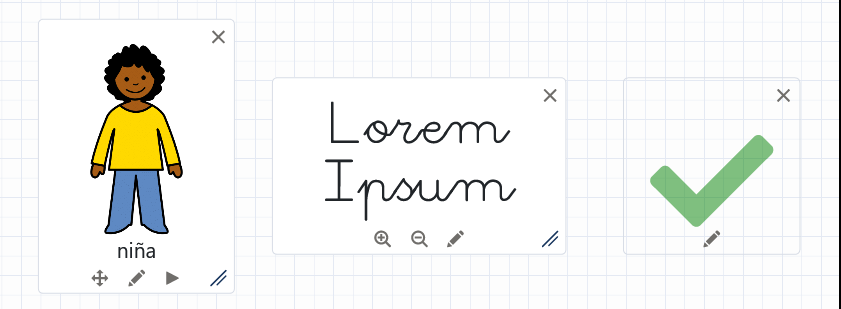
\includegraphics[width=0.7\linewidth]{Imagenes/Bitmap/items}
	\caption{Ejemplos de Ítems}
	\label{fig:items}
\end{figure}
	

Para esquematizar cómo interactúan la distintas componentes, la Figura \ref{fig:diagramaarquitectura} representa cómo se estructura la arquitectura externa.

% TODO: \usepackage{graphicx} required
\begin{figure}[h!]
	\centering
	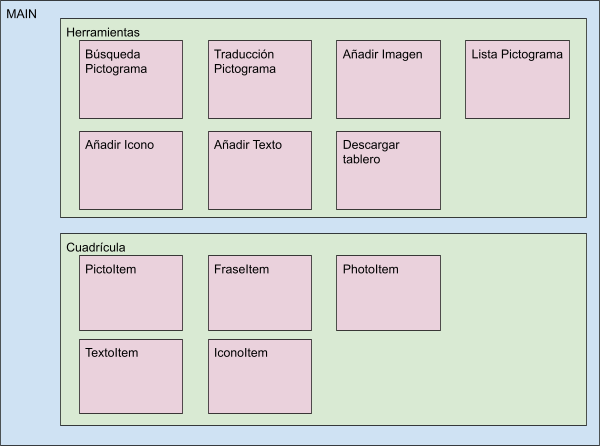
\includegraphics[width=\linewidth]{Imagenes/Bitmap/diagramaarquitectura}
	\caption{Diagrama de los componentes de la aplicación.}
	\label{fig:diagramaarquitectura}
\end{figure}


\subsection{Cuadrícula}
\label{cap5:cuadricula}

En esta sección se explicará el funcionamiento en detalle de la cuadrícula. Para facilitar la tarea de desplazar elementos en un espacio, el proyecto de la cuadrícula fue clonado del proyecto  \textit{dnd-a11y-patterns}\footnote{\url{https://github.com/salesforce-ux/dnd-a11y-patterns}} que contaba con componentes que permitían desplazarse de distintas maneras. Cuenta con una licencia BSD 3-Clause que permite libertad de modificación y distribución.


El empezar desde este proyecto facilitó el  tratamiento de eventos de desplazamiento (Drag and Drop), los cuales iban a ser de gran importancia para mover los distintos ítems de la aplicación. Además de gestionar estos eventos, cuenta con muchos parámetros que han sido modificados, como el ancho y alto inicial de cada ítem o la posibilidad de mantener la proporción de un ítem al ser redimensionado.

El componente de cuadrícula o canvas es una cuadrícula de la cual se puede modificar su tamaño mediante la cantidad de filas y columnas y el intervalo en píxeles entre estas. El tamaño de la cuadrícula fue ajustado para que abarque el mayor ancho y alto posible teniendo en cuenta el espacio reservado para la barra de herramientas. Sobre esta componente canvas se colocarán otros componentes, que serán los ítems. 

Los ítems son elementos que se pueden colocar sobre la cuadrícula de la aplicación y permiten ser desplazados y redimensionados. Al haber distintos tipos de ítems cada uno de ellos mostrará el contenido de distintas maneras. Por ejemplo, los PictoItem tendrán en su interior una imagen del pictograma mientras que el TextoItem simplemente tendrá un texto. Dado que los ítems se encuentran dentro de la clase cuadrícula, reciben atributos tales como el intervalo de la cuadrícula. Esto permitirá a los ítems desplazarse en función de dicho intervalo, ayudando al usuario a mover y redimensionar los ítems con mayor precisión. Al existir distintos elementos que se pueden colocar en la cuadrícula (pictos, fotos, figuras, texto, etc), cada uno cuenta con su propio  ítem que los representa (PictoItem, FotoItem, FigureItem, etc).


Cada ítem cuenta con un renderizado y funcionalidades adecuadas para cada elemento. La mayoría de estos ítems tienen en común los botones visibles en la Figura \ref{fig:botonesitem}, como desplazar y redimensionar (los cuales habilitan la utilización de las teclas del teclado para realizar estas dos acciones con una mayor precisión), y otro botón en la esquina superior derecha para eliminar el pictograma de la cuadrícula. Cuando se pulsa, se envía al componente padre el item seleccionado para ser eliminado de la lista donde se encuentre.

% TODO: \usepackage{graphicx} required
\begin{figure}[h!]
	\centering
	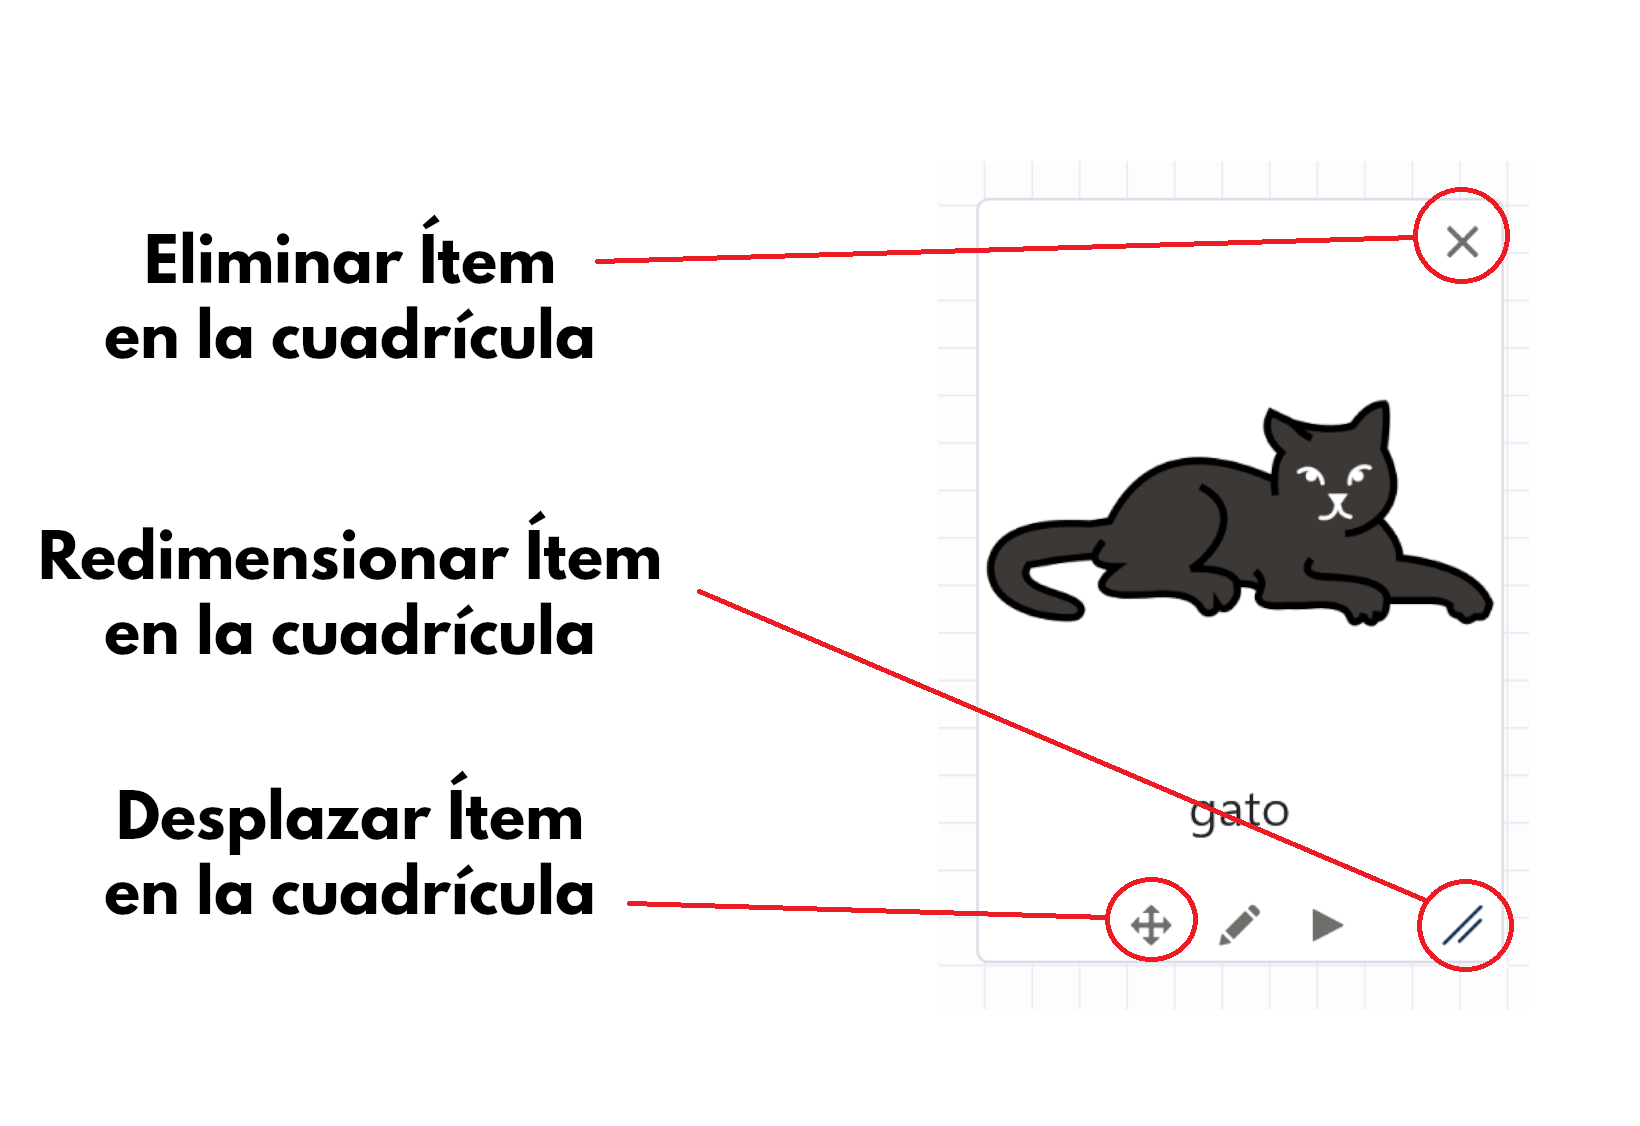
\includegraphics[width=0.7\linewidth]{Imagenes/Bitmap/botonesItem}
	\caption{Ejemplo de botones de redimensión y desplazamiento.}
	\label{fig:botonesitem}
\end{figure}


Una vez explicado cómo funciona a nivel interno la aplicación, se procederá a explicar el funcionamiento de las distintas herramientas y las posibilidades que ofrecen. En caso de que una herramienta cree un ítem en la cuadrícula, se explicarán sus opciones y posibilidades. Asimismo se especificarán las reglas de diseño utilizadas en cada una de ellas (ver Sección \ref{cap5:reglasBusqueda}).



%\section*{Funcionalidades de PictUp!}

%A continuación se explicarán las funcionalidades que podemos encontrar en la aplicación, su representación en caso de contar con un item y que reglas de diseño son utilizadas.

\section{Buscador de pictogramas}
\label{cap5:buscador}
El buscador de pictogramas es la herramienta que muestra los distintos pictogramas que se asocian a una palabra mediante la API de \textit{ARASAAC}. Como se puede ver en la Figura \ref{fig:buscarpicto2}, el componente, aparte de contar con el buscador identificado mediante el icono de la lupa, también tiene un historial que almacena los pictogramas recientemente añadidos asociado al icono del reloj. Además, a la derecha del buscador se encuentra la opción de preajuste de pictogramas identificado con el icono de los engranajes. Estas dos opciones son muy convenientes de cara a añadir un pictograma al tablero. 


% TODO: \usepackage{graphicx} required
\begin{figure}[h!]
	\centering
	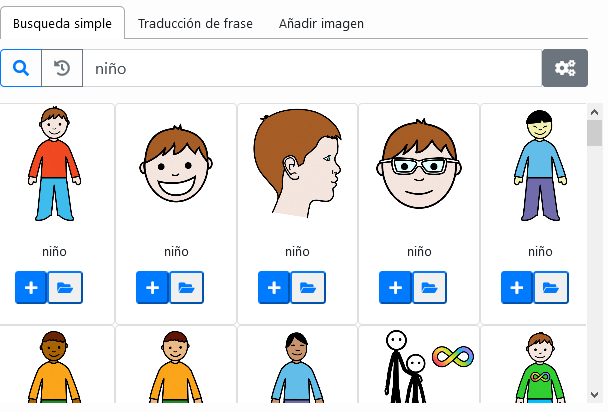
\includegraphics[width=0.7\linewidth]{Imagenes/Bitmap/buscarPicto2}
	\caption{Vista del componente de búsqueda de pictogramas}
	\label{fig:buscarpicto2}
\end{figure}


Para empezar se va a explicar cómo está estructurado el componente de búsqueda de pictogramas. En la variable \texttt{state} del componente se almacenará:

\begin{itemize}
	\item La palabra de la que se quiere obtener sus pictogramas.
	\item Los pictogramas encontrados por la consulta.
	\item El preajuste de los pictos, donde se especifica cómo se van a mostrar los pictogramas.
	\item Flags de control, para indicar si se ha completado la búsqueda, está abierto el modal, o si se ha seleccionado el historial.     
\end{itemize}

Respecto a las funciones que abarca el componente, se pueden distinguir tres tipos: las que realizan las peticiones a la API de ARASAAC, las que gestionan los resultados de las peticiones y dos métodos de renderización. El primer método se encargará de mostrar la barra de búsqueda, que cuenta con los botones mencionados anteriormente (buscar, historial, preajuste de pictogramas) que llamarán a sus funciones asociadas. El segundo método de renderización recibe como parámetro de entrada una lista de pictogramas y los mostrará junto a los botones para añadirlos a la cuadrícula o lista de pictogramas. A continuación se explicará el funcionamiento de estas funcionalidades. 


\subsection{Búsqueda}

Al pulsar sobre el icono de la lupa o pulsar intro se lanza la consulta a la API de ARASAAC por el método \texttt{bestSearch} mediante Fetch\footnote{\url{https://developer.mozilla.org/es/docs/Web/API/Fetch_API/Using_Fetch}}. El fetching puede realizar y recibir peticiones en JavaScript de manera asíncrona de manera sencilla. De esta manera, hasta no recibir una respuesta en forma de JSON con la lista de pictogramas, no se enviará al método de renderización de pictogramas. 

Cuando llegue dicha lista a este método, será cuando se use el preajuste para que la apariencia de los pictogramas sea de acuerdo a lo marcado por el usuario. En la Sección \ref{preajuste} se explica en detalle cómo se obtiene y modifica la URL que se muestra. Con la URL creada, se mostrarán los pictogramas devueltos por la API. El método de renderización añade a cada pictograma dos botones: añadir a la cuadrícula y guardar en una lista de pictos. En ambos casos se enviará el pictograma a el componente padre donde será tratado de maneras distintas. Respecto a cómo será tratado el pictograma al añadirlo a una lista se verá detalladamente en la Sección \ref{listapictos} (Lista de Pictos).

En caso de añadirlo a la cuadrícula, primero guardará el pictograma en el historial de pictos y posteriormente se enviará a el componente padre (dragOnCanvas).  Éste recibiría el pictograma que ha devuelto la API de ARASAAC junto a sus parámetros y el preajuste aplicado a dicho picto. Antes de ver el funcionamiento del nuevo ítem que aparecerá en la cuadrícula, es importante conocer el funcionamiento del preajuste y el historial.


\subsection{Preajuste}
\label{preajuste}

La manera de obtener la dirección URL de una imagen tiene dos maneras de abordarse. En un primer lugar se podría poner simplemente la URL “https://api.arasaac.org/api/pictograms/” junto al identificador del pictograma. De esta manera simplemente se mostraría el pictograma pero perderíamos la valiosa posibilidad de editar un pictograma que ofrece ARASAAC.

Para poder optar a las modificaciones, se ha de modificar la URL de una manera concreta. Desde la propia API se especifican los atributos modificables que se pueden aplicar a todos los pictogramas:  


\begin{itemize}
	\item \textbf{action}: Añade una flecha para indicar que una acción se da en el futuro o en el pasado.
	\item \textbf{plural}: Añade un “+” en la esquina superior derecha.
	\item \textbf{nocolor}: Muestra el pictograma en blanco y negro.
	
\end{itemize}

Existen otras dos modificaciones que solo son aplicables a los pictogramas cuyos parámetros “hair” y “skin” estén marcados como “true“.


\begin{itemize}
	\item \textbf{hair}: Si un pictograma tiene pelo su color puede ser uno de entre seis colores posibles asociado a su valor hexadecimal: moreno, rubio, pelirrojo, etc.
	
	\item \textbf{skin}: Si el pictograma contiene una persona se puede modificar el tono de piel de entre cinco posibles, especificados mediante su valor hexadecimal.
	
\end{itemize}

Es aquí donde entra en acción el preajuste de pictogramas, ofreciendo al usuario una interfaz donde modificar la apariencia de los pictogramas que se buscan y posteriormente se añaden. Al pulsar sobre el botón del engranaje, visible en la barra de búsqueda de la Figura \ref{fig:buscarpicto2}, se abre el modal que se ve en la Figura \ref{fig:modalpreajustepicto}. El modal en sí es otra componente que recibe como parámetro de entrada los preajustes ya establecidos y devuelve los nuevos preajustes. Los preajustes son los atributos vistos anteriormente: color de pelo, tono de piel, color y plural.

% TODO: \usepackage{graphicx} required
\begin{figure}[h!]
	\centering
	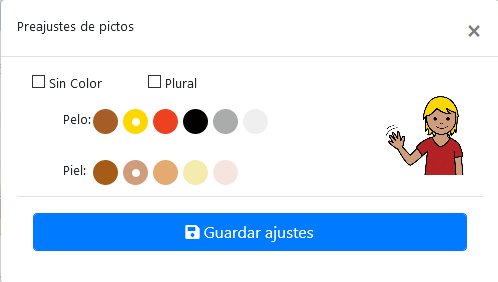
\includegraphics[width=0.7\linewidth]{Imagenes/Bitmap/modalPreajustePicto}
	\caption{Vista del modal del preajuste de pictos con las opciones color de pelo rubio y piel morena marcadas.}
	\label{fig:modalpreajustepicto}
\end{figure}



La interfaz del modal consiste en dos filas. La primera para los checkbox que marcan las opciones de plural y color, las cuales pueden estar activadas o desactivadas. La segunda fila es para elegir una de entre las distintas opciones de color disponibles tanto para el tono de piel como para el color de pelo. Está dispuesto de esa manera ya que si se marca algún checkbox, los botones radiales desaparecen. Esto se debe a que no es posible tener por ejemplo, un pictograma sin color y color de pelo rubio, previniendo así combinaciones que no estén disponibles.

A la izquierda cuenta con una previsualización para que el usuario conozca cómo afectan los atributos seleccionados al pictograma. Una vez el usuario esté conforme con los cambios, se envían al componente búsqueda de pictogramas las opciones seleccionadas.

Respecto a la construcción de las URLs se realiza de la siguiente manera:

\begin{enumerate}
	\item Se parte de la URL \texttt{https://static.arasaac.org/pictograms/id/id + \{options\} + \_500.png}. En la variable \texttt{options} se añadirán las opciones que modifiquen al pictograma.
	
	
	\item Dichas opciones deben estar  en un orden concreto utilizando los valores obtenidos del preajuste y el pictograma a crear. Por ejemplo, si se va a crear la URL del  pictograma “avión”, los ajustes relacionados con el color de pelo o piel no se aplicarían, ya que el picto no lo permite.
	 
	\item Un resultado posible para \texttt{option} sería: \texttt{\_action-future\_hair-020100 \_skin-A65C17}. El significado de cada etiqueta: \\ \texttt{\_action-future} añade la flecha en la esquina superior derecha indicando futuro y \texttt{hair}, y \texttt{skin} van asociados a su color hexadecimal correspondiente obtenido del preajuste. Si la etiqueta de \texttt{hair} fuera antes que la de \texttt{skin}, la URL creada no funciona. De ahí la importancia del orden.
	
	\item La URL creada se usa en cada pictograma mostrado en función de los preajustes, tal y como se puede observar en la Figura \ref{fig:buscarpictopreajuste}.
	
\end{enumerate}



% TODO: \usepackage{graphicx} required
\begin{figure}[h!]
	\centering
	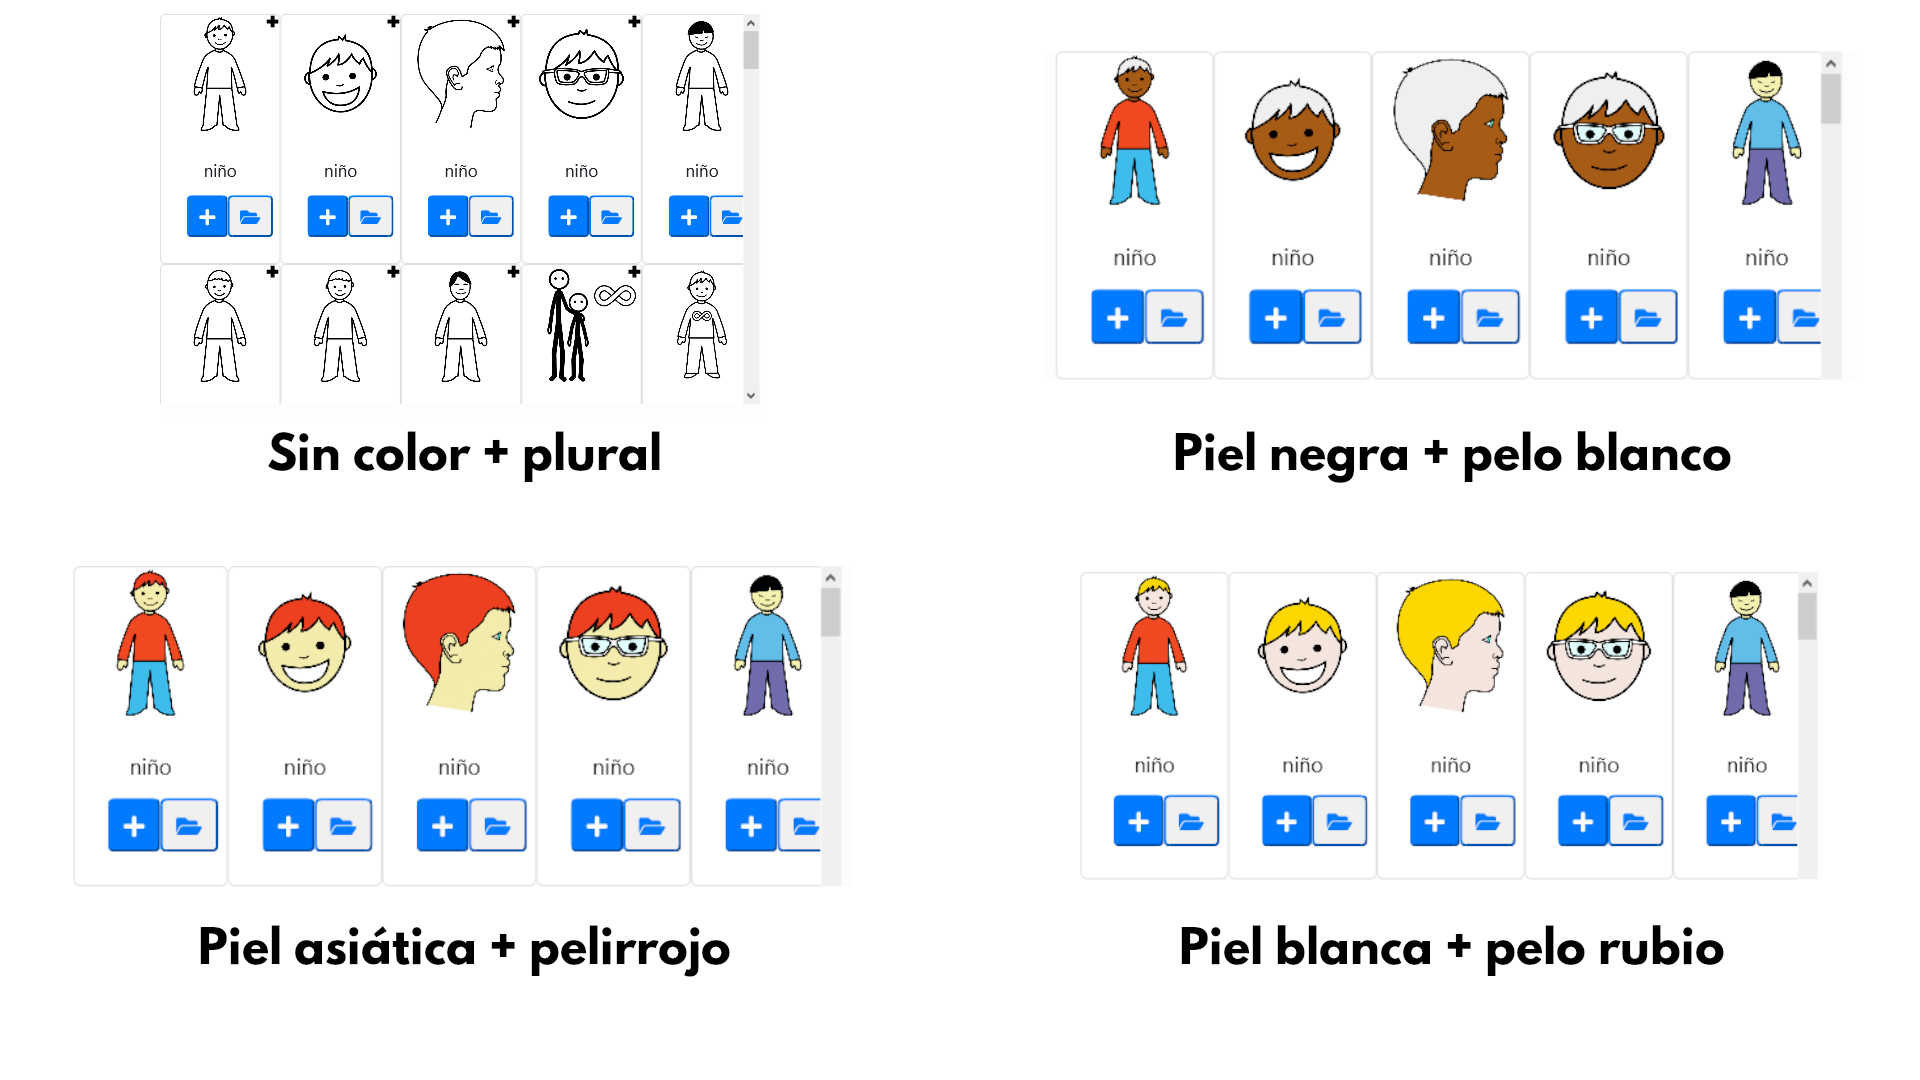
\includegraphics[width=0.9\linewidth]{Imagenes/Bitmap/buscarPictoPreajuste}
	\caption{Ejemplos de tipos de distintas combinaciones de preajuste}
	\label{fig:buscarpictopreajuste}
\end{figure}



\subsection{Historial de pictos}

Al añadir un pictograma al tablero, dicho pictograma se guarda en el historial que se mantiene entre sesiones. Para ello se ha utilizado LocalStorage\footnote{\url{https://developer.mozilla.org/en-US/docs/Web/API/Window/localStorage}}, el cual almacena una lista en la variable “recentPictos”. Dicha lista está compuesta por el objeto devuelto por la API de ARASAAC parseado a \texttt{string}, ya que los valores almacenados en LocalStorage solo pueden estar en formato \texttt{UTF-16 DOMString} que utiliza dos bytes por carácter.

Al pulsar sobre el botón de historial se cargarán y mostrarán todos los pictogramas encontrados en \texttt{recentPictos}. En caso que el historial esté vacío, se mostrará un mensaje indicándolo. Al igual que en el caso de la búsqueda, los pictogramas del historial se podrán añadir al tablero o a una lista, y son susceptibles del preajuste de pictogramas.

Es importante destacar que al realizar las pruebas se puso un límite a los pictogramas que se pudieran guardar en el historial. A partir de 300 aparecían pérdidas de rendimiento llegando a detener momentáneamente la página, motivo por el cual se redujo a 50.

\subsection{PictoItem}

PictoItem es el componente asignado para representar un pictograma en la cuadrícula. En la Figura \ref{fig:pictoitemmodificado} se puede ver su representación en el tablero: la mayor parte del componente lo abarca el pictograma, y debajo está su nombre. Las funcionalidades que tiene este PictoItem son la de editar el picto mediante el botón del lápiz y la de reproducir el sonido de su texto asociado mediante el botón \textit{play}. Respecto a su estructura interna, en su \texttt{state} almacena el objeto picto obtenido anteriormente de la API de ARASAAC, el preajuste asignado y \textit{flags} que indican si su modal de edición de  picto es visible o no. 


% TODO: \usepackage{graphicx} required
\begin{figure}[h!]
	\centering
	\includegraphics[width=0.4\linewidth]{Imagenes/Bitmap/pictoItemModificado}
	\caption{Vista de un PictoItem en la cuadrícula con preajuste de pelo y piel. }
	\label{fig:pictoitemmodificado}
\end{figure}


A continuación se detallarán las funcionalidades que ofrece  PictoItem.


\subsubsection{Editar Picto}

Tiene un funcionamiento igual al de preajuste de picto aunque se han añadido dos opciones más. Tal y como se puede ver en la Figura \ref{fig:modaleditarpicto}, éstas son el selector de tiempo verbal y  borde. El motivo de aparición de estas dos opciones en este modal y no en el preajuste es la de no abrumar al usuario. El Borde puede ser de utilidad para los usuarios que quieran resaltar el tipo de pictograma mediante un color. El selector de tiempo verbal sirve para indicar si una acción toma lugar en presente, pasado o futuro.

% TODO: \usepackage{graphicx} required
\begin{figure}[h!]
	\centering
	\includegraphics[width=0.7\linewidth]{Imagenes/Bitmap/modalEditarPicto}
	\caption{Vista de la interfaz del modal que muestra una edición de pictogramas con más opciones. En este caso, se ha seleccionado el tiempo futuro y el borde verde. }
	\label{fig:modaleditarpicto}
\end{figure}


\subsubsection{Reproducir sonido}


La función del botón es la de reproducir mediante audio el nombre del pictograma. Como se ha visto anteriormente, los pictogramas devueltos por la API pueden contar con locución si se consulta el parámetro “\textit{hasLocution}”. En caso de contar con locución, se accede a la URL\footnote{\url{https://privateapi.arasaac.org/api/locutions/es/}} que contiene la pista de voz asociada y se reproduce. 
En caso de no contar con locución se ha usado \textit{SpeechSynthesisUtterance}\footnote{\url{https://developer.mozilla.org/en-US/docs/Web/API/SpeechSynthesisUtterance}} para que haga una función similar en el resto de pictogramas. Está configurada para que sintetize la voz en español y es compatible con todos los navegadores modernos.

\subsection{Reglas de diseño de usabilidad}
 Las reglas de diseño utilizadas en esta funcionalidad han sido:

\begin{itemize}
	\item \textbf{Coherencia}: esta herramienta hace usos de iconos para ayudar al usuario de una manera visual a saber que acción va a realizar. Los iconos utilizados son: una lupa para realizar la búsqueda, un icono al lado de la lupa para ver el historial de búsqueda y unos engranajes en la parte de la derecha para realizar el preajuste de los pictogramas.
	
	También se utilizan los iconos de “+” para añadir el pictograma al tablero y el icono de la carpeta para añadir el pictograma a una nueva lista o a una ya creada.
	
	En PictoItem también se utilizan iconos que representarán distintas funcionalidades sobre el pictograma. Por ejemplo, en la esquina superior derecha hay una “x” para eliminar el pictograma y en la parte inferior iconos de un lápiz para editar el pictograma y un icono de un triángulo para reproducir la palabra. Algunos iconos como la “x” o el icono del lápiz también será utilizados por otros ítems y estarán en las mismas posiciones y harán funciones similares. Esto se hace para crear uniformidad y ayudar al usuario a familiarizarse con la aplicación.
	
	
	\item \textbf{Usabilidad universal}: el principio de usabilidad reconoce las necesidades de los distintos tipos de usuarios ya sean nuevos o expertos en la aplicación. Esto queda reflejado en el apartado de búsqueda de pictogramas con la opción de preajuste de pictogramas. Por ejemplo, un usuario en la aplicación añadiría un pictograma al tablero y después lo editaría, pero mediante el preajuste permite añadir varios pictogramas sin tener que editarlos individualmente.
	
	\item \textbf{Retroalimentación informativa}: el usuario, tras realizar la búsqueda, verá visualmente todos los pictogramas cuyo significado coincide con la palabra a buscar. También tras pulsar el botón “+” sobre un pictograma, este automáticamente se añadirá al tablero.
	
	
	\item \textbf{Permitir deshacer acciones de forma fácil}: en caso de escribir mal la palabra al realizar la búsqueda el usuario podrá borrarla y volver a escribirla correctamente para buscar los pictogramas que correspondan con esa palabra.
\end{itemize}


\section{Traducir frase a pictogramas}
\label{cap5:sec:traduccion}
La herramienta de traducción de frase a pictograma se encuentra en la segunda pestaña que agrupa las herramientas para añadir pictogramas e imágenes, tal y como se puede ver en la Figura \ref{fig:traducirfraseinicial}. Cuenta con un ítem propio llamado FraseItem, que agrupa los pictogramas de la traducción para ser desplazados en bloque por la cuadrícula.

La traducción de frase a pictogramas, como su nombre indica, ofrece una interfaz que permite al usuario escribir una frase y recibir la traducción en pictogramas. Nuevamente, en la Figura \ref{fig:traducirfraseinicial} se puede ver la interfaz inicial de la traducción a frase, muy similar a la vista en la búsqueda de picto en la Figura \ref{fig:buscarpicto2}. 

% TODO: \usepackage{graphicx} required
\begin{figure}[h!]
	\centering
	\includegraphics[width=0.7\linewidth]{Imagenes/Bitmap/traducirFraseInicial}
	\caption{Interfaz inicial Traducción frase a pictograma.}
	\label{fig:traducirfraseinicial}
\end{figure}

 
La traducción es realizada mediante la API de ARASAAC. Aunque no cuenta con una traducción dedicada a frases, se traduce el texto palabra a palabra de la frase escrita. Por cada palabra se realizará una búsqueda que devolverá entre 0 o más pictogramas. Inicialmente la traducción se iba a realizar mediante la API de accesibilidad del grupo NIL, que cuenta con una función dedicada a la traducción de frases a pictogramas. En la Sección \ref{cap5:sec:nilgroup} se explicará por qué no ha sido utilizada. 


El resultado de la traducción no está fijado a un pictograma concreto por palabra, sino que puede haber varios. Es por ello que se devuelven de un modo u otro varios pictogramas posibles por cada palabra de la frase.  En la Figura \ref{fig:traduccionpicto} se puede ver cómo la interfaz permite navegar entre los pictogramas alternativos mediante dos botones.
Estos botones permiten avanzar y retroceder entre los pictogramas alternativos que se muestran por cada palabra. Por último destacar que el botón “Colocar al tablero” no se activa hasta que no hay una frase traducida, como se puede ver en las Figuras \ref{fig:traducirfraseinicial} y \ref{fig:traduccionpicto}. 

% TODO: \usepackage{graphicx} required
\begin{figure}[h!]
	\centering
	\includegraphics[width=0.7\linewidth]{Imagenes/Bitmap/traduccionPicto}
	\caption{Resultado de la traducción de una frase}
	\label{fig:traduccionpicto}
\end{figure}

El componente también permite añadir los pictogramas de manera individual al pulsar sobre el botón “+”, tal y como sucedía en búsqueda de pictograma. En caso de que se pulse sobre “Colocar al tablero”, se colocarán en el tablero todos los pictogramas juntos en un único elemento FraseItem. 

\subsection{FraseItem}

Como se puede ver en la Figura \ref{fig:fraseitemoriginal} este tipo de  ítem agrupa todos los pictogramas recibidos de la traducción. De esta manera el usuario, para desplazarlo por el tablero, no tiene que mover cada pictograma de manera individual. Este ítem cuenta además con la posibilidad de ocultar pictogramas ya que el usuario podría no querer que se muestre alguno. Para ello se ha de presionar en el botón de edición con el icono del lápiz. 

% TODO: \usepackage{graphicx} required
\begin{figure}[h!]
	\centering
	\includegraphics[width=0.7\linewidth]{Imagenes/Bitmap/fraseItemOriginal}
	\caption{Vista de FraseItem en la cuadrícula}
	\label{fig:fraseitemoriginal}
\end{figure}


Al ser presionado aparecerá un nuevo modal como se ve en la Figura \ref{fig:modaleditarfraseitem}. Está compuesto por una previsualización de la frase en la parte superior, y en la parte inferior los pictogramas que componen la frase junto al botón que permite esconderlos o mostrarlos. Dicho botón cambiará de apariencia según el estado de visualización del pictograma. Si es visible el botón representa un ojo en azul, y en caso contrario se representará mediante un ojo tachado en rojo ocultando el pictograma de la previsialización superior. Al presionar alguno de ellos, se actualiza la previsualización. Por último, debajo existe un campo de texto donde se puede editar el contenido de la frase.
En la Figura \ref{fig:fraseitemmidificada} se puede ver un ejemplo de cómo quedaría el ítem tras aplicar los cambios. 

% TODO: \usepackage{graphicx} required
\begin{figure}[h!]
	\centering
	\includegraphics[width=0.7\linewidth]{Imagenes/Bitmap/modalEditarFraseItem}
	\caption{Vista del modal de edición del FraseItem}
	\label{fig:modaleditarfraseitem}
\end{figure}

% TODO: \usepackage{graphicx} required
\begin{figure}[h!]
	\centering
	\includegraphics[width=0.7\linewidth]{Imagenes/Bitmap/fraseItemMidificada}
	\caption{FraseItem tras  aplicar los cambios}
	\label{fig:fraseitemmidificada}
\end{figure}

\subsection{Reglas de diseño de usabilidad}
\label{cap5:reglasBusqueda}
 Las reglas de diseño utilizadas en esta funcionalidad han sido:
 
\begin{itemize}
	\item \textbf{Coherencia}: al igual que en el buscador de pictogramas se utiliza el icono de la lupa para realizar la traducción de la frase. También se utilizan unas flechas como iconos para ver todos los pictogramas asociados a cada palabra, y al igual que en el buscador de pictogramas se incluye el icono “+” para añadir individualmente un pictograma.
	
	\item \textbf{Retroalimentación informativa}: tras pulsar el botón para realizar la traducción de la frase se le mostrará al usuario todos los pictogramas asociados a las palabras de la frase.  También si el usuario pulsa sobre las flechas de un pictograma se le mostrará otros pictogramas con un significado similar permitiendo así escoger el que más le guste al usuario. Por último, tras haber realizado una traducción de una frase y al pulsar sobre el botón para colocarla en el tablero, la frase se añadirá al tablero informando de esta manera que la acción se ha realizado correctamente.
	
	\item \textbf{Prevenir errores}: para evitar que el usuario añada una frase vacía al tablero, el botón de “Colocar al tablero” se habilitará cuando se haya realizado una traducción. Tras borrar la frase en el campo de texto el botón se volverá a deshabilitar.
	
	
	\item \textbf{Permitir deshacer acciones de forma fácil}: si el usuario escribe mal la frase a traducir siempre podrá corregir los errores de escritura y realizar la traducción de la frase. También podrá eliminar la fraseItem del tablero pulsando sobre el icono “+” de su interior.
	
\end{itemize}





\section{Añadir imagen al tablero}
\label{cap5:sec:imagen}
Añadir una imagen al tablero se encuentra en la tercera pestaña que agrupa todas las herramientas que añaden pictogramas o fotos a la cuadrícula. Como se puede ver en la Figura \ref{fig:cargarfotopestana}, su interfaz inicial consiste en un simple botón que carga una imagen del explorador de archivos del dispositivo. Está especificado que solo acepte archivos de tipo imagen, previniendo así posibles errores del usuario. 

% TODO: \usepackage{graphicx} required
\begin{figure}[h!]
	\centering
	\includegraphics[width=0.7\linewidth]{Imagenes/Bitmap/cargarFotoPestaña}
	\caption{Interfaz inicial al añadir una imagen al tablero}
	\label{fig:cargarfotopestana}
\end{figure}


Al cargar la imagen correctamente, tal y como se puede ver en la Figura \ref{fig:addphotoitem}, se mostrará: 

\begin{itemize}
	\item Una previsualización de la imagen.
	\item Un campo de texto para añadirlo debajo de la imagen.
	\item Un botón para añadir la imagen a la cuadrícula.
\end{itemize}

% TODO: \usepackage{graphicx} required
\begin{figure}[h!]
	\centering
	\includegraphics[width=0.7\linewidth]{Imagenes/Bitmap/addPhotoItem}
	\caption{ Vista de la Interfaz al cargar una imagen}
	\label{fig:addphotoitem}
\end{figure}



Al presionar el botón de añadir, antes de enviar la información de la foto, se obtiene su valor de alto y ancho en píxeles. Estos datos serán utilizados para conocer la proporción de la imagen. Respecto al acceso a los datos de la foto, se realiza por una URL que funciona únicamente en la sesión vigente generada mediante \texttt{URL.createObjectURL}\footnote{\url{https://developer.mozilla.org/en-US/docs/Web/API/URL/createObjectURL}}.

Al enviar la información de la foto a la capa superior se envían los siguientes parámetros: 

\begin{itemize}
	\item URL de la imagen.
	\item Ancho y alto en píxeles.
	\item Texto inferior. En caso de no haber sido escrito nada, se enviará vacío.
\end{itemize}

Se estudiaron otras maneras de cargar las imágenes, como importarlas desde Google Drive o un archivo zip. Sin embargo fueron descartadas. En la Sección \ref{cap5:addImageCut} se especificarán los motivos. 

\subsection{PhotoItem}

Su representación en el tablero es la imagen dentro del ítem. El ancho y alto del ítem es proporcional a la imagen original, como se calculó anteriormente. 

Respecto al texto inferior, se puede ver en la Figura \ref{fig:photoitemtexto} que puede aparecer o no. Si se ha recibido un texto inferior, éste aparecerá en un espacio reservado para él debajo de la imagen. En caso contrario la imagen abarcará la totalidad del ítem.

% TODO: \usepackage{graphicx} required
\begin{figure}[h!]
	\centering
	\includegraphics[width=0.7\linewidth]{Imagenes/Bitmap/photoItemTexto}
	\caption{Ejemplod de PhotoItem con y sin texto}
	\label{fig:photoitemtexto}
\end{figure}


En la Figura \ref{fig:photoitemerror} se ejemplifica qué pasaría si en vez de calcular la proporción de la imagen, se dejara siempre con un ancho y alto fijo apareciendo espacios en blanco.

% TODO: \usepackage{graphicx} required
\begin{figure}[h!]
	\centering
	\includegraphics[width=0.7\linewidth]{Imagenes/Bitmap/photoItemError}
	\caption{Ejemplo de PhotoItemn si no se mantuviera la proporción según el tamaño de la imagen}
	\label{fig:photoitemerror}
\end{figure}

\subsection{Reglas de diseño de usabilidad}

 Las reglas de diseño utilizadas en esta funcionalidad han sido:
\begin{itemize}
	\item \textbf{Coherencia}: como en las otras herramientas, se hace uso de iconos para proporcionar al usuario una manera más simple y visual de la acción va a realizar. Un ejemplo de icono utilizado es el botón con el “+” para añadir la imagen al tablero. Al igual que en otros items como PictoItem o FraseItem el componente PhotoItem también tiene un icono “x” para poder ser eliminado del tablero.
	
	\item \textbf{Retroalimentación informativa}: tras pulsar sobre el botón “Cargar foto” y seleccionar una imagen, se mostrará en la parte de abajo una previsualización de la imagen. Esto permite al usuario ver si la imagen seleccionada es la correcta.
	También podemos ver que esta regla se cumple al pulsar sobre el botón con el icono “+”, el cual añadirá al tablero la imagen seleccionada.
	
	
	\item \textbf{Permitir deshacer acciones de forma fácil}:  tras cargar una imagen y no ser la deseada por el usuario, este podrá volver a seleccionar una nueva imagen que posteriormente se previsualizará. También se podrá eliminar un PhotoItem que ya esté añadido en el tablero pulsado sobre el icono “+” de su interior.
	
\end{itemize}



\section{Listas de pictogramas}
\label{listapictos}

Esta herramienta permite crear distintas listas donde el usuario podrá añadir los pictogramas que desee.
Para implementar esta herramienta se necesita tener una estructura donde se guarde el nombre de cada una de las listas y todos los elementos PictoItem que contenga. 

\subsection{Añadir y crear a una lista}

Para crear una lista o añadir un pictograma a una lista existente, el usuario deberá pulsar sobre el icono de la carpeta de un pictograma tras realizar una búsqueda, tal y como se puede ver en la Figura \ref{fig:buscarpicto2}. Tras pulsar el icono se desplegará un modal donde dependiendo del estado de las listas mostrará un menú u otro. En el caso de que no haya ninguna lista simplemente se mostrará la opción de crear una lista donde se deberá introducir el nombre de la lista a crear, mientras que si ya había alguna lista creada se mostrará un menú con la posibilidad de añadir el pictograma seleccionado a una lista existente o crear una nueva lista. Un ejemplo de esto lo podemos ver en la Figura \ref{fig:modalescoleccion} donde el modal de la izquierda aparece cuando no existe ninguna lista y el de la derecha cuando ya existe al menos una lista. Además la lista mostrada en el modal de la izquierda será la última lista modificada.


% TODO: \usepackage{graphicx} required
\begin{figure}[h!]
	\centering
	\includegraphics[width=0.7\linewidth]{Imagenes/Bitmap/modalesColeccion}
	\caption{Vistas del modal con ninguna lista y al menos una, respectivamente}
	\label{fig:modalescoleccion}
\end{figure}


Para informar al usuario de las acciones, tanto la de crear una nueva lista, como añadir un pictograma a una lista existente se han utilizado alertas (mensajes). Estas alertas a parte de dar una cierta información al usuario también sirven para tener un cierto control de errores para que el usuario no cree dos listas con el mismo nombre o que no añada un pictograma dos veces a una lista.


\begin{itemize}
	\item En el caso de que se haya podido realizar la acción con éxito se mostrará un pequeño mensaje descriptivo de la acción en verde (Figura \ref{fig:alertlistapicto}).
	
	% TODO: \usepackage{graphicx} required
	\begin{figure}[h!]
		\centering
		\includegraphics[width=0.7\linewidth]{Imagenes/Bitmap/alertListaPicto}
		\caption{ Alerta tras añadir satisfactoriamente un pictograma a la lista}
		\label{fig:alertlistapicto}
	\end{figure}
	
	
	\item  En el caso de que la acción no se haya podido realizar correctamente se informará al usuario con un mensaje en rojo, como el que se ve en la Figura \ref{fig:alerterrorlistapicto}, informando al usuario el por qué no ha podido realizarla.
	
	% TODO: \usepackage{graphicx} required
	\begin{figure}[h!]
		\centering
		\includegraphics[width=0.7\linewidth]{Imagenes/Bitmap/alertErrorListaPicto}
		\caption{Alerta de acción no permitida}
		\label{fig:alerterrorlistapicto}
	\end{figure}
	
	
	
\end{itemize}

\subsection{Gestión de listas de pictogramas}

Otras funcionalidades que podemos encontrar en esta herramienta es la posibilidad de importar y exportar las listas creadas.
Para la funcionalidad de exportar guardaremos el estado actual de las listas en un fichero con extensión “.json”. Para la generación de este documento se utilizará la función \textit{JSON.stringify()}, la cual nos permitirá crear la estructura propia de los json y posteriormente generar el documento con ese contenido.

La funcionalidad de importar cargará el estado de las listas a partir del archivo creado anteriormente. Para ello se hará uso de la función \textit{JSON.parse()}, la cual convertirá el json a la estructura de listas requerida. En caso de ya existir listas en la aplicación, las nuevas listas cargadas se añadirán a las ya existentes. 

Por último, las listas existentes se encuentran en el apartado “Mis listas de pictogramas”, como se muestra en la Figura \ref{fig:lisapictosel}. Para visualizar una de ellas deberemos seleccionar el nombre de esta de entre todas las disponibles. A continuación, al igual que en el apartado de búsqueda de pictograma, se mostrarán todos los pictogramas con su imagen, texto correspondiente y el botón de “+” que permite añadirlo a la cuadrícula como un PictoItem visto anteriormente.

% TODO: \usepackage{graphicx} required
\begin{figure}[h!]
	\centering
	\includegraphics[width=0.7\linewidth]{Imagenes/Bitmap/lisaPictoSel}
	\caption{Vista de las listas de pictogramas}
	\label{fig:lisapictosel}
\end{figure}

\subsection{Reglas de diseño de usabilidad}

Las reglas de diseño utilizadas en esta funcionalidad han sido:
\begin{itemize}
	\item \textbf{Coherencia}: se ha utilizado el icono de una carpeta para todas las acciones que tiene que ver con las listas de pictogramas. Este icono aparece tanto en los pictogramas devueltos tras realizar una búsqueda simple como en el apartado “Mis listas de pictogramas”.  También se utilizan iconos similares en los botones de los modales, como por ejemplo en el botón para añadir una nueva lista cuyo icono es una carpeta con un más dentro, o en el apartado añadir a una lista existente donde el icono es una flecha señalando a un documento, haciendo alusión a que se va a incluir en la lista indicada previamente.
	
	\item \textbf{Retroalimentación informativa}: para informar al usuario de si una acción se ha podido realizar correctamente o no se han utilizado las alertas. Las alertas utilizadas pueden ser de dos tipos: verdes para las acciones realizadas correctamente y las rojas para las acciones que han dado algún tipo de error como crear dos listas con el mismo nombre. Éstas aparecen siempre en la parte superior de la pantalla junto con un texto descriptivo de la acción que se ha realizado para asegurar que sean vistas con facilidad.
	
	\item \textbf{Prevenir errores}: la aplicación está diseñada para prevenir que el usuario cometa un error y en caso de error sea detectado e informe con un breve mensaje describiéndolo. Este tipo de patrón se aplica en todas las acciones correspondientes a las listas de pictogramas a la hora de crear una lista, donde se comprueba que la lista tenga un nombre y no se repita con otra existente, y al añadir un pictograma a una lista donde se verifica que no se haya añadido anteriormente. En caso de error se utilizarán las alertas con un mensaje informando del problema.
	
	
	\item \textbf{Permitir deshacer acciones de forma fácil}: en caso de que el usuario cree una lista por error la podrá borrar desde el apartado “Mis listas de pictogramas” donde deberá seleccionar la lista creada y pulsar sobre el botón de borrar lista.
	
\end{itemize}


\section{Texto}

Esta herramienta permite añadir un cuadro de texto a la cuadrícula. Como opciones de personalización de texto se ofrece la posibilidad al usuario de seleccionar una tipografía entre las seis posibles. Las tipografías elegidas son las más utilizadas dentro del ámbito educativo.

Esta herramienta se puede encontrar en el apartado de “Personalización de tablero”, donde se podrán seleccionar distintas tipografías y escribir el texto que se va a añadir a la cuadrícula.

Como se puede ver en la Figura \ref{fig:anadirtexto} en la parte superior se puede elegir una tipografía y a su derecha ver una previsualización de ésta. Debajo, está el campo de texto donde se escribirá la frase seguido del botón para añadirla a la cuadrícula.

% TODO: \usepackage{graphicx} required
\begin{figure}[h!]
	\centering
	\includegraphics[width=0.7\linewidth]{Imagenes/Bitmap/añadirTexto}
	\caption{Vista de la selección de fuente y campo de texto}
	\label{fig:anadirtexto}
\end{figure}


Para poder implementar este componente, en su estructura se guardará el texto que se vaya a añadir a la cuadrícula y la tipografía seleccionada.

A diferencia de otros elementos como los pictogramas en los que el ancho y alto del ítem era proporcional, en el texto se permite ajustar ambas propiedades de manera independiente.

\subsection{TextoItem}
\label{cap5:sec:texto}
Al añadir el texto a la cuadrícula, el ancho del ítem se ajustará al número de caracteres del texto. En la parte inferior del ítem como se ve en la Figura \ref{fig:fraseitem1} se encuentran tres botones, dos para reducir y aumentar el tamaño de la fuente del texto y otro para editar su contenido.

% TODO: \usepackage{graphicx} required
\begin{figure}[h!]
	\centering
	\includegraphics[width=0.7\linewidth]{Imagenes/Bitmap/fraseItem1}
	\caption{Representación del TextoItem en la cuadrícula}
	\label{fig:fraseitem1}
\end{figure}


Al pulsar sobre el icono del lápiz se desplegará el modal de edición de ítem. Como se ve en la Figura \ref{fig:modaleditartexto} cuenta con un campo donde se puede ver y editar el contenido actual del texto. Esto resultará muy útil para corregir errores ortográficos. Tras pulsar sobre el botón “Cambiar texto”, el ancho del ítem se ajustará de nuevo en función del nuevo número de caracteres.

% TODO: \usepackage{graphicx} required
\begin{figure}[h!]
	\centering
	\includegraphics[width=0.7\linewidth]{Imagenes/Bitmap/modalEditarTexto}
	\caption{Vista del modal para editar un TextoItem}
	\label{fig:modaleditartexto}
\end{figure}

\subsection{Reglas de diseño de usabilidad}

 Las reglas de diseño utilizadas en esta funcionalidad han sido:
\begin{itemize}
	\item \textbf{Coherencia}:  un TextoItem añadido al tablero contará con múltiples botones, en la parte superior derecha tendrá una “x” para eliminar el texto del tablero y en la parte inferior dos iconos de unas lupas para ampliar o reducir la fuente del texto y un icono de un lápiz para poder editar el contenido.
	
	\item \textbf{Retroalimentación informativa}: en el apartado de “Personalización del tablero” el usuario podrá seleccionar distintos tipos de fuentes de letras donde verá al instante un ejemplo de la fuente seleccionada. Además, cuando el usuario pulse sobre el botón de “+Texto” verá de manera instantánea el texto en el tablero de la aplicación. De esta manera se le informa al usuario de que la acción se ha realizado correctamente. También afecta a la acción de borrar el texto del tablero, ya que cuando el usuario pulse sobre el icono “x” automáticamente se borrará del tablero.
	
	
	\item \textbf{Permitir deshacer acciones de forma fácil}: en caso de haber añadido el texto al tablero con una falta de ortografía el usuario podrá editar el contenido del TextoItem pulsando sobre el icono del lápiz. También podrá eliminar el texto del tablero en caso de que haya sido añadido por error, para esto deberá pulsar sobre el icono “x” situado en la esquina superior derecha.
	
\end{itemize}



\section{Iconos}
\label{cap5:sec:iconos}
El componente icono permite añadir a la cuadrícula iconos y personalizarlos. Los iconos disponibles son: cuadrado, tick, barra y corazón, como se muestra en la Figura \ref{fig:herramientaitems}. El componente está formada por una estructura donde se guarda el tipo de icono, el color y la opacidad.

% TODO: \usepackage{graphicx} required
\begin{figure}[h!]
	\centering
	\includegraphics[width=0.7\linewidth]{Imagenes/Bitmap/herramientaItems}
	\caption{Vista de los botones que añaden iconos}
	\label{fig:herramientaitems}
\end{figure}


A la hora de mostrar los iconos en la cuadrícula hay que hacer una distinción entre el cuadrado y el resto de los iconos ya que la forma en la que se muestran es distinta.

Para generar un cuadrado se hace uso de las formas geométricas básicas que ya están implementadas en SVG. Este lenguaje de marcas permite crear figuras geométricas y personalizar su aspecto. Para representar el cuadrado se ha de incluir la etiqueta \textit{<rect/>} (etiqueta para generar un cuadrado) y añadir las propiedades que queremos que tenga como por ejemplo altura, ancho, grosor de los bordes del cuadrado, color u opacidad.

Sin embargo, para el resto de los iconos se utilizan recursos obtenidos de FontAwesome\footnote{\url{https://fontawesome.com/}}. Este framework tiene implementado iconos vectoriales que al igual que con el cuadrado, permiten la personalización de los iconos respecto a el color, tamaño y opacidad. Para mostrarlos se deberá incluir la clase correspondiente de cada icono especificada en el apartado tipo de la estructura.

En la Figura \ref{fig:ejemplopictoitem} se puede ver que estos iconos se pueden superponer a los pictogramas para realzar ideas.

% TODO: \usepackage{graphicx} required
\begin{figure}[h!]
	\centering
	\includegraphics[width=0.7\linewidth]{Imagenes/Bitmap/ejemploPictoItem}
	\caption{Ejemplo de uso de iconos sobre algunos pictogramas}
	\label{fig:ejemplopictoitem}
\end{figure}

 
Aunque la forma de visualizarlos se hace de manera distinta dependiendo del icono, todos ellos permiten editar ciertos aspectos. Es por ello por lo que se incluyó la funcionalidad de editar. Para poder editar un icono añadido a la cuadrícula tendremos que pulsar sobre el icono del lápiz, al pulsarlo aparecerá un modal, como el de la Figura \ref{fig:modalpictoitem} donde se podrá modificar el color y la opacidad del icono.  

% TODO: \usepackage{graphicx} required
\begin{figure}[h!]
	\centering
	\includegraphics[width=0.7\linewidth]{Imagenes/Bitmap/modalPictoItem}
	\caption{Vista del modal de edición de iconos.}
	\label{fig:modalpictoitem}
\end{figure}

\subsection{IconoItem}

Cuando un icono se añade al tablero de la aplicación este tendrá una opacidad y color por defecto. A los iconos corazón y barra tendrá por defecto el color rojo y una opacidad al 50\%, y el icono del tick tiene como color por defecto será el verde y una opacidad del 50\%. El hecho de que los iconos tengan por defecto esa opacidad es debido a que están planteados para estar superpuestos encima de los pictogramas, por lo que han de ser translúcidos para ver el pictograma que se encuentra debajo del icono. Por último, el icono del cuadrado por defecto será negro y la opacidad del 100\% ya que están planteados para ser opacos.

En el IconoItem se incluyen dos botones, una “x” en la esquina superior derecha que sirve para eliminar el icono del tablero y un icono de un lápiz en la parte inferior que permite editar el icono. Para poder editar un icono añadido a la cuadrícula tendremos que pulsar sobre el icono del lápiz, al pulsarlo aparecerá un modal, como el de la Figura \ref{fig:modalpictoitem} donde se podrá modificar el color y la opacidad del icono.

\subsection{Reglas de diseño de usabilidad}
 Las reglas de diseño utilizadas en esta funcionalidad han sido:
\begin{itemize}
	\item \textbf{Coherencia}: en el apartado “Personalización del tablero” se muestran todos los iconos disponibles que se pueden añadir al tablero, permitiendo de esta manera mostrar al usuario como son esos iconos antes de ser añadidos. El IconoItem cuenta con un botón en la esquina superior derecha para eliminarlo y un botón con el icono de un lápiz para poder editarlo, al igual que otros items.
	
	
	\item \textbf{Retroalimentación informativa}: al pulsar sobre uno de los botones con iconos en el apartado “Personalización del tablero” automáticamente se añadirá al tablero. De esta manera se informa al usuario de que la acción para añadir un icono se ha realizado correctamente. Para la acción contraria de eliminar un IconoItem simplemente se eliminará del tablero dando a entender al usuario que el icono se ha podido eliminar correctamente. Otra acción que se ve reflejada en esta regla es que tras editar un icono y cerrar el modal, se le asignará al icono el nuevo color y opacidad visualizando el nuevo resultado al instante.
	
	
	\item \textbf{Permitir deshacer acciones de forma fácil}: en caso de añadir un icono por error el usuario podrá eliminarlo desde el tablero. También se permite al usuario volver a cambiar el color o la opacidad de un icono las veces que desee.
	
\end{itemize}


\section{Descargar Tablero}
\label{cap5:descargar}

Esta herramienta permite descargar la cuadrícula como imagen. Para ello se utiliza la librería html2tocanvas\footnote{\url{https://html2canvas.hertzen.com/}}. Ésta librería además permite seleccionar la calidad de descarga de la imagen. Por ello que se ha creado un modal como se puede ver en la Figura \ref{fig:modaldescargartablero} donde el usuario puede elegir la calidad deseada, siendo la calidad alta la elegida por defecto. 

Inicialmente se planteó la posibilidad de descargar estos tableros como PDF pero esta opción no se implementó por falta de tiempo.

% TODO: \usepackage{graphicx} required
\begin{figure}[h!]
	\centering
	\includegraphics[width=0.7\linewidth]{Imagenes/Bitmap/modalDescargarTablero}
	\caption{Vista del modal para descargar tablero}
	\label{fig:modaldescargartablero}
\end{figure}



\section{Funcionalidades no implementadas}
\label{cap5:noimplementadas}

Durante el desarrollo de PictUp! se abandonaron algunas funcionalidades debido principalmente a la falta de tiempo o problemas con su integración en la aplicación. A continuación se detallarán los problemas surgidos por cada funcionalidad. 


\subsection{Traducción de frase}
Se trata de la funcionalidad más problemática pues se invirtieron varias semanas en solventarla sin éxito. Una prioridad era la utilización de la NIL-WS-API, pues ofrece una traducciones muy acertadas. A continuación se explicarán los distintos problemas que surgieron durante su implementación.  

\label{cap5:sec:nilgroup}

NIL Web Service\footnote{\url{https://holstein.fdi.ucm.es/nil-ws-api/}} es una API que devuelve información relativa a palabras y textos orientada a resolver problemas de accesibilidad a través del lenguaje. Respecto al tratamiento de palabras, permite buscar sinónimos, antónimos, emociones de las palabras, etc. Para el tratamiento de textos, permite  traducir un texto a pictogramas, listar las emociones de un texto o resumir, entre otras funcionalidades. 

Originalmente la traducción de pictogramas en esta aplicación fue creada específicamente para trabajar con esta API. No obstante también ha causado varios inconvenientes, relativos a los pictogramas que usa la API y los errores causados por CORS. 

La API cuenta con una base de datos propia con una gran cantidad de pictogramas. Pero al traducir un texto a pictogramas, esta devuelve por cada palabra o lema, una lista de identificadores. En su mayoría dichos identificadores coinciden con los de los pictogramas de ARASAAC, pero existen otros que no. Estos pictogramas que no comparten identificador con los de ARASAAC suponen un problema, ya que no se puede obtener toda la información deseada, como por ejemplo el texto, audio y modificaciones. Es por ello que PictoItem se modificó para incluir estos pictogramas suprimiendo la posibilidad de personalizar o reproducir el audio. A continuación se especificará sobre el funcionamiento y problemática asociada a CORS.


Cross Origin Resource Sharing\footnote{\url{https://developer.mozilla.org/en-US/docs/Web/HTTP/CORS}}, es un mecanismo de cabeceras http que permite a un servidor dar permiso a otros dominios para cargar recursos del mismo. Por razones de seguridad los navegadores restringen las peticiones de dominio cruzado desde los scripts del navegador. 


Como el servicio de traducción de NIL-WS-API sigue operativo pero descontinuado, no cuenta con la configuración CORS y por tanto no puede recibir peticiones POST de otras webs. Después de comprender el problema se estudió que la solución es crear un backend para PictUp!. Dicho backend está creado exclusivamente para resolver esta petición. El componente de traducción envía la petición al backend, el cual la resolverá gestionando los CORS. En la próxima Sección \ref{backend} se explicará cómo fue creado. 

Después de crear y configurar el backend de manera local, y ver que el componente funcionaba sin complicaciones, apareció otro error con la biblioteca html2canvas\footnote{\url{https://html2canvas.hertzen.com/}}, encargada de crear una imagen a partir de la cuadrícula y sus ítems. Esto es debido a que las imágenes que retorna NIL-WS-API son un recurso externo y la biblioteca htm2canvas desconoce su fuente. Por ello al descargar la imagen del tablero estos pictogramas no aparecían representados dejando un hueco en blanco.


\subsection{Backend}
\label{backend}

El backend fue creado mediante Express\footnote{\url{http://expressjs.com/en/starter/installing.html}}. Se trata de un framework de Node.js que permite gestionar llamadas a API de manera sencilla. Express cuenta con una dependencia que gestiona los CORS\footnote{\url{https://www.npmjs.com/package/cors }}, la cual fue usada para realizar el método post a la API de NIL. 

Para esquematizar cómo se obtienen los pictogramas de la API de NIL, se puede ver en la Figura \ref{fig:diagramaconexiones} un diagrama de las llamadas que se realizan entre las aplicaciones. 

% TODO: \usepackage{graphicx} required
\begin{figure}[h!]
	\centering
	\includegraphics[width=0.7\linewidth]{Imagenes/Bitmap/diagramaConexiones}
	\caption{Diagrama de conexiones entre aplicaciones para traducir una frase}
	\label{fig:diagramaconexiones}
\end{figure}


Después de varias semanas investigando todos estos problemas, finalmente se detuvo el desarrollo de este componente ya que la fecha para mostrar la web a los usuarios se acercaba. Al tener un prototipo funcional de traducción mediante la API de ARASAAC, aunque asumiendo la baja calidad sintáctica de ésta se consideró suficiente para estudiar la facilidad de uso de la interfaz por parte de los usuarios.




\subsection{Añadir imagen}
\label{cap5:addImageCut}

Originalmente hubo dos aproximaciones sobre la inserción de imágenes. La primera consistía en poder cargar un archivo comprimido zip mediante la librería JSZip\footnote{\url{https://stuk.github.io/jszip/}} que contaba con funciones para descomprimir archivos. El objetivo era automatizar la colocación de imágenes sobre el tablero, mediante un zip que almacenara éstas junto a un documento con la información de cada una. Dicho documento incluiría el nombre, la posición y el tamaño de cada imagen colocada en la cuadrícula. Descomprimiendo dicho zip, las imágenes volverían a ser colocadas a la posición original.

La otra aproximación ofrecía la posibilidad de conectarse mediante la API de Google Drive\footnote{\url{https://developers.google.com/drive/api/v3/about-sdk }} para que el usuario pudiese acceder a sus fotos almacenadas en su cuenta. 

Pese a haber dedicado varias semanas a cada una de estas opciones en proyectos independientes, fueron abandonadas por no obtener resultados satisfactorios. En el caso de JSZip, aunque la compresión de las fotos y descarga del zip funcionara correctamente, surgieron problemas con la librería a la hora de descomprimir los archivos. Respecto a la API de Google Drive, debido a la falta de documentación sobre cómo usarla en React, apenas se logró un prototipo funcional en el tiempo establecido. 

Hubo una última opción que se planteó: realizar un historial de imágenes cargadas muy similar al historial de pictogramas visto anteriormente. Sin embargo, LocalStorage apenas permitía unos pocos megabytes de almacenamiento. La alternativa a LocalStorage fue indexedDB. 

IndexedDB\footnote{\url{https://developer.mozilla.org/en-US/docs/Web/API/IndexedDB_API}}   es una API que permite almacenar información en el cliente, en este caso el ordenador del usuario. En ella se pueden crear bases de datos con la capacidad de almacenar archivos de gran tamaño como en este caso imágenes y fotos. Al final fue descartado por falta de tiempo, pero queda como trabajo futuro para ampliar la aplicación.


\subsection{Subtableros y cajón de pictogramas}

Los componentes que se plantearon inicialmente que ofrecían interacción con el usuario no han sido implementados principalmente por la falta de tiempo para su desarrollo. En consecuencia, la aplicación se enfocó hacia la creación de material pictográfico sin interacción para ser descargado, impreso o guardado como imagen. 

\section{Despliegue de la aplicación}
\label{cap5:despliegue}

De cara al despliegue, React cuenta con el comando \texttt{npm build}\footnote{\url{https://create-react-app.dev/docs/production-build/}}, el cual crea un directorio \texttt{Build} dentro del proyecto que incluye todos los archivos js y css necesarios para hacer funcionar la aplicación. Para subir los archivos al contenedor ofrecido por la Universidad Complutense de Madrid, se utilizó la aplicación Bitvise\footnote{\url{https://www.bitvise.com/}}. Se trata de un programa que mediante una interfaz gráfica permite conectarse al contenedor mediante SSH y transferir los archivos con facilidad. 

Una vez subida la carpeta \texttt{Build} en al servidor, se instaló \texttt{}node.js y npm para hacer funcionar la aplicación de React. El despliegue de la aplicación se realizó mediante \texttt{serve}\footnote{\url{https://github.com/vercel/serve}}. Según la documentación de React\footnote{\url{https://create-react-app.dev/docs/deployment/}} se trata de la manera más sencilla de desplegar una aplicación compuesta por una única página estática tal y como es el caso. 

Mencionar que el servicio de traducción de pictogramas (Pictar), pese a encontrarse en el mismo servidor, al realizar una petición de traducción aunque no provocara un error de CORS visto anteriormente, tampoco retornaba ninguna respuesta. 

La aplicación final es accesible desde mediante la siguiente URL\footnote{\url{https://holstein.fdi.ucm.es/tfg/2021/pictup/}}.

Como se había mencionado anteriormente, la web cuenta con la opción de ser instalada ya que ha sido configurada para ser una PWA. En la Figura \ref{fig:pwa} podemos ver la instalación, el acceso directo y la vista de la aplicación en los distintos dispositivos. Tras probar la aplicación en distintos dispositivo se comprobó que la usabilidad se veía afectada en dispositivos con pantallas inferiores a siete pulgadas. Por eso se recomienda la utilización de PictUp! en ordenadores o tablets.

% TODO: \usepackage{graphicx} required
\begin{figure}[h!]
	\centering
	\includegraphics[width=\linewidth]{Imagenes/Bitmap/pwa}
	\caption{Esquema de instalación y uso de PWA. }
	\label{fig:pwa}
\end{figure}



\section{Control de versiones y organización del desarrollo de PictUp!}
\label{cap5:controlversiones}

Para gestionar el desarrollo de la aplicación de PictUp!, el código de esta se encuentra en el repositorio de GitHub de NIL Group\footnote{\url{https://github.com/NILGroup/TFG-2021-EditorPictogramas}}. Gestionar de esta manera el proyecto ayudó a poder tener un mejor control de versiones y ver qué modificaciones se habían realizado en cada versión.

Para facilitar el reparto de tareas entre los dos integrantes, se utilizó un Kanban donde se especifican las funcionalidades a implementar. Cuenta con cuatro columnas, dependiendo del estado del desarrollo de cada funcionalidad: pendiente, en desarrollo, pruebas y completado. Tras acabar todas las funcionalidades principales, se creó otro Kanban donde se detallaron errores que dificultan la interacción y usabilidad de cara a una futura evaluación con usuarios. 







%\include{Capitulos/Principios de diseño}
\include{Capitulos/Evaluación}
%\include{Capitulos/Capitulo5}
\chapter{Conclusiones y Trabajo Futuro}
\label{cap:conclusiones}

\section{Conclusiones}
\label{cap7:sec:conclusiones}

El principal objetivo que se propuso de cara a la realización de este trabajo de fin de grado fue el poder realizar una aplicación web que facilitara la creación de materiales pictográficos, enfocado a la creación de tableros. Para ello nos informamos sobre los distintos tipos de sistemas pictográficos y qué personas solían utilizarlos. Tras una larga búsqueda vimos que el sistema pictográfico que mayor material proporcionaba era ARASAAC por lo que se decidió utilizar sus pictogramas para el desarrollo de la aplicación. Además la aplicación se desarrolló para cubrir ciertas carencias que otras aplicaciones de creación de tableros no tenían. Estas carencias solían ser funcionalidades como añadir imágenes propias al tablero, poder traducir una frase a pictogramas, añadir iconos o tener la posibilidad de tener los elementos del tablero fácilmente alineados. 

Tras desarrollar la aplicación se realizó una evaluación con usuarios para obtener datos referentes a la usabilidad y utilidad. Esta evaluación resultó de gran valor, ya que se pudo afirmar que la usabilidad es alta. Además se pudo contrastar qué funcionalidades se tenían que mejorar, además de conocer las opiniones de los usuarios, sobre los ya existentes.


Otro objetivo propuesto fue poder demostrar todos los conocimientos adquiridos durante la carrera y ampliarlos. Las asignaturas más influyentes para la realización del trabajo fin de grado fueron:

\begin{itemize}
	\item \textbf{Aplicaciones Web}: en esta asignatura se adquirieron conocimientos sobre HTML, Javascript y maquetación. Lo aprendido en JavaScript resultó de gran ayuda de cara al desarrollo de la aplicación en React. 
	
	\item\textbf{ Desarrollo de Sistemas Interactivos}: esta asignatura nos permitió conocer las diferentes formas de evaluación sobre una aplicación y ver la importancia de estas para detectar errores y ser solucionados.
	
	\item \textbf{Interfaces de usuario}: muy ligado al Desarrollo de Sistema Interactivos, esta asignatura nos permitió conocer reglas de diseño a seguir para crear interfaces intuitivas en la aplicación.
	
\end{itemize}


\section{Trabajo futuro}
\label{cap7:sec:trabajofuturo}
Una vez terminado el desarrollo de la aplicación y la evaluación de la misma, se recogieron las mejoras y nuevas funcionalidades que no pudieron ser implementadas y que sería interesante añadir en un futuro: 

\begin{itemize}
	\item Mejorar la funcionalidad de traducción de una frase a pictogramas mediante NIL-WS-API.
	\item Permitir al usuario poder guardar el estado de la aplicación por medio de Google Drive para posteriormente volver a cargar el estado del tablero y cargar imágenes que se encuentren en su cuenta.
	
	\item Implementar componentes interactivos, como subtableros o cajón de pictos.
	
	\item Ofrecer la posibilidad de poder ocultar la cuadrícula que se dibuja el tablero de la aplicación.
	\item Ofrecer la posibilidad de cambiar el tamaño del tablero.
	
	\item Implementar otro tipo de tablero que permita una edición más semejante a la ofrecida en Power Point, donde los elementos sobre el tablero puedan ser alineados con mayor facilidad.  
	\item Mejorar la interfaz en el apartado de las listas de pictogramas y traducción de frase a pictogramas para que tengan una mejor usabilidad.
	
	\item Añadir nuevos iconos que complementen a los pictogramas, como emoticonos que representen una cara feliz o triste.
	
	\item Ofrecer la posibilidad de añadir un vídeo al tablero y poder reproducirlo desde el mismo. Esto ayudaría al usuario a asociar un pictograma con una acción, por ejemplo con el pictograma de saltar junto a un gif de una persona saltando.
	
	\item Incluir un botón en la aplicación para borrar todos los elementos que estén en el tablero.
	
	\item Añadir un buscador de imágenes dentro de la web. Esto ayudaría a buscar imágenes de manera rápida evitando que el usuario tenga que descargar y subir las fotos a la web. 
	
	\item Posibilidad de asignar cualquier color al borde y fondo de un pictograma. El uso de los colores puede ser distinto dependiendo del usuario, por lo que se debe ofrecer la posibilidad de elegirlo libremente. 
	
\end{itemize}










%%%%%%%%%%%%%%%%%%%%%%%%%%%%%%%%%%%%%%%%%%%%%%%%%%%%%%%%%%%%%%%%%%%%%%%%%%%
% Si el TFM se escribe en inglés, comentar las siguientes líneas 
% porque no es necesario incluir nuevamente las Conclusiones en inglés
\setcounter{chapter}{\thechapter-1} 
\begin{otherlanguage}{english}
\chapter{Conclusions and Future Work}
\label{cap:conclusions}

\section{Conclusions}


The main objective that was proposed for the realization of this final degree project was to create a web application that would facilitate the creation of pictographic materials, focused on the creation of communication boards. To do this, we learned about the different types of pictographic systems and which people used to use them. After a long research, we saw that the pictographic system that had the biggest amount of pictograms was ARASAAC, so we decided to use their pictograms for the development of the application. In addition, the application was developed to cover certain gaps that other board creation applications did not have. These deficiencies used to be functionalities such as adding your own images to the board, being able to translate a sentence into pictograms, adding icons or the possibility to align easily and precisely the board elements.

After developing the application, an evaluation was carried out with users to obtain data regarding usability and usefulness. This evaluation was of great value, since it was possible to confirm that the usability was high. In addition, it was possible to contrast which functionalities had to be improved, in addition to knowing the opinions of the user about the existing ones.

Another proposed objective was to be able to demonstrate all the knowledge acquired during the degree and to expand it. The most influential subjects for the completion of the final degree project were:



\begin{itemize}
	\item Web applications: in this subject we acquired knowledge about HTML, JavaScript and layout. What we learned in JavaScript was of great help for the development of the application in React. 
	\item Development of interactive systems: this subject allowed us to learn about the different forms of evaluation on an application and to see the importance of these in order to detect errors and be solved.
	\item User Interfaces: closely linked to Interactive System Development, this subject allowed us to learn the design rules to follow to create intuitive interfaces in the application.
\end{itemize}



\section{Future work}

Once the development of the application and its evaluation were completed, we grouped the improvements and new functionalities that could not be implemented and that would be interesting to add in the future: 

\begin{itemize}
	\item Improve the functionality of translating a sentence to pictograms using NIL-WS-API.
	\item Allow the user to be able to save the state of the application through Google Drive to later reload the state of the board and upload images that are in their account.
	\item Implement interactive components, such as sub-boards or draggable pictograms that can be moved by the user to play a game.
	\item Offer the possibility to hide the grid that is drawn on the application's board.
	\item Offer the possibility to change the size of the board.
	\item Implement another type of board that allows an edition more similar to that offered in Power Point, where the elements on the board can be aligned more easily.  
	
	\item Improve the interface in the section of the pictogram lists and translation of sentence to pictograms for better usability.
	
	\item Add new icons to complement the pictograms, such as emoticons representing a happy or sad face.
	
	\item Offer the possibility of adding a video to the board and being able to play it from the board. This would help the user to associate a pictogram with an action, for example with the pictogram of jumping next to a gif of a person jumping.
	
	\item Include a button in the application to delete all the elements that are on the board.
	
	\item Add an image search engine within the website. This would help to search images quickly avoiding the user having to download and upload the photos to the web. 
	
	\item Possibility of assigning any color to the border and background of a pictogram. The use of colors can be different depending on the user, so the possibility of free choice should be offered. 
	
\end{itemize}









\end{otherlanguage}
%%%%%%%%%%%%%%%%%%%%%%%%%%%%%%%%%%%%%%%%%%%%%%%%%%%%%%%%%%%%%%%%%%%%%%%%%%%


% Apéndices
\appendix
\chapter{Título}
\label{Appendix:Key1}

Contenido del apéndice
\chapter{Título}
\label{Appendix:Key2}

%\include{Apendices/appendixC}
%\include{...}
%\include{...}
%\include{...}
\backmatter

%
% Bibliografía
%
% Si el TFM se escribe en inglés, editar TeXiS/TeXiS_bib para cambiar el
% estilo de las referencias
%---------------------------------------------------------------------
%
%                      configBibliografia.tex
%
%---------------------------------------------------------------------
%
% bibliografia.tex
% Copyright 2009 Marco Antonio Gomez-Martin, Pedro Pablo Gomez-Martin
%
% This file belongs to the TeXiS manual, a LaTeX template for writting
% Thesis and other documents. The complete last TeXiS package can
% be obtained from http://gaia.fdi.ucm.es/projects/texis/
%
% Although the TeXiS template itself is distributed under the 
% conditions of the LaTeX Project Public License
% (http://www.latex-project.org/lppl.txt), the manual content
% uses the CC-BY-SA license that stays that you are free:
%
%    - to share & to copy, distribute and transmit the work
%    - to remix and to adapt the work
%
% under the following conditions:
%
%    - Attribution: you must attribute the work in the manner
%      specified by the author or licensor (but not in any way that
%      suggests that they endorse you or your use of the work).
%    - Share Alike: if you alter, transform, or build upon this
%      work, you may distribute the resulting work only under the
%      same, similar or a compatible license.
%
% The complete license is available in
% http://creativecommons.org/licenses/by-sa/3.0/legalcode
%
%---------------------------------------------------------------------
%
% Fichero  que  configura  los  parámetros  de  la  generación  de  la
% bibliografía.  Existen dos  parámetros configurables:  los ficheros
% .bib que se utilizan y la frase célebre que aparece justo antes de la
% primera referencia.
%
%---------------------------------------------------------------------


%%%%%%%%%%%%%%%%%%%%%%%%%%%%%%%%%%%%%%%%%%%%%%%%%%%%%%%%%%%%%%%%%%%%%%
% Definición de los ficheros .bib utilizados:
% \setBibFiles{<lista ficheros sin extension, separados por comas>}
% Nota:
% Es IMPORTANTE que los ficheros estén en la misma línea que
% el comando \setBibFiles. Si se desea utilizar varias líneas,
% terminarlas con una apertura de comentario.
%%%%%%%%%%%%%%%%%%%%%%%%%%%%%%%%%%%%%%%%%%%%%%%%%%%%%%%%%%%%%%%%%%%%%%
\setBibFiles{%
nuestros,latex,otros%
}


%%%%%%%%%%%%%%%%%%%%%%%%%%%%%%%%%%%%%%%%%%%%%%%%%%%%%%%%%%%%%%%%%%%%%%
% Definición de la frase célebre para el capítulo de la
% bibliografía. Dentro normalmente se querrá hacer uso del entorno
% \begin{FraseCelebre}, que contendrá a su vez otros dos entornos,
% un \begin{Frase} y un \begin{Fuente}.
%
% Nota:
% Si no se quiere cita, se puede eliminar su definición (en la
% macro setCitaBibliografia{} ).
%%%%%%%%%%%%%%%%%%%%%%%%%%%%%%%%%%%%%%%%%%%%%%%%%%%%%%%%%%%%%%%%%%%%%%


%%
%% Creamos la bibliografia
%%
\makeBib

% Variable local para emacs, para  que encuentre el fichero maestro de
% compilación y funcionen mejor algunas teclas rápidas de AucTeX

%%%
%%% Local Variables:
%%% mode: latex
%%% TeX-master: "../Tesis.tex"
%%% End:

%
% Índice de palabras
%

% Sólo  la   generamos  si  está   declarada  \generaindice.  Consulta
% TeXiS.sty para más información.

% En realidad, el soporte para la generación de índices de palabras
% en TeXiS no está documentada en el manual, porque no ha sido usada
% "en producción". Por tanto, el fichero que genera el índice
% *no* se incluye aquí (está comentado). Consulta la documentación
% en TeXiS_pream.tex para más información.
\ifx\generaindice\undefined
\else
%%---------------------------------------------------------------------
%
%                        TeXiS_indice.tex
%
%---------------------------------------------------------------------
%
% TeXiS_indice.tex
% Copyright 2009 Marco Antonio Gomez-Martin, Pedro Pablo Gomez-Martin
%
% This file belongs to TeXiS, a LaTeX template for writting
% Thesis and other documents. The complete last TeXiS package can
% be obtained from http://gaia.fdi.ucm.es/projects/texis/
%
% This work may be distributed and/or modified under the
% conditions of the LaTeX Project Public License, either version 1.3
% of this license or (at your option) any later version.
% The latest version of this license is in
%   http://www.latex-project.org/lppl.txt
% and version 1.3 or later is part of all distributions of LaTeX
% version 2005/12/01 or later.
%
% This work has the LPPL maintenance status `maintained'.
% 
% The Current Maintainers of this work are Marco Antonio Gomez-Martin
% and Pedro Pablo Gomez-Martin
%
%---------------------------------------------------------------------
%
% Contiene  los  comandos  para  generar  el índice  de  palabras  del
% documento.
%
%---------------------------------------------------------------------
%
% NOTA IMPORTANTE: el  soporte en TeXiS para el  índice de palabras es
% embrionario, y  de hecho  ni siquiera se  describe en el  manual. Se
% proporciona  una infraestructura  básica (sin  terminar)  para ello,
% pero  no ha  sido usada  "en producción".  De hecho,  a pesar  de la
% existencia de  este fichero, *no* se incluye  en Tesis.tex. Consulta
% la documentación en TeXiS_pream.tex para más información.
%
%---------------------------------------------------------------------


% Si se  va a generar  la tabla de  contenidos (el índice  habitual) y
% también vamos a  generar el índice de palabras  (ambas decisiones se
% toman en  función de  la definición  o no de  un par  de constantes,
% puedes consultar modo.tex para más información), entonces metemos en
% la tabla de contenidos una  entrada para marcar la página donde está
% el índice de palabras.

\ifx\generatoc\undefined
\else
   \addcontentsline{toc}{chapter}{\indexname}
\fi


% Generamos el índice
\printindex

% Variable local para emacs, para  que encuentre el fichero maestro de
% compilación y funcionen mejor algunas teclas rápidas de AucTeX

%%%
%%% Local Variables:
%%% mode: latex
%%% TeX-master: "./tesis.tex"
%%% End:

\fi

%
% Lista de acrónimos
%

% Sólo  lo  generamos  si  está declarada  \generaacronimos.  Consulta
% TeXiS.sty para más información.


\ifx\generaacronimos\undefined
\else
%---------------------------------------------------------------------
%
%                        TeXiS_acron.tex
%
%---------------------------------------------------------------------
%
% TeXiS_acron.tex
% Copyright 2009 Marco Antonio Gomez-Martin, Pedro Pablo Gomez-Martin
%
% This file belongs to TeXiS, a LaTeX template for writting
% Thesis and other documents. The complete last TeXiS package can
% be obtained from http://gaia.fdi.ucm.es/projects/texis/
%
% This work may be distributed and/or modified under the
% conditions of the LaTeX Project Public License, either version 1.3
% of this license or (at your option) any later version.
% The latest version of this license is in
%   http://www.latex-project.org/lppl.txt
% and version 1.3 or later is part of all distributions of LaTeX
% version 2005/12/01 or later.
%
% This work has the LPPL maintenance status `maintained'.
% 
% The Current Maintainers of this work are Marco Antonio Gomez-Martin
% and Pedro Pablo Gomez-Martin
%
%---------------------------------------------------------------------
%
% Contiene  los  comandos  para  generar  el listado de acrónimos
% documento.
%
%---------------------------------------------------------------------
%
% NOTA IMPORTANTE:  para que la  generación de acrónimos  funcione, al
% menos  debe  existir  un  acrónimo   en  el  documento.  Si  no,  la
% compilación  del   fichero  LaTeX  falla  con   un  error  "extraño"
% (indicando  que  quizá  falte  un \item).   Consulta  el  comentario
% referente al paquete glosstex en TeXiS_pream.tex.
%
%---------------------------------------------------------------------


% Redefinimos a español  el título de la lista  de acrónimos (Babel no
% lo hace por nosotros esta vez)

\def\listacronymname{Lista de acrónimos}

% Para el glosario:
% \def\glosarryname{Glosario}

% Si se  va a generar  la tabla de  contenidos (el índice  habitual) y
% también vamos a  generar la lista de acrónimos  (ambas decisiones se
% toman en  función de  la definición  o no de  un par  de constantes,
% puedes consultar config.tex  para más información), entonces metemos
% en la  tabla de contenidos una  entrada para marcar  la página donde
% está el índice de palabras.

\ifx\generatoc\undefined
\else
   \addcontentsline{toc}{chapter}{\listacronymname}
\fi


% Generamos la lista de acrónimos (en realidad el índice asociado a la
% lista "acr" de GlossTeX)

\printglosstex(acr)

% Variable local para emacs, para  que encuentre el fichero maestro de
% compilación y funcionen mejor algunas teclas rápidas de AucTeX

%%%
%%% Local Variables:
%%% mode: latex
%%% TeX-master: "../Tesis.tex"
%%% End:

\fi

%
% Final
%
%---------------------------------------------------------------------
%
%                      fin.tex
%
%---------------------------------------------------------------------
%
% fin.tex
% Copyright 2009 Marco Antonio Gomez-Martin, Pedro Pablo Gomez-Martin
%
% This file belongs to the TeXiS manual, a LaTeX template for writting
% Thesis and other documents. The complete last TeXiS package can
% be obtained from http://gaia.fdi.ucm.es/projects/texis/
%
% Although the TeXiS template itself is distributed under the 
% conditions of the LaTeX Project Public License
% (http://www.latex-project.org/lppl.txt), the manual content
% uses the CC-BY-SA license that stays that you are free:
%
%    - to share & to copy, distribute and transmit the work
%    - to remix and to adapt the work
%
% under the following conditions:
%
%    - Attribution: you must attribute the work in the manner
%      specified by the author or licensor (but not in any way that
%      suggests that they endorse you or your use of the work).
%    - Share Alike: if you alter, transform, or build upon this
%      work, you may distribute the resulting work only under the
%      same, similar or a compatible license.
%
% The complete license is available in
% http://creativecommons.org/licenses/by-sa/3.0/legalcode
%
%---------------------------------------------------------------------
%
% Contiene la última página
%
%---------------------------------------------------------------------


% Ponemos el marcador en el PDF
\ifpdf
   \pdfbookmark{Fin}{fin}
\fi

\thispagestyle{empty}\mbox{}

\vspace*{4cm}

\small

\hfill \emph{--¿Qué te parece desto, Sancho? -- Dijo Don Quijote --}

\hfill \emph{Bien podrán los encantadores quitarme la ventura,}

\hfill \emph{pero el esfuerzo y el ánimo, será imposible.}

\hfill 

\hfill \emph{Segunda parte del Ingenioso Caballero} 

\hfill \emph{Don Quijote de la Mancha}

\hfill \emph{Miguel de Cervantes}

\vfill%space*{4cm}

\hfill \emph{--Buena está -- dijo Sancho --; fírmela vuestra merced.}

\hfill \emph{--No es menester firmarla -- dijo Don Quijote--,}

\hfill \emph{sino solamente poner mi rúbrica.}

\hfill 

\hfill \emph{Primera parte del Ingenioso Caballero} 

\hfill \emph{Don Quijote de la Mancha}

\hfill \emph{Miguel de Cervantes}


\newpage
\thispagestyle{empty}\mbox{}

\newpage

% Variable local para emacs, para  que encuentre el fichero maestro de
% compilación y funcionen mejor algunas teclas rápidas de AucTeX

%%%
%%% Local Variables:
%%% mode: latex
%%% TeX-master: "../Tesis.tex"
%%% End:

%\end{otherlanguage}
\end{document}
